%!TEX root = /Users/gilesb/UofC/thesis/phd-thesis/phd-thesis.tex
\chapter{Inverse categories} % (fold)
\label{cha:inverse_categories}
\section{Inverse products} % (fold)
\label{sec:inverse_products}

Our goal is now to add ``products'', to an inverse category. Because an inverse category that has a
restriction product is a restriction preorder, what is meant by ``product'' must be specialized for
the inverse setting. These we call \emph{inverse products}, which are defined in sub-section
\vref{sub:inverse_products} below.

Inverse products are given by a tensor product which supports a diagonal, but lack projections. The
diagonal map is required to give a natural Frobenius structure to each object.

\subsection{Inverse categories with restriction products} % (fold)
\label{sub:inverse_categories_with_restriction_products}
We start by showing than an inverse category with restriction products is a restriction preorder.
Thus simply using restriction products provides a notion which is too narrow.

\begin{definition}
  Two parallel maps $f,g:A \to B$ in a restriction category are \emph{compatible}, written as $f
  \smile g$, when $\rst{f} g = \rst{g} f$.
\end{definition}
\begin{definition}\label{def:restrictionpreorder}
  A restriction category \X is a \emph{restriction preorder} when all parallel pairs of maps are
  compatible.
\end{definition}
\begin{lemma}\label{lem:an_inverse_category_with_products_is_a_restriction_preorder}
  Given an inverse category \X, if it has restriction products, it is a restriction preorder. That
  is,
  \[
    \xymatrix {
      A  \ar@<1ex>[r]^{f} \ar@<-1ex>[r]_{g} &B
    }
    \implies f \smile g.
  \]
\end{lemma}
\begin{proof}
  Notice,
  \begin{align*}
    \inv{\pi_1} & = \Delta \pi_1 \inv{\pi_1}\\
    &=\Delta \restr{\pi_1}\\
    &=\Delta.
  \end{align*}
  This gives $\restr{\inv{\pi_1}} = 1$ and therefore $\pi_1$ (and similarly, $\pi_0$) is an
  isomorphism.

  Starting with the product map $\<f,g\>$,
  \[
    \infer={\restr{f}g = \restr{g}f}
    {\infer={\restr{f}g\Delta = \restr{g}f\Delta}
    {\infer={\restr{f}g\inv{\pi_1} = \restr{g}f\inv{\pi_0}}
    {\infer={\<f,g\>\pi_1 \inv{\pi_1} = \<f,g\>\pi_0 \inv{\pi_0}}
    {\<f,g\> = \<f,g\>}}}}
  \]
  which shows that $f$ and $g$ are compatible.
\end{proof}

\begin{corollary}
  \X\ is an Cartesian inverse category if and only if Total($\spl{r}{\X}$) is a meet preorder.
\end{corollary}

\begin{proof}
  Total(\X), the subcategory of total maps on \X, has products and therefore every pair of parallel
  maps is compatible. However, total compatible maps are simply equal, therefore there is at most
  one map between any two objects. Hence, it is a preorder with the meet being the product.

  Similarly, from \cite{cockett2002:restcategories1} and \cite{cockettlack2004:restcategories3},
  Total($\spl{r}{\X}$) is an inverse category and has products and is therefore also a meet
  preorder.

  When Total($\spl{r}{\X}$) is a meet preorder, define the product as the meet of the maps and the
  terminal object as the supremum of all maps.
\end{proof}

\begin{corollary}
  Every Cartesian inverse category is a full subcategory of a partial map category of a meet
  semi-lattice.
\end{corollary}


% subsection inverse_categories_with_restriction_products (end)

\subsection{Inverse products} % (fold)
\label{sub:inverse_products}


An \emph{inverse product} on a restriction category \X is given by a tensor $\*$ together with a
natural ``Frobenius'' diagonal map, $\Delta$. The data for the tensor is:
\begin{align*}
  \_ \* \_ &: \X \times \X \to \X\ \ \text{(a restriction functor)}\\
  1 &: \boldsymbol{1}\to \X \\
  \usl &: 1 \* A \to A\\
  \usr &: A \* 1 \to A\\
  a_{\*} &: (A \* B) \* C \to A \* (B \* C) \\
  c_{\*} &: A \* B \to B \* A
\end{align*}
where $u_{\*}^l, u_{\*}^r, a_{\*}, c_{\*}$ are all natural isomorphisms and the standard symmetric
monoidal equations and coherence diagrams hold (see, e.g.,
\cite{maclan97:categorieswrkmath}). Note that as all the coherence maps are isomorphisms,
they are total. Additionally, we define the map $\excs: (A\*B)\*(C\*D) \to (A\*C) \* (B\*D)$
\[
  \excs =  a_{\*}(1\*\inv{a_{\*}})(1\*(c_{\*}\*1))(1\* a_{\*})\inv{a_{\*}}).
\]

The diagonal map $\Delta_A:A \to A\*A$ must be total and must satisfy the following:
\[
  \xymatrix @!0 @C=90pt @R=35pt{
    A \ar[dr]_{\Delta} \ar[r]^{\Delta} &
    A \* A \ar[d]^{c_{\*}}\\
    & A \* A\\
    &*!<3pc,-15pt>{\text{\textbf{Co-commutative}}}
  }
\]
\[
  \xymatrix @C=30pt @R=30pt{
    A \ar[rr]^{\Delta} \ar[d]_{\Delta} & &
    A \* A \ar[d]^{1\*\Delta}\\
    A\*A \ar[dr]_{\Delta \* 1}& & A \* ( A \* A) \\
    &   (A \* A) \* A \ar[ur]_{a_{\*}}\\
    &*!<0pc,-35pt>{\text{\textbf{Co-associative}}}
  }
\]
\[
  \xymatrix @C=40pt @R=35pt{
    A \* B \ar[d]_{\Delta}
    \ar[rr]^{\Delta \* \Delta} & &
    (A \* A) \* (B \* B) \ar[d]^{\excs}\\
    (A \* B) \* (A \* B) \ar@{=}[rr] & &
    (A \* B) \* (A \* B)\\
    &*!<0pc,-25pt>{\text{\textbf{Exchange}}}
  }
\]

\[
  \xymatrix @C=40pt @R=25pt{
    A \* A \ar[dd]_{(1\*\Delta) \inv{a_{\*}}} \ar[dr]^{\inv{\Delta}}
    \ar[rr]^{(\Delta \* 1) a_{\*}} & &
    A \* (A \* A) \ar[dd]^{1 \* \inv{\Delta}}\\
    & A \ar[dr]^{\Delta} & \\
    (A \* A) \* A \ar[rr]_{\inv{\Delta} \* 1} & &
    A \* A\\
    &*!<0pc,-25pt>{\text{\textbf{Frobenius}}}
  }
\]

Thus, $\Delta$ is a co-commutative, coassociative map which together with $\inv{\Delta}$ forms a
Frobenius algebra.
\begin{remark}
  Note also, co-commutativity implies that $c_{\*}\inv{\Delta} = \inv{\Delta}$.
  One can see this as:
  \begin{align*}
    \Delta(c_{\*}\inv{\Delta})
      &= (\Delta c_{\*})\inv{\Delta} = \Delta\inv{\Delta} = \rst{\Delta} \text{ and}\\
    (c_{\*}\inv{\Delta})\Delta
      & = (c_{\*}\inv{\Delta})(\Delta c_{\*}) = \rst{c_{\*}\inv{\Delta}}.
  \end{align*}
  But this means that both $\inv{\Delta}$ and $c_{\*}\inv{\Delta}$ are partial inverses for $\Delta$
  and are therefore equal.

  Similarly, one can show that $(\inv{\Delta}\* 1)\inv{\Delta} =
  a_{\*}(\inv{\Delta}\* 1)\inv{\Delta}$.
\end{remark}
\subsubsection{Diagrammatic language} % (fold)
\label{ssub:diagrammatic_language}

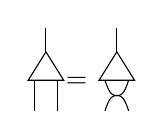
\begin{tikzpicture}[scale=.3]
  \draw (2,1) -- (2,0);
  \draw (2,0) -- (1.25,-1.2) -- (2.75,-1.2) -- cycle;
  \draw (1.5,-1.2) -- (1.5,-2.5);
  \draw (2.5,-1.2) -- (2.5,-2.5);

  \node at (3.3,-1.3) {$=$};

  \draw (5,1) -- (5,0);
  \draw (5,0) -- (4.25,-1.2) -- (5.75,-1.2) -- cycle;
  \draw (4.5,-1.2) .. controls (4.9,-2.5) and (5.1, -1.2) .. (5.5,-2.5);
  \draw (5.5,-1.2)  .. controls (5.1,-2.5) and (4.9, -1.2) .. (4.5,-2.5);
\end{tikzpicture}
% subsubsection diagrammatic_language (end)


Inverse products are extra structure on an inverse category, rather than a property. A concrete
category showing this is given in the following example.

\begin{example}[Showing that inverse product is additional structure.]
  \label{example:invprodisstructure}
\end{example}
Any discrete category (i.e., a category with only the identity arrows) is a trivial inverse
category. To create an inverse product on the category, add a commutative, associative, idempotent
multiplication, with a unit, on the objects.

Label the four objects of $\D$ as $a,b,c$ and $d$. Then, define two different inverse product
tensors by:
\begin{quote}
  \qquad\qquad
  \begin{tabular}{|l||c|c|c|c|}
    \hline
    $\*$&a&b&c&d\\ \hline \hline
    a&a&a&a&a\\ \hline
    b&a&b&\textbf{b}&b\\ \hline
    c&a&\textbf{b}&c&c \\ \hline
    d&a&b&c&d \\ \hline
  \end{tabular}
  \hfil
  \begin{tabular}{|l||c|c|c|c|}
    \hline
    $\*$&a&b&c&d\\ \hline \hline
    a&a&a&a&a\\ \hline
    b&a&b&\textbf{a}&b\\ \hline
    c&a&\textbf{a}&c&c \\ \hline
    d&a&b&c&d \\ \hline
  \end{tabular}
  \qquad \qquad
\end{quote}

The fact that these operations are idempotent(commutative and associative) implies there is a
trivial Frobenius structure.

% subsection inverse_products (end)


\subsection{Discrete inverse categories} % (fold)
\label{sub:discrete_inverse_categories}


An inverse category with inverse products is a \emph{discrete inverse category}. This paper will
now present some properties of discrete inverse categories. These properties will be used later
when describing a functor that lifts the inverse category to a Cartesian restriction category.


\begin{lemma}\label{lem:properties_of_delta_and_tensor_in_a_discrete_inverse_category}
  In a discrete inverse category \X with the tensor $\*$ and $\Delta$ defined as above, where
  $e=\rst{e}$ is a restriction idempotent and $f,g,h$ are arrows in \X, the following are true:
  \begin{enumerate}[{(}i{)}]
    \item{}$e=\Delta (e\* 1) \inv{\Delta}$.\label{le:eisde1}
    \item{}$e\Delta (f \* g) = \Delta (e f \* g) $ (and $= \Delta (f \* e g) $ and
      $ = \Delta (e f \* e g)$.)\label{le:deltaefg}
    \item{}$ (f \* g e) \inv{\Delta} =(f \* g) \inv{\Delta} e $ (and $= (f e\* g) \inv{\Delta}$ and
      $ = (f e\* g e)\inv{\Delta}$.)\label{le:efginvdelta}
    \item{}$\restr{\Delta (f \* g) \inv{\Delta}} =
       \Delta(1\* g \inv{f})\inv{\Delta}$. \label{le:restfg}
    \item{} If $\Delta (h \* g) \inv{\Delta} = \restr{\Delta (h \* g) \inv{\Delta}}$ then
      $(\Delta (h \* g) \inv{\Delta}) h = \Delta (h \* g) \inv{\Delta}$.\label{le:hge}
    \item{}$\Delta (f\*1) = \Delta (g\*1) \implies f = g$.\label{le:dfgisfg}
    \item{}$(f\*1) = (g\*1) \implies f = g$.\label{le:fgisfg}
  \end{enumerate}
\end{lemma}
\begin{proof}
  \prepprooflist
  \begin{enumerate}[{(}i{)}]
    \item[\ref{le:eisde1}]This is shown by proving both sides
      equal $\Delta (e\* 1) \inv{\Delta} \Delta (e\* 1) \inv{\Delta}$.
      \begin{align*}
        \Delta (e\* 1) &\inv{\Delta} \Delta (e\* 1) \inv{\Delta}
        = \Delta (e\* 1) \inv{\Delta} \Delta (1\* e) \inv{\Delta}&\text{cocommutativity}\\
        &=\Delta(e \Delta \* 1) (1\*\inv{\Delta} e) \inv{\Delta} &\text{Frobenius}\\
        &=\Delta(\Delta \* 1) (e\*e\*1) (1\*\inv{\Delta}e)\inv{\Delta}&\Delta\text{natural}\\
        &=\Delta(\Delta \* 1) (e\*e\*1) (1\*e\*e)(1\*\inv{\Delta})\inv{\Delta}&\inv{\Delta}\text{ natural}\\
        &=\Delta (\Delta \*1) (e\* e\* e)(1\* \inv{\Delta})\inv{\Delta}&e\text{ idempotent}\\
        &=\Delta (\Delta \*1) (e\* \inv{\Delta}e)\inv{\Delta}&\inv{\Delta}\text{ natural}\\
        &=\Delta (\Delta \*1) (1\* \inv{\Delta})\inv{\Delta}e&\inv{\Delta}\text{ natural}\\
        &=\Delta \inv{\Delta}\Delta \inv{\Delta}e&\text{Frobenius}\\
        &=e&\Delta\text{ total}.
      \end{align*}
      At the same time,
      \begin{align*}
        \Delta (e\* 1) &\inv{\Delta} \Delta (e\* 1) \inv{\Delta}
        =\Delta(e \Delta \* 1) (e\*\inv{\Delta} 1) \inv{\Delta} &\text{Frobenius}\\
        &=\Delta(\Delta \* 1) (e\*e\*1) (e\*\inv{\Delta})\inv{\Delta}&\Delta\text{natural}\\
        &=\Delta(\Delta \* 1) (e\*e\*1) (e\*1\*1)(1\*\inv{\Delta})\inv{\Delta}&\inv{\Delta}\text{ natural}\\
        &=\Delta (\Delta \*1) (e\* e\* 1)(1\* \inv{\Delta})\inv{\Delta}&e\text{ idempotent}\\
        &=\Delta  (e\Delta\* 1)(1\*\inv{\Delta})\inv{\Delta}&\Delta\text{natural}\\
        &=\Delta (e \* 1) \inv{\Delta}\Delta\inv{\Delta} &\text{Frobenius}\\
        &=\Delta (e \* 1) \inv{\Delta} &\Delta\text{ total}\
      \end{align*}
      which gives $e = \Delta (e \* 1) \inv{\Delta}$.
    \item[\ref{le:deltaefg}]This equality starts by using the previous equality:
      \begin{align*}
        e\Delta &(f \* g) = \Delta (e\* 1) \inv{\Delta} \Delta(f \* g)
          &\text{by part \ref{le:eisde1}}\\
        &=\Delta(e  \* 1) \rst{\inv{\Delta}}(f\*g)&\\
        &=\Delta\rst{\inv{\Delta}}(e \*1)(f\*g)
          & \text{\rtwo as $e\*1$ is a restriction idempotent}\\
        &=\Delta (e f \* g) &\text{ ($f\inv{f} = f$)}.
      \end{align*}
      The second and third equalities follow by cocommutativity, naturality of $\Delta$ and $e$
      being a restriction idempotent.
    \item[\ref{le:efginvdelta}] As in (\vref{le:deltaefg}), details are only given for the
      first equality.
      \begin{align*}
        (f \* g)&\inv{\Delta} e \\
        &= (f \* g) \inv{\Delta}\Delta (1\*e) \inv{\Delta}   &\text{part \ref{le:eisde1}}\\
        &=(f\*g)\rst{\inv{\Delta}}(1\*e) \inv{\Delta}&\\
        &=(f\*g)(1\*e) \rst{\inv{\Delta}}\inv{\Delta}&\rtwo\\
        &=(f\*g e)\inv{\Delta}&\rone
      \end{align*}
      The other equalities follow from co-commutativity, naturality of $\Delta$ and $e$ being
      a restriction idempotent.
    \item[\ref{le:restfg}]Here, we start by using the fact all maps have a partial inverse:
      \begin{align*}
        ~&\restr{\Delta (f \* g) \inv{\Delta} } \\
        &=\Delta (f \* g) \inv{\Delta} \Delta (\inv{f} \* \inv{g}) \inv{\Delta} \\
        &=\Delta (g \* f) \inv{\Delta} \Delta (\inv{g} \* \inv{f}) \inv{\Delta}& \text{co-commutative} \\
        &=\Delta(g\Delta \*f)(\inv{g}\*\inv{\Delta}\inv{f})\inv{\Delta}&\text{Frobenius}\\
        &=\Delta (\Delta\*1)(g \* g \* f)(\inv{g}\*\inv{\Delta}\inv{f})\inv{\Delta}&\Delta \text{ natural}\\
        &=\Delta (\Delta\*1)(g \* g \* f)(\inv{g} \* \inv{f}\* \inv{f})(1\* \inv{\Delta})\inv{\Delta}&\inv{\Delta} \text{ natural}\\
        &=\Delta (\Delta\*1)(\restr{g} \* g \inv{f}\* \restr{f})(1\* \inv{\Delta})\inv{\Delta}&\text{combine maps}\\
        &=\Delta (\Delta\*1)(\restr{g} \* \restr{g}\,g \inv{f}\restr{f}\* \restr{f})(1\* \inv{\Delta})\inv{\Delta}&\text{restriction axioms}\\
        &=\Delta (\restr{g}\Delta\*1)(1\*g\inv{f}\restr{f}\* \restr{f})(1\*\inv{\Delta}) \inv{\Delta}&\Delta \text{ natural}\\
        &=\Delta (\restr{g}\Delta\*1)(1\*g\inv{f}\*1)(1\*\inv{\Delta}\restr{f}) \inv{\Delta}&\inv{\Delta} \text{ natural}\\
        &=\Delta (\Delta\*1)(1 \* \restr{g}g \inv{f}\*1)(1\*\inv{\Delta}\restr{f}) \inv{\Delta}&\text{This lemma(\ref{le:deltaefg})}\\
        &=\Delta (\Delta\*1)(1 \* \restr{g}g \inv{f}\restr{f}\*1)(1\*\inv{\Delta}) \inv{\Delta}&\text{This lemma(\ref{le:efginvdelta})}\\
        &=\Delta (\Delta\*1)(1 \*g \inv{f}\*1)(1\*\inv{\Delta}) \inv{\Delta}&\text{restriction axioms}\\
        &=\Delta c_{A,A}(\Delta\*1)(1 \*g \inv{f}\*1)(1\*\inv{\Delta}) \inv{\Delta}&\text{co-commutative}\\
        &=\Delta (1\*\Delta)c_{A,A\*A}(1 \*g \inv{f}\*1)(1\*\inv{\Delta}) \inv{\Delta}&c_{\*}\text{natural}\\
        &=\Delta (1\*\Delta)(1\*1\*g \inv{f})c_{A,A\*A}(1\*\inv{\Delta}) \inv{\Delta}&c_{\*}\text{natural}\\
        &=\Delta (1\*\Delta)(1\*1\*g \inv{f})(\inv{\Delta}\*1)c_{A,A} \inv{\Delta}&c_{\*}\text{natural}\\
        &=\Delta (1\*\Delta)(1\*1\*g \inv{f})(\inv{\Delta}\*1) \inv{\Delta}&c_{\*}\text{co-commutative}\\
        &=\Delta \inv{\Delta}\Delta (1 \* g \inv{f})\inv{\Delta}&\text{Frobenius}\\
        &=\Delta(1 \* g \inv{f}) \inv{\Delta}&\Delta\text{ total}
      \end{align*}
      Note the pattern in the last few lines of using the co-commutativity of $\Delta$, the
      naturality of the commutativity isomorphism and finishing with the co-commutativity of
      $\inv{\Delta}$. In future proofs, these steps will be combined to a single line and referred to
      as commutativity.
    \item[\ref{le:hge}]Beginning with the assumption,
      \begin{align*}
        (\Delta (h \* g) &\inv{\Delta})h  = \rst{\Delta (h \* g) \inv{\Delta}}h&\\
        &=\Delta(1 \* g \inv{h}) \inv{\Delta}h&\text{This lemma(\ref{le:restfg})}\\
        &=\Delta(1 \* g \inv{h}) \inv{\Delta}\Delta(h\*h)\inv{\Delta}&\Delta\text{ total and natural}\\
        &=\Delta(1 \* g \inv{h}) (\Delta \* 1)(1\*\inv{\Delta})(h\*h)\inv{\Delta}&\text{Frobenius}\\
        &=\Delta(\Delta\*1)(1\*1\*g\inv{h})(1\*\inv{\Delta}) (h\*h)\inv{\Delta}&\Delta \text{ natural}\\
        &=\Delta(\Delta\*1)(1\*1\*g\inv{h})(h\*h\*h)(1\*\inv{\Delta}) \inv{\Delta}&\inv{\Delta}\text{ natural}\\
        &=\Delta(\Delta\*1)(h\*h\*g\inv{h}h)(1\*\inv{\Delta}) \inv{\Delta}&\text{combine terms}\\
        &=\Delta(h\*g\restr{\inv{h}})(\Delta\*1)(1\*\inv{\Delta})\inv{\Delta} &\Delta \text{ natural}\\
        &=\Delta(h\*g\restr{\inv{h}})\inv{\Delta}\Delta\inv{\Delta} &\text{Frobenius}\\
        &=\Delta(h \* g \restr{\inv{h}})\inv{\Delta}&\Delta \text{ total}\\
        &=\Delta(h \* g )\inv{\Delta}\restr{\inv{h}}& \text{part (\ref{le:deltaefg})}\\
        &=\Delta(h\restr{\inv{h}}\*g)\inv{\Delta}&\text{part (\ref{le:deltaefg})}\\
        &=\Delta(h\*g)\inv{\Delta}&\text{property of inverse}.
      \end{align*}

    \item[\ref{le:dfgisfg}]As $\Delta$ is total and natural, we start with:
      \begin{align*}
        f&=\Delta(f\*f)\inv{\Delta}  & \\
        &= \Delta(f\*1)(1\*f)\inv{\Delta} &  \\
        &= \Delta(g\*1)(1\*f)\inv{\Delta} &\text{assumption} \\
        &= \Delta(1\*f)(g\*1)\inv{\Delta} &\text{Identities commute}\\
        &= \Delta(1\*g)(g\*1)\inv{\Delta} &\text{assumption, co-commutative}\\
        &= \Delta(g\*g)\inv{\Delta} \\
        &= g\Delta\inv{\Delta} & \Delta \text{ natural}\\
        &= g&\Delta\text{ total}.
      \end{align*}
    \item[\ref{le:fgisfg}] Immediate from part \vref{le:dfgisfg}.
  \end{enumerate}
\end{proof}

\begin{proposition}
  A discrete inverse category has meets, where $f\cap g =\Delta (f\* g) \inv{\Delta}$.
\end{proposition}
\begin{proof}
  $f\cap g \le f$:
  \begin{align*}
    f\cap g&= \Delta (f\*g) \inv{\Delta}&\text{Definition of }\cap \\
    &= \Delta (f\restr{\inv{f}}\*g) \inv{\Delta} &\text{property of inverse}\\
    &= \Delta (f \* g\restr{\inv{f}}) \inv{\Delta} &\text{by lemma \ref{lem:properties_of_delta_and_tensor_in_a_discrete_inverse_category}(\ref{le:efginvdelta})}\\
    &= \Delta (f \* g\inv{f}f) \inv{\Delta} &\text{definition of inverse}\\
    &= \Delta (1 \* g\inv{f}) \inv{\Delta} f &\inv{\Delta}\text{ natural}\\
    &=\restr{f \cap g} f &\text{by lemma \ref{lem:properties_of_delta_and_tensor_in_a_discrete_inverse_category}(\ref{le:restfg})}\\
  \end{align*}

  $f\cap f = f$:
  \begin{align*}
    f\cap f &= \Delta(f\* f) \inv{\Delta}\\
    &=f \Delta \inv{\Delta} &\Delta\text{ natural}\\
    &= f&\Delta\text{ total}.
  \end{align*}

  $h(f\cap g) = h f \cap hg$:
  \begin{align*}
    h(f\cap g) &= h \Delta(f\* g) \inv{\Delta}& \text{Definition of }\cap\\
    &= \Delta(h \* h) (f \* g) \inv{\Delta} &\Delta\text{ natural}\\
    &= \Delta(h f\* hg) \inv{\Delta} &\text{compose maps}\\
    &= h f \cap hg&\text{Definition of }\cap.
  \end{align*}
\end{proof}
% subsection discrete_inverse_categories (end)


\subsection{The inverse subcategory of a discrete restriction category } % (fold)
\label{sub:the_inverse_subcategory_of_a_discrete_restriction_category}

Given a discrete restriction category, one can pick out the maps which are partial isomorphisms.
Using results from the previous sub-section and from sub-section \vref{sub:graphic_categories},
this section will show that these maps form a restriction subcategory and in fact, form a discrete
inverse category.

\begin{lemma}\label{lem:inv_x_is_a_discrete_inverse_category}
  Given \X is a discrete restriction category, the invertible maps of \X, together with the objects
  of \X form a sub restriction category which is a discrete inverse category, denoted by \Invc{\X}.
\end{lemma}
\begin{proof}
  As shown in Lemma \vref{lem:rcs_partial_monic_section_inverse_properties}, partial isomorphisms
  are closed under composition. The identity maps are in \Invc{\X}. Trivially, restrictions of
  partial isomorphisms are also partial isomorphisms.

  The product on the discrete restriction category \X becomes the tensor product of the restriction
  category \Invc{\X}. Table \vref{tab:structural_maps_for_the_tensor_in_invx} shows how each of the
  elements of the tensor are defined. Note that the last definition makes explicit use of the fact
  we are in a discrete restriction category and hence the $\Delta$ of \X possesses a partial
  inverse.

  \begin{table}[h!]
    \begin{center}
      \begin{tabular}{|ccc|}
        \hline
        \X & \Invc{\X} & Inverse map\\
        \hline\hline
        $\scriptstyle A\times B$ & $\scriptstyle A\* B$ &\\
        \hline
        $\scriptstyle \top$ & $\scriptstyle 1$ &\\
        \hline
        $\scriptstyle \pi_1:\top\times A \to A$ & $\scriptstyle \usl:1\* A \to A$ & $\scriptstyle \<!,1\>$\\
        \hline
        $\scriptstyle \pi_0:A\times\top \to A$ & $\scriptstyle \usr:A\*1 \to A$& $\scriptstyle \<1,!\>$\\
        \hline
        ${\scriptstyle \<\pi_0 \pi_0,\<\pi_0 \pi_1,\pi_1\>\>:(A\times B)\times C \to A\times(B\times C)}$
          & $\scriptstyle a_{\*}:(A\*B)\*C \to A\*(B\*C)$
          & $\scriptstyle \<\<\pi_0, \pi_1 \pi_0\>,\pi_1 \pi_1\>$\\
        \hline
        $\scriptstyle \< \pi_1,\pi_0\>:A\times B \to B\times A$ & $\scriptstyle c_{\*}:A\*B \to B \* A$ & $\scriptstyle \< \pi_1,\pi_0\>$\\
        \hline
        $\scriptstyle \Delta_{\X}:A\to A\times A$ & $\scriptstyle \Delta:A \to A\* A$ & $\scriptstyle  \inv{\Delta_{\X}} $\\
        \hline
      \end{tabular}

    \end{center}
    \caption{Structural maps for the tensor in \Invc{\X}}
    \label{tab:structural_maps_for_the_tensor_in_invx}
  \end{table}

  The monoid coherence diagrams and $\Delta$ being total follow directly from the characteristics
  of the product in \X. It remains to show co-commutativity, co-associativity and the Frobenius
  condition.

  Co-commutativity requires $\Delta c_{\*} = c_{\*}$. From the definitions, this means we need
  \[\Delta_{\X} \< \pi_1,\pi_0\> = \Delta_{\X}.\] Once again, this follows immediately from the
  definition of restriction product.

  Co-associativity requires $\Delta (1 \* \Delta) = \Delta (\Delta \* 1) a_{\*}$. Expressing this
  in \X, we require
  \[
    \Delta_{\X} (1 \times \Delta_{\X}) =
      \Delta_{\X}(\Delta_{\X} \times 1) (\<\pi_0 \pi_0,\<\pi_0 \pi_1,\pi_1\>\>).
  \]
  Again each is equal based on the properties of the restriction product.

  The Frobenius requirement is two-fold:
  \begin{align}
    \inv{\Delta} \Delta &= (\Delta \*1) a_{\*}(1\*\inv{\Delta}) \label{eq:frobenius_righths_need_in_invx}\\
    \inv{\Delta} \Delta &= (1 \* \Delta) \inv{a_{\*}}(\inv{\Delta}\* 1), \label{eq:frobenius_lefths_need_in_invx}
  \end{align}
  but in \X, this becomes:
  \begin{align}
    \inv{\Delta_{\X}} \Delta_{\X}
      &= (\Delta_{\X} \times 1) \<\pi_0 \pi_0,\<\pi_0 \pi_1,\pi_1\>\>(1\times\inv{\Delta_{\X}})
      \label{eq:frobenius_righths_expressed_in_x}\\
    \inv{\Delta_{\X}}\Delta_{\X}
      &= (1 \times \Delta_{\X}) \<\<\pi_0, \pi_1 \pi_0\>,\pi_1 \pi_1\>(\inv{\Delta_{\X}}\times 1).
      \label{eq:frobenius_lefths_expressed_in_x}
  \end{align}
  We will detail the proof of equation \vref{eq:frobenius_righths_expressed_in_x}. Equation
  \vref{eq:frobenius_lefths_expressed_in_x} is proved similarly.

  To show the equation, note first that $\Delta(1 \times !)$ (and $\Delta(!\times 1)$) is the
  identity and secondly that maps to a product of objects may be split into a product map --- e.g.
  if $f:A \to B \times B$, then $f = \<f(1\times !), f(!\times 1)\>$.

  Using this we see that the left hand side of equation \vref{eq:frobenius_righths_expressed_in_x}
  computes as follows:
  \begin{align*}
    \inv{\Delta_{\X}} \Delta_{\X}
      & = \<\inv{\Delta_{\X}} \Delta_{\X}(1\times !), \inv{\Delta_{\X}} \Delta_{\X} (! \times 1)\>\\
    &= \<\inv{\Delta_{\X}}, \inv{\Delta_{\X}} \>
  \end{align*}
  Similarly, removing the associativity maps, the right hand side of the same equation becomes:
  \begin{align*}
    (\Delta_{\X} \times 1) (1\times\inv{\Delta_{\X}}) &
      = \<(\Delta_{\X} \times 1) (1\times\inv{\Delta_{\X}}) (1\times !),
      (\Delta_{\X} \times 1) (1\times\inv{\Delta_{\X}}) (! \times 1 )\> \\
    &= \<(\Delta_{\X} \times 1) (1\times\inv{\Delta_{\X}}) (1\times ! ), \inv{\Delta_{\X}}\> \\
    &= \<(\Delta_{\X} \times 1) (1\times\inv{\Delta_{\X}}) (1 \times \Delta_{\X})(1\times !\times !), \inv{\Delta_{\X}}\> \\
    &= \<(\Delta_{\X} \times 1) (1\times\rst{\inv{\Delta_{\X}}}) (1\times !\times !), \inv{\Delta_{\X}}\> \\
    &= \<(\Delta_{\X} \times 1) \rst{1\times\inv{\Delta_{\X}}} (1\times !\times !), \inv{\Delta_{\X}}\> \\
    &= \<\rst{(\Delta_{\X} \times 1) (1\times\inv{\Delta_{\X}})}
      (\Delta_{\X} \times 1)(1\times !\times !), \inv{\Delta_{\X}}\> \\ %rfour
    &= \<\rst{(\Delta_{\X} \times 1) (1\times\inv{\Delta_{\X}})} (1\times !), \inv{\Delta_{\X}}\> \\
      &= \<\rst{(\Delta_{\X} \times 1) (1\times\inv{\Delta_{\X}})(! \times 1)} (1\times !),
      \inv{\Delta_{\X}}\> \\ % add total to right of rst
    &= \<\rst{\inv{\Delta_{\X}}} (1\times !), \inv{\Delta_{\X}}\> \\
    &= \<\inv{\Delta_{\X}}\Delta_{\X}(1\times !), \inv{\Delta_{\X}}\> \\
    &= \<\inv{\Delta_{\X}}, \inv{\Delta_{\X}}\>
  \end{align*}
  and therefore we see that the first equation for the Frobenius condition is satisfied. Thus,
  $Inv(\X)$ is a discrete inverse category.
\end{proof}
% subsection the_inverse_subcategory_of_a_graphic_cartesian_restriction_category (end)

% section inverse_products (end)

\section{Completing a discrete inverse category} % (fold)
\label{sec:completing_a_discrete_inverse_category}

The purpose of this section is to prove that the category of discrete inverse categories is
equivalent to the the category of discrete restriction categories. In order to prove this, we show
how to construct a discrete restriction category, \Xt, from a discrete inverse category, \X.


\subsection{The restriction category \hypXt} % (fold)
\label{sub:the_restriction_category_hypxt}

\begin{definition}\label{def:xt}

  When \X is an inverse category, define \Xt\ as:
  \category{objects as in \X}
  {
    equivalence classes of maps (the equivalence class is defined below in Definition
    \vref{defn:xequivalence}) with the following structure in \X: %
    \[
      \infer{A\xrightarrow{f} B\*C \text{ in }\X}{A \xrightarrow{\ (f,C)\ } B \text{ in } \Xt}
      \]
  }
  {% identity
    by
    \[
      \infer{A\xrightarrow{\inv{u_{\*}^r}}A\* 1}
            {A \xrightarrow{(\inv{u_{\*}^r}, 1)} A}
    \]
  }
  {% composition
    given by
    \[
      \infer{
        \infer{A\xrightarrow{(f (g\*1) a_{\*},C' \* B')} C}
              {A\xrightarrow{f (g\*1) a_{\*}} C \* (C' \* B')}
            }
            {A \xrightarrow{\ (f,B')\ } B \xrightarrow{\ (g,C')\ } C}
    \]
  }

\end{definition}

When considering an \Xt\ map $(f,C):A\to B$ in \X, we occasionally use the notation $f:A\to
\xtdmn{B}{C}$ ($\equiv f:A\to B\* C$).

\subsubsection{Equivalence classes of maps in \hypX} % (fold)
\label{ssub:equivalence_classes_of_maps_in_hypx}


\begin{definition}\label{defn:xequivalence}
  In a discrete inverse category \X as defined above, the map $f$ is equivalent to $f'$ in \X when
  $\restr{f} = \restr{f'}$ in \X and the below diagram commutes for some map $h$:
  \[
    \xymatrix @C=40pt @R=15pt{
      & & B \* C \ar@{.>}[dr]^{(\Delta\* 1) \, a_{\*}}\\
      && & B \* (B\* C) \ar@{.>}[dd]^{1\* h} \\
      A \ar[uurr]^f \ar[ddrr]_{f'}&&&\\
      && & B \* (B \* C') \ar@{.>}[dl]^(.4){\ \inv{a_{\*}}\,(\inv{\Delta}\* 1)}\\
      && B\* C'
    }
  \]
\end{definition}

\begin{notation}
  When $f$ is equivalent to $g$ via the mediating map $h$, this is written as
  \[
    f\xequiv{h}g.
  \]
\end{notation}


\begin{lemma}\label{lem:mediating_map_equivalence_is_symmetric_reflexive_and_transitive}
  Definition \vref{defn:xequivalence} gives a symmetric, reflexive equivalence class of maps in \X.
\end{lemma}
\begin{proof}
  \prepprooflist
  \begin{description}
    \itembf{Reflexivity: } Choose $h$ as the identity map.
    \itembf{Symmetry: } Suppose $f\xequiv{h}g$. Then, $\restr{f} = \restr{g}$ and $f k = g$ where
      \[
        k = (\Delta\* 1) \, a_{\*}\, (1\*h)\, \inv{a_{\*}}\,(\inv{\Delta}\* 1).
      \] Applying $\inv{k}$,
      which is
      \[
        (\Delta\* 1) \, a_{\*}\, (1\*\inv{h})\, \inv{a_{\*}}\,(\inv{\Delta}\* 1),
      \]
      we have
      \[
        g \inv{k} = f k \inv{k} = f \restr{k} = \restr{f k} f
        = \restr{g} f = \restr{f} f = f.
      \]

      Thus, $g\xequiv{\inv{h}} f$.

    \itembf{Transitivity: } Suppose $f\xequiv{h} f'$ and $f' \xequiv{k} f''$. Then, consider the
      compositions of the mediating portions of the equivalences:
      \[
        \ell = ((\Delta \* 1)  a_{\*}  (1 \* h ) \inv{a_{\*}} (\inv{\Delta}\* 1))
          ( (\Delta \* 1) a_{\*}  (1 \* k) \inv{a_{\*}} (\inv{\Delta}\* 1)).
      \]
      By pasting the diagrams which give the above equivalences, we see that $f \ell = f''$.
      However, it is not in the form of a mediating map as presented.

      The claim is that $\ell$ is the actual mediating map for $f$ and $f''$. That is, that we have
      $f(\Delta \* 1)a_{\*}(1 \* \ell)\inv{a_{\*}}(\inv{\Delta}\*1) = f''$. In the interest of some
      brevity, this is shown below with the associativity maps elided from the equations.

      We need to show that $(\Delta \* 1)(1 \* \ell)(\inv{\Delta}\*1) = \ell$.
      \begin{align*}
        (\Delta \* 1)&(1 \* \ell)(\inv{\Delta}\*1) \\
        &=
          (\Delta \* 1)(1\*\Delta \* 1)  (1\*1 \* h ) (1\*\inv{\Delta}\* 1))\\
          &\qquad\qquad\qquad
            (1\*\Delta \* 1) (1\* 1 \* k) (1\*\inv{\Delta}\* 1)(\inv{\Delta}\* 1)\\
        &=
          (\Delta \* 1)(\Delta \* 1\*1)  (1\*1 \* h ) (1\*\inv{\Delta}\* 1))\\
          & \qquad\qquad\qquad
            (1\*\Delta \* 1) (1\* 1 \* k) (\inv{\Delta}\*1\* 1)(\inv{\Delta}\* 1)
              &\text{co-associativity}\\
        &=
          (\Delta \* 1)  (1 \* h ) (\Delta \* 1\*1)(1\*\inv{\Delta}\* 1)) \\
          &\qquad\qquad\qquad
            (1\*\Delta \* 1)  (\inv{\Delta}\*1\* 1)(1 \* k)(\inv{\Delta}\* 1)&\text{Naturality}\\
        &=
          (\Delta \* 1)  (1 \* h ) (\inv{\Delta} \*1)(\Delta\* 1)) \\
          &\qquad\qquad\qquad
            (\inv{\Delta} \* 1)  (\Delta \* 1)(1 \* k)(\inv{\Delta}\* 1)&\text{Frobenius}\\
        &=
          (\Delta \* 1)  (1 \* h ) (\inv{\Delta} \*1)
          (\Delta \* 1)(1 \* k)(\inv{\Delta}\* 1)&\Delta\text{ Total}\\
        &= \ell
      \end{align*}
  \end{description}
  and therefore $f\xequiv{\ell}f''$.
\end{proof}

\begin{corollary}\label{cor:equivalence_simplified_diagram}
  If $\restr{f} = \restr{g}$ in \X, a discrete inverse category, and the diagram
  \[
    \xymatrix @C=40pt @R=15pt{
      & & B \* C \ar@{.>}[dd]^{1\*h}\\
      A \ar[urr]^f \ar[drr]_{g}\\
      && B\* C'
    }
  \]
  commutes for some $h$, then there is a $h'$ such that $f\xequiv{h'}g$.
\end{corollary}
\begin{proof}
  Consider
  \begin{align*}
    (\Delta \*1)\,a_{\*}\,(1\*(1\*h))\,&\inv{a_{\*}}(\inv{\Delta}\*1)\\
    & = (\Delta \*1)\,((1\*1)\*h)\,a_{\*}\inv{a_{\*}}(\inv{\Delta}\*1) & \text{Naturality}\\
    &=(\Delta \*1)\,((1\*1)\*h)\,(\inv{\Delta}\*1) & \text{Isomorphism Inverse}\\
    &=(\Delta (1\*1) \inv{\Delta})\* h & \text{Naturality of }\*\\
    &=(1\* h) & \Delta  \inv{\Delta}=1\\
  \end{align*}
  and therefore we can set $h' = 1 \* h$.
\end{proof}



\begin{lemma}\label{lem:xt_is_a_category}
  \Xt\ as defined above is a category.
\end{lemma}
\begin{proof}
  The maps are well defined, as shown in lemma
  \vref{lem:mediating_map_equivalence_is_symmetric_reflexive_and_transitive}. The existence of the
  identity map is due to the tensor $\*$ being defined on \X, an inverse category, hence
  $\inv{\usr}$ is defined.

  It remains to show the composition is associative and that $(\inv{\usr}, 1)$ acts as an identity
  in \Xt.

  \textbf{Associativity:}
  Consider
  \[
    A\xrightarrow{(f,B')}B\xrightarrow{(g,C')} C \xrightarrow{(h,D')}D.
  \]

  To show the associativity of this in \Xt, we need to show in \X that
  \[
    \restr{(f(g\*1)a_{\*}) (h\*1)a_{\*}} = \restr{f (((g(h\*1)a_{\*})\*1) a_{\*})}
  \]
  and that there exists a mediating map between the two of them.

  To see that the restrictions are equal, first note that by the functorality of $\*$, for any two
  maps $u$ and $v$, we have $u v \* 1 = (u\*1) (v\*1)$. Second, the naturality of $a_{\*}$ gives us
  that $a_{\*} (h \* 1) = ((h\*1)\*1) a_{\*}$. Thus,
  \begin{align*}
    \restr{f(g\*1)a_{\*} (h\*1)a_{\*}}
      & = \restr{f(g\*1)a_{\*} (h\*1)\restr{a_{\*}}}
    & \text{Lemma \ref{lem:restrictionvarious}} \\
    & = \restr{f(g\*1)a_{\*} (h\*1)} & \restr{a_{\*}}=1 \\
    & = \restr{f(g\*1) ((h\*1)\*1) a_{\*} } & a_{\*}\text{ natural} \\
    & = \restr{f(g\*1) ((h\*1)\*1) }
      & a_{\*}   \text{ iso, Lemma \ref{lem:restrictionvarious}}\\
    & = \restr{f(g\*1) ((h\*1)\*1) (a_{\*}\*1)}
      & a_{\*}\*1 \text{ iso, Lemma \ref{lem:restrictionvarious}}\\
    & = \restr{f((g (h\*1)a )\*1)} & \text{ see above}\\
    & = \restr{f((g (h\*1)a )\*1)a_{\*}} & a_{\*}   \text{ iso}
  \end{align*}

  For the mediating map, see the diagram below, where calculation is in \X. The path starting at
  the top left at $A$ and going right to \xtdmn{D}{D' \* (C' \* B')} is grouping parentheses to the
  left, while starting in the same place but going down to $\xtdmn{(\xtdmn{D}{D' \* C'})}{B'}$ and
  then right to $ \xtdmn{D}{(D' \* C') \* B'}$ is grouping parentheses to the right. The
  commutativity of the diagram is shown by the commutativity of the internal portions, which all
  follow from the standard coherence diagrams for the tensor and naturality of association.

  \[
    \xymatrix @C=30pt @R=45pt{
      A \ar[d]_f \ar[r]^(.4){f (g\*1) a_{\*}} \ar[dr]^(.4){f(g\*1)} &
        \xtdmn{C}{C' \* B'} \ar[r]^{h\*1}
        & \xtdmn{(\xtdmn{D}{D'})}{C' \* B'} \ar[r]^{a_{\*}}
        & \xtdmn{D}{D' \* (C' \* B')}
        \ar@{.>}[dd]^{1\*\inv{a_{\*}}}\\
      \xtdmn{B}{B'} \ar[d]_{(g (h\*1) a_{\*})\*1} \ar[r]_{g\*1}
        &\xtdmn{(\xtdmn{C}{C'})}{B'} \ar[u]_{a_{\*}} \ar[r]_(.4){(h\*1)\*1}
        & \xtdmn{(\xtdmn{(\xtdmn{D}{D'})}{C'})}{B'}
        \ar[u]_{a_\*} \ar[dll]_{a_{\*}\*1}
      \\
      \xtdmn{(\xtdmn{D}{D' \* C'})}{B'}  \ar[rrr]_{a_{\*}}
        &&& \xtdmn{D}{(D' \* C') \* B'} %\ar @/^14pt/ [uu]^{1\*a_{\*}}
    }
  \]
  From this, we can conclude
  \[
    (f(g\*1)a_{\*}) (h\*1)a_{\*} \xequiv{1\*\inv{a_{\*}}} f (((g(h\*1)a_{\*})\*1) a_{\*})
  \]
  which gives us that composition in \Xt is associative.

  \textbf{Identity:} This requires:
  \[
    (f,C) (\inv{\usr}, 1) = (f,C) = (\inv{\usr}, 1) (f,C)
  \]
  for all maps $A\xrightarrow{(f,C)}B$ in \Xt.

  First, we see $\restr{f (\inv{\usr}\*1) a_{\*}} = \restr{f}$ by Lemma
  \vref{lem:restrictionvarious}. Then, calculating in \X, we have a mediating map of
  $1 \* \usl$ as shown below.
  \[
    \xymatrix @C=50pt @R=45pt{
      A \ar[r]^f \ar[ddrrr]_f&
        B \* C \ar[r]^(.4){\inv{\usr}\*1}
        \ar@/_20pt/[rr]_{1 \* \inv{\usl}}
        \ar@{=}[ddrr]
        & (B \* 1) \* C \ar[r]^{a_{\*}}
        & B \* (1 \* C) \ar@{.>}[dd]^{1 \* \usl} \\
      \\
      &&& B \* C
    }
  \]

  Next, $\restr{\inv{\usr} (f \*1)  a_{\*}} = \restr{f}$ by the naturality of $\inv{\usr}$ and
  Lemma \vref{lem:restrictionvarious}. The diagram below
  \[
    \xymatrix @C=50pt @R=45pt{
      A \ar@{=}[dd] \ar[r]^{\inv{\usr}} \ar[dr]_{f}
        &      A \* 1 \ar[r]^{f \* 1}
        & (B \* C) \* 1 \ar[r]^{a_{\*}}
        & B \* (C \* 1)\ar@{.>}[dd]^{1 \* \usr} \\
      &B\*C \ar[ur]^{\inv{\usr}} \ar[urr]_{1\*\inv{\usr}} \ar@{=}[drr]\\
      A \ar[rrr]^f &&& B \* C
    }
  \]
  shows our mediating map is $1 \* \usr$.
\end{proof}
% subsubsection equivalence_classes_of_maps_in_hypx (end)

\subsubsection{Defining the restriction on \hypXt} % (fold)
\label{ssub:defining_the_restriction_on_hypxt}



Define the restriction in \Xt\ as follows:
\[
  \infer{A\xrightarrow{\restr{f}  \inv{u_{\*}^r}} A\*1 \text{ in }\X}
        {\infer{A\xrightarrow{\restr{(f,C)}}A}
               {A\xrightarrow{(f,C)}B}
        }
\]

\begin{lemma}\label{lem:xt_is_a_restriction_category}
  The category \Xt with restriction defined as above is a restriction category.
\end{lemma}
\begin{proof}

  Given the above definition, the four restriction axioms must now be checked. (Diagrams are in \X).
  \begin{description}
    \item[\rone] ($\restr{f} f = f$) Calculating the restriction of the left hand side in
      \X, we have:
      \begin{align*}
        \restr{\rst{f}\inv{\usr} (f\*1) a_{\*}} & = \restr{\rst{f}\inv{\usr} (f\*1)}
          & a_{\*}   \text{ iso, Lemma \ref{lem:restrictionvarious}}\\
        & = \restr{\rst{f}f \inv{\usr}}  & \inv{\usr} \text{ natural}\\
        & = \restr{f \inv{\usr}}  & \text{ \rone in }\X\\
        & = \restr{f } & \inv{\usr}   \text{ iso, Lemma \ref{lem:restrictionvarious}}.
      \end{align*}

      Then, the following diagram
      \[
        \xymatrix @C=40pt @R=25pt{
          A \ar[r]^{\restr{f} \inv{\usr}}
          \ar @/_25pt/[ddrrr]_f  \ar[drr]^{\restr{f}f}
          &A \* 1 \ar[r]^{f\* 1}
          &(A \* B) \* 1 \ar[r]^{a_{\*}} \ar[ddr]^{\usr}
          &A \* (B \* 1) \ar@{.>}[dd]^{1 \* {\usr}}\\
          &&A\*B \ar[u]^{\inv{\usr}} \ar@{=} [dr]\\
          && &A \* B
        }
      \]
      shows $\rst{f}\inv{\usr} (f\*1) a_{\*} \xequiv{1 \* {\usr}} f$ in \X and therefore $\rst{f}f
      = f$ in \Xt.


    \item[\rtwo] ($\restr{g} \restr{f} = \restr{f} \restr{g}$) The restriction of the left hand
      side equals the restriction of the right hand side as seen below:
      \begin{align*}
        \restr{\rst{f}\inv{\usr} ((\restr{g}\inv\usr)\*1)) a_{\*}} & = \restr{\rst{f}(\restr{g}\inv\usr)\inv{\usr} a_{\*}} & \inv{\usr}   \text{ natural}\\
        & = \restr{\rst{g}\restr{f}\inv\usr\inv{\usr} a_{\*}} &  \text{\rtwo in }\X\\
        & = \restr{\rst{g}\inv{\usr}((\restr{f}\inv\usr)\*1) a_{\*}} & \inv{\usr}   \text{natural}.
      \end{align*}

      %\note{!!!!! Above calc works without being under restr, therefore have we not just shown
      %that $\restr{g}  \restr{f} = \restr{f}  \restr{g}$ ????
      %Note that the mediating map is $id$!!!!!!!!!}

      The below diagram commutes by the naturality of $\usr$ and the tensor coherence,
      \[
        \xymatrix @C=48pt @R=55pt{
          A \ar[r]^{\restr{g} \inv{\usr}}
            \ar[dr]_{\restr{f}\restr{g}}^{\restr{g}\restr{f}}
            \ar[d]_{\restr{f}\inv{\usr}}
            &A\*1 \ar[r]^(.4){(\rst{f}\inv{\usr})\*1}
            & (A \*1) \* 1
            \ar[r]^{a_{\*}}  \ar[dl]_{\usr \usr}
            & A \* (1\*1) \ar@{.>}[dd]_{1\*id}\\ %\ar @/^25pt/ @{=}[dd]
          A\*1 \ar[d]_{(\rst{g}\inv{\usr})\*1}
            &A \ar@/_25pt/[ur]_{\inv{\usr}\inv{\usr}} \\
             %\ar@/^25pt/[dl]^(.3){\inv{\usr}\inv{\usr}}\\
          (A\*1)\*1 \ar[rrr]_{a_\*} \ar[ur]^{\usr \usr}
            &&& A \* (1\*1)
        }
      \]
      which allows us to conclude $\rst{f} \rst{g} = \rst{g} \rst{f}$ in \Xt.



    \item[\textbf{R.3}] ($\restr{\restr{f} g} = \restr{f} \restr{g}$ ). As above, the first step is
      to show that the restrictions of each side are the same. Computing the restriction of the left
      hand side in \X:
      \begin{align*}
        \rst{\restr{(\restr{f} \inv{\usr}) (g\* 1) a_{\*}} \inv{\usr}}
        & = \rst{\restr{(\restr{f} \inv{\usr}) (g\* 1) a_{\*}}} & \inv{\usr}
          \text{ iso, Lemma \ref{lem:restrictionvarious}}\\
        & = \restr{(\restr{f} \inv{\usr}) (g\* 1) a_{\*}} &
          \text{Lemma \ref{lem:restrictionvarious}}\\
        & = \restr{\restr{f} g \inv{\usr} a_{\*}} & \inv{\usr} \text{ natural}\\
        & = \restr{\restr{f} g } & \inv{\usr}, a_{\*}
          \text{ iso, Lemma \ref{lem:restrictionvarious}}\\
        & = \restr{f} \rst{g} & \text{\rthree in }\X.
      \end{align*}
      The restriction of the right hand side computes in \X as:
      \begin{align*}
        \rst{(\restr{f} \inv{\usr}) (\rst{g} \inv{\usr}\* 1) a_{\*}}
        & = \rst{(\restr{f} \inv{\usr}) (\rst{g} \inv{\usr}\* 1) } &  a_{\*}
          \text{ iso, Lemma \ref{lem:restrictionvarious}}\\
        & = \rst{\restr{f}  \rst{g} \inv{\usr}\inv{\usr} } &  \inv{\usr} \text{ natural}\\
        & = \rst{\restr{f}  \rst{g} } &\inv{\usr}\inv{\usr}
          \text{ iso, Lemma \ref{lem:restrictionvarious}}\\
        & = \restr{f} \rst{g} & \text{Lemma \ref{lem:restrictionvarious}}.
      \end{align*}

      Additionally, we see $\rst{\rst{f} g}$ in \Xt is expressed in \X as:
      \begin{align*}
        \restr{(\restr{f} \inv{\usr}) (g\* 1) a_{\*}} \inv{\usr}
        & = \rst{f} \inv{\usr} \rst{g\* 1} & \text{\rthree, \rfour, }a_{\*} \text{ iso} \\
        & = \rst{f} \rst{g} \inv{\usr} & \*
          \text{a restriction bi-functor, }\inv{\usr}\text{ natural.}
      \end{align*}

      The following diagram in \X follows the above right hand side with the top curved arrow and
      the left hand side with the bottom curved arrow. Note that we are using that
      $\restr{(\restr{f} \inv{\usr}) (g\* 1) a_{\*}} = \restr{f}\rst{g}$ as shown above.
      \[
        \xymatrix @C=33pt @R=20pt{
          A \ar@/^45pt/[rrrrr]^{\restr{f} \inv{\usr}(\restr{g} \inv{\usr} \* 1)a_{\*}}
            \ar@/_65pt/[dddddrrrrr]_{\restr{f}\, \restr{g}\inv{\usr}}
            \ar[r]^(.7){\restr{f}}
            \ar[dr]_(.7){\restr{f}}
            &A \ar[r]^{\inv{\usr}}
            \ar@{=}[d]
            &A \* 1 \ar[r]^{\restr{g}\*1}
            \ar[dd]_{\usr}
            &A \* 1 \ar[r]^(.41){\inv{\usr}\* 1}
            \ar[ddd]_{\usr}
            &(A \* 1) \* 1 \ar[r]^{a_{\*}}
            \ar[dddd]_{\usr}
            & A \* (1\*1) \ar@{.>}[ddddd]^{1\*\usr}\\
          &A\ar@{=}[dr]\\
          &&A \ar[dr]_{\restr{g}}\\
          &&&A \ar[dr]_{\inv\usr}\\
          &&&&A\*1 \ar@{=}[dr]\\
          &&&&&A\*1
        }
      \]
      Hence, in \X, $\restr{(\restr{f} \inv{\usr}) (g\* 1) a_{\*}} \inv{\usr} \xequiv{1\*\usr}
      (\restr{f} \inv{\usr}) (\rst{g} \inv{\usr}\* 1) a_{\*}$ and therefore $\restr{\restr{f} g} =
      \restr{f} \restr{g}$ in \Xt.



    \item[\textbf{R.4}] $f \restr{g} = \restr{f g} f$ The restriction of the left hand side is:
      \begin{align*}
        \rst{f (\restr{g} \inv{\usr}\* 1) a_{\*}}
          & = \rst{f (\restr{g} \inv{\usr}\* 1)} & a_{\*}
          \text{ iso, Lemma \ref{lem:restrictionvarious}} \\
        & = \rst{f \rst{g} \inv{\usr}} \* \rst{f} & \* \text{ restriction functor}\\
        & = \rst{f \rst{g}} \* \rst{f} & \inv{\usr}
          \text{ iso, Lemma \ref{lem:restrictionvarious}} \\
        & = \rst{f (\rst{g} \* 1)}
      \end{align*}
      and the restriction of the right hand side is:
      \begin{align*}
        \rst{\rst{f (g \* 1)} \inv{\usr} (f\* 1) a_{\*}}
          & = \rst{\rst{f (g \* 1)} \inv{\usr} (f\* 1) } & a_{\*}
          \text{ iso, Lemma \ref{lem:restrictionvarious}}\\
        & = \rst{\rst{f (g \* 1)} f \inv{\usr}  } & \inv{\usr} \text{ natural}\\
        & = \rst{f \rst{(g \* 1)}  \inv{\usr}  } & \text{ \rfour for }\X\\
        & = \rst{f (\rst{g} \* 1)  \inv{\usr}  } & \* \text{ is a restriction functor}\\
        & = \rst{f (\rst{g} \* 1)    } & \inv{\usr}
          \text{ iso, Lemma \ref{lem:restrictionvarious}}
      \end{align*}

      Computing the right hand side in \X,
      \begin{align*}
        \rst{f(g\* 1)a_{\*}} \inv{\usr} (f\* 1) a_{\*}
          & = \rst{f(g\* 1)} f \inv{\usr} a_{\*} & a_{\*} \text{ iso, } \inv{\usr}\text{ natural.}\\
        & = f (\rst{g} \* 1) \inv{\usr} a_{\*} & \rthree, \* \text{ a restriction functor.}
      \end{align*}
      \[
        \xymatrix @C=40pt @R=35pt{
          A \ar[r]^f \ar[dr]_{f}
            & B\* C \ar[rr]^{\restr{g} \inv{\usr}\* 1}
            &
            & (B\* 1) \* C \ar[r]^{a_{\*}}
            & B \* (1 \* C)\ar@{.>}[d]^{1\*c_{\*}}\\
          & B\*C \ar[r]_{\rst{g}\*1}
            & B \* C \ar[r]_{\inv{\usr}}
            & (B \* C) \* 1 \ar[r]_{a_{\*}}
            & B \* (C\*1)
        }
      \]
  \end{description}

  and hence, \Xt\ is a restriction category.
\end{proof}
% subsubsection defining_the_restriction_on_hypxt (end)
% subsection the_restriction_category_hypxt (end)
\subsection{The category \hypXt is a discrete restriction category} % (fold)
\label{sub:the_category_hypxt_is_cartesian}



\begin{lemma}\label{lem:tensor_unit_of_x_is_terminal_object_of_xt}
  The unit of the inverse product in \X is the terminal object in \Xt.
\end{lemma}
\begin{proof}
  The unique map to the terminal object for any object $A$ in \Xt is the equivalence class of maps
  represented by $(\inv{\usl},A)$. For this to be a terminal object, the diagram
  \[
    \xymatrix @C=40pt @R=25pt{
      X \ar[r]^{\restr{(f,C)}} \ar[d]^{(f,C)} & X \ar[r]^{!_X}  &\top  \\
      Y \ar[urr]_{!_Y}
    }
  \]
  must commute for all choices of $f$. Translating this to \X, this is the same as requiring
  \[
    \xymatrix @C=40pt @R=25pt{
      X \ar[r]^{\restr{f}} \ar[d]^{f} & X \ar[r]^{\inv{\usr} }
      & X\*1 \ar[r]^{\inv{\usl}}  &1\*X\*1 \ar@{.>}[dl]_{1\*(\usr f)}  \\
      Y \*C\ar[rr]_{\inv{\usl}} & & 1 \*Y \* C
    }
  \]
  commute, which is true by \rone and from the coherence diagrams for the inverse product tensor.
\end{proof}

Next,we show that the category \Xt\ has restriction products, given by the the action of \wtc on
the $\*$ tensor in \X.

First, define total maps $\pi_0$, $\pi_1$ in \Xt by:
\begin{align}
  \pi_0:\qquad & A \* B \xrightarrow{(1,B)} A \label{eq:defn:pia}\\
  \pi_1:\qquad & A \* B \xrightarrow{(c_{\*},A)} B \label{eq:defn:pib}
\end{align}
Given the maps $ Z \xrightarrow{(f,C)} A$ and $Z \xrightarrow{(g,C')} B$, define $\<(f,C),(g,C')\>$
as
\begin{equation}
  Z\xrightarrow{(\Delta  ( f \* g )  (1\* c_{\*} \* 1), C\* C')} A \* B\label{eq:defn:fg}
\end{equation}
where associativity is assumed as needed. Note that with the associativity maps, this is actually:
\begin{equation}
  Z\xrightarrow{(\Delta  ( f \* g )  a_{\*} (1\*\inv{a_{\*}})
  (1\* (c_{\*} \* 1)) (1\*a_{\*}) \inv{a_{\*}}, C\* C')} A \* B\label{eq:defn:fg2}
\end{equation}
\begin{lemma}\label{lem:tensor_on_x_is_the_restriction_product_on_xt}
  On \Xt, $\*$ is a restriction product with projections $\pi_0, \pi_1$ with the product of maps
  $f, g$ being $\<f,g\>$.
\end{lemma}
\begin{proof}
  From the definition above, as $1$ and $c_{\*}$ are isomorphisms, the maps $\pi_0, \pi_1$ are
  total.

  In order to show that $\rst{\<f,g\>} = \rst{f}\,\rst{g}$, first reduce the left hand side:
  \begin{align*}
    \rst{\<f,g\>}
      &=\rst{\Delta(f\*g)(1\*c_{\*}\*1)}\inv{\usr}&\text{in }\X, \text{ definition of restriction}\\
    &=\rst{\Delta(f\*g)}\inv{\usr} &c_{\*}\text{ is iso}\\
    &=\rst{\Delta\rst{(f\*g)}}\inv{\usr} &\text{from Lemma \ref{lem:restrictionvarious}}\\
    &=\rst{\Delta(\rst{f}\*\rst{g})}\inv{\usr} &\*\text{ is a restriction functor}\\
    &=\rst{\rst{f}\,\rst{g}\,\Delta(1\*1)}\inv{\usr} &\text{Lemma  \ref{lem:properties_of_delta_and_tensor_in_a_discrete_inverse_category}(\ref{le:deltaefg}) twice}\\
    &=\rst{\rst{f}\,\rst{g}}\inv{\usr} &\text{Lemma  \ref{lem:restrictionvarious}}\\
    &=\rst{f}\,\rst{g}\inv{\usr}  &\text{Lemma  \ref{lem:restrictionvarious}.}\\
  \end{align*}

  Then, the right hand side reduces as:
  \begin{align*}
    \rst{f} \rst{g}
    &= \rst{f}\inv{\usr}(\rst{g}\inv{\usr} \* 1) a_{\*} & \text{in \X by definitions}\\
    &= \rst{f} \rst{g}\inv{\usr}\inv{\usr} a_{\*} &  \inv{\usr}\text{ natural.}
  \end{align*}
  The restriction of the left hand side and the right hand side, in \X, is $\rst{\rst{f} \rst{g}}$.
  This is done by applying Lemma \vref{lem:restrictionvarious} once on the left and
  thrice on the right.

  Thus, this shows $\rst{\<f,g\>}=\rst{f} \rst{g}$ in \Xt where the mediating map in \X is
  $1\*\usr$.

  Next, to show $\<f,g\> \pi_0 \le f$ (and $\<f,g\> \pi_1 \le g$), it is required to show
  $\rst{\<f,g\>\pi_{0}} f = \<f,g\> \pi_{0}$. Calculating the left side, we see:
  \begin{align*}
    \rst{\<f,g\>\pi_{0}} f &=\rst{\<f,g\>\rst{\pi_{0}}} f &\text{Lemma \ref{lem:restrictionvarious}}\\
    &=\rst{\<f,g\>} f &\pi_{0}\text{ is total}\\
    &=\rst{f}\,\rst{g}\, f&\text{ by above}\\
    &=\rst{g} \rst{f} f & \rtwo\\
    &=\rst{g} f& \rone.
  \end{align*}
  Now, turning to the right hand side:
  \begin{align*}
    \<f,g\>\pi_{0} &= \Delta(f\*g)(1\*c_{\*}\*1) 1 &\text{in \X, by definition.}
  \end{align*}
  To show these are equal in \Xt, we need to first show the restrictions are the same in \X and
  then show there is a mediating map between the images in \X. The restriction of $\rst{g} f$ is
  $\rst{f} \rst{g}$ immediately by \rthree and \rtwo. For the right hand side, calculate in \X:
  \begin{align*}
    \rst{\Delta(f\*g)(1\*c_{\*}\*1)}
      & = \rst{\Delta(f\*g)} & \text{Lemma  \ref{lem:restrictionvarious}}\\
    & = \Delta(f\*g)(\inv{f} \* \inv{g})\inv{\Delta} & \X \text{ is an inverse category}\\
    & = \Delta(\rst{f} \* \rst{g})\inv{\Delta} & \\
    & = \rst{f} \rst{g} \Delta\inv{\Delta} & \text{Lemma \ref{lem:properties_of_delta_and_tensor_in_a_discrete_inverse_category}(\ref{le:deltaefg}) twice}\\
    & = \rst{f} \rst{g}.
  \end{align*}

  The diagram below, shows the required mediating map.
  \[
    \xymatrix @C=27pt @R=25pt{
      & & & A \* C \ar[dr]^{\Delta\*1}\\
      & & & & A \* A \* C \ar@{.>}[d]^{1\*\Delta}\\
      &Z\ar[uurr]^{f}& & & A \* A\* C \* A \* C\ar@{.>}[d]^{1\*1\*\inv{f}}\\
      Z\ar[ur]^{\rst{g}}\ar[dr]_{\Delta}&& & &  A \* A \*C \* Z \ar@{.>}[d]^{1 \* 1 \* 1 \* g}\\
      &Z\*Z\ar[dr]_{f\* g}& & & A\*A\*C\*B\*C'\ar@{.>}[d]^{1\*1\*c_{\*}\*1}\\
      &&A\*C\*B\* C'\ar[dr]_{1\*c_{\*}\*1}&&A\*A\*B\*C\*C'\ar[dl]^{\inv{\Delta}\*1\*1\*1}\\
      & & & A\*B\*C\*C'
    }
  \]
\end{proof}

% subsection the_category_hypxt_is_cartesian (end)

At this point, we have shown that \Xt is a restriction category with restriction products. This
leads us to the following theorem:

\begin{theorem}\label{thm:xt_is_a_discrete_crc_when_x_is_an_inverse_category}
  For any inverse category \X, the category \Xt is a discrete restriction category.
\end{theorem}
\begin{proof}
  The fact that \Xt is a Cartesian restriction category is immediate from lemmas
  \vref{lem:xt_is_a_category}, \vref{lem:xt_is_a_restriction_category},
  \vref{lem:tensor_unit_of_x_is_terminal_object_of_xt} and
  \vref{lem:tensor_on_x_is_the_restriction_product_on_xt}.

  To show that it is discrete, we need only show that the map $(\Delta \inv{\usr},1)$ is in the
  same equivalence class as $\Xt$'s $\Delta(= \<1,1\> = \<(\inv{\usr},1),(\inv{\usr},1))$. As both
  $\Delta$ and $\inv{\usr}$ are total, the restriction of each side is the same, namely $1$. The
  diagram below uses Corollary \ref{cor:equivalence_simplified_diagram} and shows that the two maps
  are in the same equivalence class.
  \[
    \xymatrix @C=190pt @R=40pt{
      & A \* A \* 1 \ar@{.>}[d]^{\inv{\usr}}\\
      A \ar[ur]^{\Delta\inv{\usr}}
        \ar[r]_{\Delta(\inv{\usr}\*\inv{\usr})(1\*c_{\*}\*1)}& A\*A\*1\*1
    }
  \]
\end{proof}
\subsection{Equivalence of categories} % (fold)
\label{sub:equivalence_of_categories}

This section will show that the category of discrete inverse categories (maps being restriction
functors that preserve the inverse tensor) is equivalent to the category of discrete restriction
categories (maps being the restriction functors which preserve the product). In the following, $\X$
will always be a discrete inverse category, $\D$ and $\C$ will be discrete restriction categories.

We approach the equivalence proof by exhibiting the universal property for discrete inverse
categories for the functor $\Invf$ from discrete restriction categories to discrete inverse
categories. The functor $\Invf$ maps a discrete restriction category to its inverse subcategory and
maps functors between discrete restriction categories to a functor having the same action on the
partial inverses. That is, given $G:\C \to \D$, then:
\begin{align*}
  &\Inv{G}: \Inv{\C} \to \Inv{\D}\\
  &\Inv{G}(A) = G{A}&\text{(all objects of $\D$ are in $Inv(\D)$)}\\
  &\Inv{G}(f) = G(f)&\text{(restriction functors preserve partial inverse)}
\end{align*}
We continue by showing the $\eta$ and $\varepsilon$ of the universal property are isomorphisms.
First, let $\eta:\X \to \Inv{\Xt}$ be an identity on objects functor. For maps $f$ in \X, $\eta(f)
= (f\inv{\usr},1)$.

Next, consider a functor $F:\X \to \Inv{\D}$ defined as follows:
\begin{description}
  \item{Objects:} $F^{\#}:A \mapsto F(A)$
  \item{Arrows:} $F^{\#}:(f,C) \mapsto F(f)\pi_0$
\end{description}

This allows us to write the diagram:
\begin{equation}
  \xymatrix @C=65pt @R=40pt{
    \X \ar[r]^{\eta} \ar[rd]_{F}& \Inv{\Xt} \ar[d]^{\Inv{F^{\#}}}\\
    &\Inv{\D}
  }
  \label{dia:universal_property_of_inverse_categories}
\end{equation}
In order to show this is a universal diagram, we proceed with a series of lemmas building to the
result.

\begin{lemma}\label{lem:all_invertible_maps_in_xt_are_of_the_form_f_inv_usr}
  For any discrete inverse category $\X$, all invertible maps $(g,C):A\to B$ in $\Xt$ are in the
  equivalence class of $(f \inv{\usr},1)$ for some $f:A\to B$.
\end{lemma}
\begin{proof}
  As $(g,C)$ is invertible in \Xt, the map $\inv{(g,C)}: B \to A$ exists. $\inv{(g,C)}$ must be in
  the equivalence class of some map $k:B \to A \* D$, and also note that $\rst{(g,C)}$ is by
  construction the equivalence class of the map $\rst{g}\inv{\usr}:A \to A\*1$ in \X. This means,
  diagramming in \X, there is an $n$ such that
  \[
    \xymatrix @C=45pt @R=25pt{
      B \ar[r]^{k} \ar[rrddd]_{\rst{k}\inv{\usr}}
        & A \*D \ar[r]^{f\*1}&B\*C\*D \ar[d]^{\Delta\*1}\\
      & &  B\*B\*C\*D \ar@{.>}[d]^{1\* n} \\
      & &  B\*B\*1 \ar[d]^{\inv{\Delta}\* 1}\\
      && B\* 1
    }
  \]
  commutes.

  Starting with $g:A\to B\*C$, construct the map $f$ in \X with the following diagram:
  \[
    \xymatrix @C=225pt @R=20pt{
      A \ar[r]^{g} \ar@{.>}[rdddddddd]_{f}& B \*C \ar[d]^{\Delta\*1}\\
      &B\*B\*C \ar[d]^{1\*\Delta\*1}\\
      &B\*B\*B\*C \ar[d]^{1\*1\*k\*1}\\
      &B\*B\*A\*D\*C \ar[d]^{1\*1\*g\*1\*1}\\
      &B\*B\*B\*C\*D\*C \ar[d]^{1\*\inv{\Delta}\*1\*c_{\*}}\\
      &B\*B\*C\*C\*D \ar[d]^{1\*1\*\inv{\Delta}\*1}\\
      &B\*B\*C\*D \ar[d]^{1\*n}\\
      &B\*B\*1 \ar[d]^{(\inv{\Delta}\* 1) \usl }\\
      &B
    }
  \]
  By its construction, $f:A\to B$ in \X and $(f\inv{\usr},1)$ is in the same equivalence class as
  $(g,C)$.

\end{proof}

\begin{lemma}\label{lem:universal_diagram_is_a_commutative_diagram}
  Diagram (\ref{dia:universal_property_of_inverse_categories}) above is a commutative diagram.

\end{lemma}
\begin{proof}
  Chasing maps around the diagram, we have:
  \[
    \xymatrix @C=35pt @R=40pt{
      f \ar@{|->}[rr]^{\eta} \ar@{|->}[rd]_{F}&& (f\inv{\usr},1) \ar@{|->}[d]^{\Inv{F^{\#}}}\\
      &F(f) \ar@{=}[r] & F(f\inv{\usr})\pi_0
    }
  \]
  As $\eta$ is identity on the objects, diagram \vref{dia:universal_property_of_inverse_categories}
  commutes.
\end{proof}

\begin{lemma}\label{lem:inv_is_full_and_faithful}
  The functor $\Invf$ from the category of discrete restriction categories to the category of
  discrete inverse categories is full and faithful.
\end{lemma}
\begin{proof}
  To show fullness, we must show $\Invf$ is surjective on hom-sets. Given a functor between two
  categories in the image of $\Invf$, i.e., $G:\Inv{\C}\to \Inv{\D}$, construct a functor
  $H:\C\to\D$ as follows:
  \begin{description}
    \item{Action on objects:} $H(A) = G(A),$
    \item{Objects on maps:} $H(f) = G(\<f,1\>)\pi_0.$
  \end{description}
  $H$ is well defined as we know $\<f,1\>$ is an invertible map and therefore in the domain of $G$.
  To see $H$ is a functor:
  \begin{align*}
    H(1) &= G(\<1,1\>)\pi_0 = \Delta_{\D}\pi_0 = 1\\
    H(fg) &= G(\<fg,1\>)\pi_0 = G(\<f,1\>)\pi_0G(\<g,1\>)\pi_0 = H(f)H(g)
  \end{align*}
  But on any invertible map, $H(f) = G(\<f,1\>)\pi_0 = \<G(f),1\>\pi_0 = G(f)$ and therefore
  $\Inv(H) = G$, so $\Invf$ is full.

  Next, assume we have $F,G:\C\to\D$ with $\Inv{F} = \Inv{G}$. Considering $F(f)$ and $F(g)$, we
  know $F(\<f,1\>) = G(\<f,1\>) $ as $\<f,1\>$ is invertible. Thus, as the functors preserve the
  product structure, we have
  \[
    F(f) = F(\<f,1\>)F(\pi_0)= G(\<f,1\>)G(\pi_0)= G(f).
  \]
  Thus, $\Invf$ is faithful.
\end{proof}

\begin{corollary}\label{cor:f_sharp_is_unique}
  The functor $F^{\#}$ in diagram \vref{dia:universal_property_of_inverse_categories} is unique.
\end{corollary}
\begin{proof}
  This follows immediately from lemma \vref{lem:inv_is_full_and_faithful}, $\Invf$ is faithful.
\end{proof}
\begin{corollary}\label{cor:eta_and_xt_are_universal_for_inv}
  The category \Xt and functor $\eta:\X\to \Inv{\Xt}$ is a universal pair for the functor $\Invf$.
\end{corollary}
\begin{proof}
  Immediate from Corollary \vref{cor:f_sharp_is_unique} and Lemma \vref{lem:universal_diagram_is_a_commutative_diagram}.
\end{proof}

\begin{lemma}\label{lem:the_functor_eta_is_an_isomorphism}
  The functor $\eta:\X \to \Inv{\Xt}$ is an isomorphism.
\end{lemma}
\begin{proof}
  As $\eta$ is an identity on objects functor, we need only show that it is full and faithful.
  Referring to Lemma \vref{lem:all_invertible_maps_in_xt_are_of_the_form_f_inv_usr} above, we
  immediately see that $\eta$ is full. For faithful, if we assume $(f\inv{\usr},1)$ is equal in \Xt
  to $(g\inv{\usr},1)$. This means in \X, that $\rst{f} = \rst{g}$ and there is a $h$ such that
  \[
    \xymatrix @C=40pt @R=15pt{
      & & B \* 1 \ar@{.>}[dr]^{(\Delta\* 1) \, a_{\*}}\\
      && & B \* (B\* 1) \ar@{.>}[dd]^{1\* h} \\
      A \ar[uurr]^{f\inv{\usr}} \ar[ddrr]_{g\inv{\usr}}&&&\\
      && & B \* (B \* 1) \ar@{.>}[dl]^(.4){\ \inv{a_{\*}}\,(\inv{\Delta}\* 1)}\\
      && B\* 1
    }
  \]
  This simplifies out to $g = f \Delta (1\* h) \inv{\Delta}$. But by Lemma
  \vref{lem:properties_of_delta_and_tensor_in_a_discrete_inverse_category}, part \vref{le:restfg},
  $\Delta (1\* h) \inv{\Delta} = \rst{\Delta (1\* h) \inv{\Delta}}$. Setting $\Delta (1\* h)
  \inv{\Delta}$ as $k$, we have $g = f \rst{k}$. But this gives us:
  \[
    g = f \rst{k} = \rst{f k} f = \rst{f \rst{k}} f = \rst{g} f = \rst{f} f = f.
  \]
  This shows $\eta$ is faithful and hence an isomorphism between $\X$ and $\Inv{\Xt}$.
\end{proof}

\begin{theorem}\label{thm:discrete_inverse_categories_are_equivalent_to_discrete_restriction_categories}
  The category of discrete inverse categories (objects are discrete inverse categories, maps are
  inverse tensor preserving functors) is equivalent to the category of discrete restriction
  categories (objects are discrete restriction categories, maps are the Cartesian restriction
  functors).
\end{theorem}
\begin{proof}
  From the above lemmas, we have shown that we have an adjoint:
  \begin{equation}
    (\eta,\varepsilon):\wtf \vdash \Invf :D_{ic} \to D_{rc} \label{eq:inv_and_wtf_are_adjoint_pair}
  \end{equation}
  By lemma \vref{lem:the_functor_eta_is_an_isomorphism} we know $\eta$ is an isomorphism. But this
  means the functor $\wtf$ is full and faithful, as shown in, e.g., Proposition 2.2.6 of
  \cite{cockett2009:ctcs}. From lemma \ref{lem:inv_is_full_and_faithful} we know that $\Invf$ is
  full and faithful. But again by the previous reference, this means $\varepsilon$ is an
  isomorphism. Thus, by Corollary \ref{cor:eta_and_xt_are_universal_for_inv} and Proposition 2.2.7
  of \cite{cockett2009:ctcs} we have the equivalence of the two categories.
\end{proof}
% subsection equivalence_of_categories (end)
\subsection{Examples of the \texorpdfstring{\wtc}{tilde} construction} % (fold)
\label{sub:examples_of_the_wtf_construction}

\begin{example}[Completing a finite discrete inverse category]
  \label{example:completing_a_finite_discrete_inverse_category}
\end{example}
Continuing from example \vref{example:invprodisstructure}, recall the discrete category of 4
elements with two different tensors. Completing these gives two different lattices. They are either
the straight line lattice, or the diamond semilattice. Below are the details of these constructions.

Recall $\D$ has four elements $a,b,c$ and $d$, and there are two possible inverse product tensors:
\begin{quote}\qquad\qquad
  \begin{tabular}{|l||c|c|c|c|}
    \hline
    $\*$&a&b&c&d\\ \hline \hline
    a&a&a&a&a\\ \hline
    b&a&b&\textbf{b}&b\\ \hline
    c&a&\textbf{b}&c&c \\ \hline
    d&a&b&c&d \\ \hline
  \end{tabular}
  \hfil
  \begin{tabular}{|l||c|c|c|c|} \hline
    $\*$&a&b&c&d\\ \hline \hline
    a&a&a&a&a\\ \hline
    b&a&b&\textbf{a}&b\\ \hline
    c&a&\textbf{a}&c&c \\ \hline
    d&a&b&c&d \\ \hline
  \end{tabular}
  \qquad \qquad
\end{quote}


Define $\Delta$ as the identity map. Then, for the first tensor, $\widetilde{\D}$ has the following
maps
\begin{align*}
  %a \xrightarrow{(id,a)} a \ (\equiv a \xrightarrow{(id, b)} a \equiv a \xrightarrow{(id,c)} a
  %\equiv a \xrightarrow{(id,d)} a), \qquad a \xrightarrow{(id,a)} b, \qquad a \xrightarrow{(id, a)}
  %c , \qquad a \xrightarrow{(id, a)} d \\
  a \xrightarrow{(id,a)\ (\equiv (id, b) \equiv (id,c) \equiv (id,d))} a, \qquad a
    \xrightarrow{(id,a)} b, \qquad a \xrightarrow{(id, a)} c , \qquad a \xrightarrow{(id, a)} d \\
  %b \xrightarrow{(id,b)} b \ (\equiv b \xrightarrow{(id, c)} b \equiv b \xrightarrow{(id, d)} b ),
  %\qquad b \xrightarrow{(id,b)} c, \qquad b \xrightarrow{(id,b)} d\\
  b \xrightarrow{(id,b) \ (\equiv (id, c) \equiv (id, d))} b , \qquad b \xrightarrow{(id,b)} c,
    \qquad b \xrightarrow{(id,b)} d\\
  c \xrightarrow{(id, c) \ (\equiv (id, d))} c ,   \qquad c \xrightarrow{(id,c)} d\\
  d \xrightarrow{(id,d)} d
\end{align*}
resulting in the straight-line ($a \to b \to c \to d$) lattice. The tensor in \D becomes the meet
and hence is a categorical product in $\widetilde{\D}$. Note that the only partial inverses in
$\widetilde{\D}$ are the identity functions and that for all maps $f$, $\<f,1\> = id$.

With the second tensor table, we have:
\begin{align*}
  a \xrightarrow{(id,a) \ (\equiv (id, b) \equiv (id,c) \equiv (id,d))} a, \qquad
    a \xrightarrow{(id,a)} b, \qquad a \xrightarrow{(id, a)} c , \qquad a \xrightarrow{(id, a)} d \\
  b \xrightarrow{(id,b) \ (\equiv (id, d))} b ,  \qquad b \xrightarrow{(id,b)} d\\
  c \xrightarrow{(id, c) \ (\equiv (id, d))} c,   \qquad c \xrightarrow{(id,c)} d\\
  d \xrightarrow{(id,d)} d
\end{align*}
resulting in the ``diamond'' lattice,
$
  \xymatrix @R=3pt @C=8pt {
    & b \ar[dr]\\
    a \ar[ur] \ar[dr] & &d\\
    & c \ar[ur]
  }
$. Once again, the tensor in \D is the meet.

\begin{example}{Lattice completion.}\label{example:lattice_completion}
  Suppose we have a set together with an idempotent, commutative, associative operation $\wedge$ on
  the set, giving us a lattice, \Lat. Further suppose the set is partially ordered via $\le$ with
  the order being compatible with $\wedge$.

  Then, we may create a pullback square for any $x' \le x,\ y' \le x$ with
  \[
    \xymatrix{
      &x\\
      x' \ar[ur]_{\le} & & y' \ar[ul]^{\le}\\
      &x'\wedge y'  \ar[ul]_{\le} \ar[ur]^{\le}
    }
  \]

  Considering \Lat as a category, we see that all maps are monic and therefore, we may create a
  partial map category $\text{Par}(\Lat,\Mstab)$ where the stable system of monics are all the maps.

  Then $\widetilde{\text{Par}(\Lat,\Mstab)}$ becomes the completion of the lattice over $\wedge$.
\end{example}
% subsection examples_of_the_wtf_construction (end)


%!TEX root = /Users/gilesb/UofC/thesis/phd-thesis/phd-thesis.tex

\section{Reversible computation}\label{sec:reversible_computation}

Bennet, in \cite{bennett:1973reverse}, showed that it was possible to emulate a standard Turing
machine via a reversible Turing machine and vice-versa. This showed the equivalence of standard and
reversible Turing machines. We reproduce the essence of this proof below.

\subsection{Reversible Turing machines} % (fold)
\label{sub:reversible_turing_machines}

Turing machines consist of a tape, a read-write head positioned over the tape, a machine state and
a set of instructions. The set of instructions may be given as a set of transitions determining the
movement of the read-write head, what it writes and the resulting state of the machine.

\begin{definition}\label{def:standard_tape}
  Given an alphabet $A$ which does not contain a space, a tape is in \emph{standard format} when:
  \begin{enumerate}
    \item[\axiom{T}{1}] The tape head is positioned directly over a blank space;
    \item[\axiom{T}{2}] The spaces to the left (the $+1$ direction) contain only elements of $A$.
    \item[\axiom{T}{3}] All other spaces of the tape are blank.
  \end{enumerate}
\end{definition}

\begin{definition}\label{def:turing_quintuple}
  A \emph{turing quintuple} is a quintuple $(s,\alpha,\alpha',\delta,s')$ where:
  \begin{enumerate}
    \item[\axiom{Q}{1}] $s,s' \in S$, where $S$ is a predefined set of states;
    \item[\axiom{Q}{2}] $\alpha, \alpha'\in A$ is predefined set of glyphs;
    \item[\axiom{Q}{3}] $\delta \in \{-1,0,1\}$.
  \end{enumerate}
\end{definition}

\begin{definition}
  A \emph{standard turing quintuple set} $Q$ consists of a set of turing quintuples
  such that:
  \begin{enumerate}[{(}i{)}]
    \item If $q_1 = (s_1,\alpha_1,\alpha'_1,\delta_1,s'_1)$ and $q_2 =
      (s_2,\alpha_2,\alpha'_2,\delta_2,s'_2)$ are in $Q$, then either $s_1 \ne s_2$ or $\alpha_1\ne
      \alpha_2$ or both are not equal.
    \item There are two special  quintuples contained in $Q$:
      \begin{enumerate}
        \item $(s_1,\blank,\blank,+1,s_2)$\footnote{Here, $\blank$ is used to signify a blank.},
          the \emph{start quintuple};
        \item $(s_{t-1}, \blank, \blank, 0, s_{t})$, the \emph{end quintuple} where $t$ is the
          number of states and is the final state of the machine.
      \end{enumerate}
  \end{enumerate}
\end{definition}

\begin{definition}\label{def:turing_machine}
  A \emph{standard Turing machine} is given by
  \begin{itemize}
    \item[\axiom{TM}{1}] a standard turing quintuple set;
    \item[\axiom{TM}{2}] a tape that starts in standard format;
    \item[\axiom{TM}{3}] and the condition that   and if the machine halts, it will halt in state
      $s_t$, the final state of the end quintuple and the output will be in standard format.
  \end{itemize}
\end{definition}

The turing quintuples may also be regarded as giving the data for a partial function in \sets:
$\tau:S\times A \to A\times\{-1,0,1\}\times S$.
\begin{remark}
  A multi-tape Turing machine with $n$ tapes and read-write heads can be described by modifying
  definition \vref{def:turing_machine} such that $\alpha$ is an $n$-tuple of the set of glyphs for
  the Turing machine and $\delta$ is an $n$-tuple of movement directions.
\end{remark}

\begin{example}\label{exa:simple_turing_program}
  Suppose $S=\{start,run,reset,done\}$, $A=\{0,1,\blank\}$ and the Turing machine program is given
  by the quintuples
  \begin{align*}
    &(start,\blank,\blank,+1,run),\\
    &(run,0,1,+1,run), (run,1,0,+1,run),\\
    &(run,\blank,\blank,-1,reset),\\
    &(reset,0,0,-1,reset),(reset,1,1,-1,reset),\\
    &(reset,\blank,\blank,0,done).
  \end{align*}
  This program will perform a ``bit-flip'' of all $0$s and $1$s on the tape until it reads a space,
  reposition the read head to the standard format and then it will halt.
\end{example}

As we see in example \vref{exa:simple_turing_program}, it is \emph{possible} that a Turing machine
program is reversible. If we had chosen the second quintuple to be $(run,0,0,+1,run)$ instead, the
program would not have been reversible.

The essential property that a Turing machine program needs to be reversible is that the function
$\tau$ defined from the quintuples is injective. In order to simplify the discovery the function
being injective, we reformulate the turing quintuples as quadruples.

\begin{definition}\label{def:turing_quadruple}
  A \emph{turing quadruple} is given by a quadruple
  \[
    (s,[b_1,b_2,\ldots,b_n],[b'_1,b'_2,\ldots,b'_n],s')
  \]
  such that:
  \begin{itemize}[{(}i{)}]
    \item $s,s'\in S$, some set of states;
    \item $b_\jay\in A  \cup \{\phi\}$ where $A$ is some alphabet;
    \item $b'_\jay\in A  + \{-1,0,1\}$ ;
    \item $b'_\jay \in \{-1,0,1\}$ if and only if $b_\jay = \phi$.
  \end{itemize}
  In this definition, $b_\jay = \phi$ means that the value of tape \jay is ignored.
\end{definition}

A turing quadruple explicitly splits the read/write action of the Turing machine away from the
movement. In a particular step for tape $k$, the turing machine will either read and write an item
or it will move.

\begin{remark}\label{rem:quintuple_to_quadruple}
  Any turing quintuple $q$ of $n$ tapes may be split into two turing quadruples, $q_r$ and $q_m$ by
  the addition of a new state $a''$ in $A$. The quadruple $q_r$ will consist of all the read-write
  operations and leave the Turing machine in state $a''$. The quadruple $q_m$ will start in state
  $a''$ with all the $b_\jay$ set to $\phi$ and $b'_\jay$ being movement on each of the $n$ tapes.
\end{remark}

\begin{definition}\label{def:reversible_turing_quadruple}
  A set of turing quadruples $Q$ is called \emph{reversible set of turing quadruples} when given
  $q_1,q_2\in Q$, with $q_1=(a,[b_\jay], [b'_\jay], a')$ and $q_2=(c,[d_\jay], [d'_\jay], c')$:
\begin{itemize}
  \item[\axiom{RTM}{1}] if $a=c$, then there is a \kay where $b_\kay, d_\kay \in A$ and $b_\kay \ne
    d_\kay$;
  \item[\axiom{RTM}{2}] if $a' = c'$, then there is a \jay with $b'_\jay, d'_\jay \in A$ and
    $b'_\jay \ne d'_\jay$.
\end{itemize}
\end{definition}

Similarly to turing quintuples, turing quadruples may be taken as the data for a function in \sets:
\[
  \rho:S\times(A  \cup \{\phi\}) \to (A  + \{-1,0,1\}) \times S.
\]
We can see by inspection that $\rho$ is a reversible partial function when the set of turing
quadruples that give $\rho$ is a reversible set of turing quadruples.

\begin{definition}\label{def:reversible_turing_machine}
  A \emph{reversible Turing machine} is one that is described by a set of reversible turing
  quadruples.
\end{definition}

We will show that a reversible Turing machine with three tapes can emulate a Turing machine.

\begin{theorem}[Bennet\cite{bennett:1973reverse}]\label{thm:reversible_turing_machine_emulates_standard}
  Given a standard Turing Machine $M$, it may be emulated by a three tape reversible Turing machine
  $R$. In this case, emulated means:
  \begin{itemize}[{(}i{)}]
    \item $M$ halts on standard input $I$ if and only if $R$ halts on standard input
      $(I,\blank,\blank)$.
    \item $M$ halts on standard input $I$ producint standard output $O$, if and only if $R$ halts
      on input ($I,\blank,\blank$) producing standard output $(I,\blank,O)$.
  \end{itemize}
\end{theorem}
\begin{proof}
  (Sketch only).

  The crux of the proof is to convert the quintuples of $M$ to the quadruples of $R$ as noted in
  remark \vref{rem:quintuple_to_quadruple}. Explicitly for a single tape machine, we have
  \begin{align}
    (s,a,a,\delta,s') \mapsto \left((s,a,a',s''),
          (s'',\phi,\delta,s')\right).\label{eq:quint_to_quad}
  \end{align}

  In \vref{eq:quint_to_quad}, $s''$ is a new state for the machine $M$, not in the current set of
  states.

  Assign an order to the $n$ quintuples of $M$, where the start quintuple is the first in the order
  and the end quintuple comes last. Convert these to quadruples as in \vref{eq:quint_to_quad}.

  We then proceed to create three groups of quadruples for $R$. We call these \emph{emulation,
  copy,} and \emph{restore}.

  To create the emulation phase quadruples, we examine the pairs of quadruples of $M$ in the sorted
  order and produce a pair of quadruples for $R$.
  \begin{align*}
    \text{Pair 1}\quad (s_1,\blank,\blank,s_1'') & \mapsto (s_1,[\blank,\phi,\blank],[\blank,+1,\blank],e_1)\\
    (s_1'',\phi,\delta,s_2) & \mapsto
          (e_1,[\phi,\blank,\phi],[\delta,1,0],s_2)\\
          & \vdots \\
    \text{Pair \jay}\quad  (s_\kay,a_\jay,a'_\jay,s''_\kay) &
          \mapsto (s_\kay,[a_\jay,\phi,\blank],[a'_\jay,+1,\blank],e_\jay)\\
     (s_\kay'',\phi,\delta,s_i) & \mapsto
          (e_\jay,[\phi,\blank,\phi],[\delta_\jay,\jay,0],s_i)\\
          & \vdots \\
    \text{Pair }n \quad (s_\ell,\blank,\blank,s_\ell'') & \mapsto (s_\ell,[\blank,\phi,\blank],[\blank,+1,\blank],e_n)\\
     (s_\ell'',\phi,0,s_f) & \mapsto
          (e_n,[\phi,\blank,\phi],[0,n,0],s_f).
  \end{align*}
  By inspection, one can see that even if the quadruples of $M$ were not a reversible set, the set
  created for $R$ is a reversible set, due to the writing of the quadruple index on tape 2. Upon
  completion of the emulation phase, tape 1 will be the same as $M$ would have produced on its
  single tape, tape 2 will be $[1,2,\dots,n]$ and tape 3 will be blanks.

  For the copy phase, we create the following quadruples:
  \begin{align*}
    (s_f,[\blank,n,\blank],&[\blank,n,\blank],c_1 )\\
    (c_1,[\phi,\phi,\phi],&[+1,0,+1],c'_1 )\\
    (c'_1,[x,n,\blank],&[x,n,x],c_1 )\quad \text{when } x \ne \blank\\
    (c'_1,[\blank,n,\blank],&[\blank,n,x],c_2 )\\
    (c_2,[\phi,\phi,\phi],&[-1,0,-1],c'_2 )\\
    (c'_2,[x,n,x],&[x,n,x],c_2 )\quad \text{when }x \ne \blank\\
    (c'_2,[\blank,n,_],&[\blank,n,\blank],r_\ell).
  \end{align*}
  In these quadruples, the states $\{c_1,c'_1,c_2,c'_2\}$ should be chosen to be distinct from the
  states in the emulation phase. As an example, set them as follows:
  \[
    c_1 = (\{c\},s_1)\quad c'_1 = (\{c'\},s_1)\quad c_2 = (\{c\},s_f)\quad c'_1 = (\{c'\},s_f).
  \]
  At the completion of this phase, tapes 1 and 2 will be unchanged and tape 3 will be a copy of
  tape 1.

  Finally we perform the restore phase where the history will be erased and tape 1 reset to the
  input. The quadruples that will accomplish this are:
  \begin{align*}
      \text{Pair }n \quad (r_n,[\phi,n,\phi],&[0,\blank,0],r'_n)\\
      (r'_n,[\blank,\phi,\blank],&[\blank,-1,\blank],r_{n-1})\\
      &\vdots\\
      \text{Pair }\jay \quad (r_\kay,[\phi,\jay,\phi],&[-\delta_\jay,\blank,0],r'_\jay)\\
      (r'_\jay,[a'_\jay,\phi,\blank],&[a_\jay,-1,\blank],r_i)\\
      &\vdots\\
      \text{Pair 1} \quad (r_2,[\phi,1,\phi],&[-1,\blank,0],r'_1)\\
      (r'_1,[\blank,\phi,\blank],&[\blank,-1,\blank],r_1).
  \end{align*}
  The $r$ states are derived from the $s$ states of the emulation phase.
  \[
    r_\jay = (\{r\},s_\jay) \qquad    r'_\jay = (\{r'\}, s_\jay).
  \]
  In this restore phase, the indexes of the states $r$ match up to the indexes of states $s$. The
  quadruples reverse the actions of the emulate phase on tape 1, erase the history on tape 2 and
  make no change to tape 3.

\end{proof}


% subsection reversible_turing_machines (end)

\subsection{Reversible automata and linear combinatory algebras} % (fold)
\label{sub:reversible_automata_and_linear_combinatory_algebras}
While reversible Turing machines, as described in \vref{sub:reversible_turing_machines}, show that
reversible computing is as powerful as standard computing, they do not give us a sense of what may
be considered to be happening at a higher level.

To accomplish that task we examine the results of the paper ``A Structural Approach to Reversible
Computation''\cite{abramsky05:reversible}. In this paper, Abramsky gives a description of a
reversible automaton together with a linear combinatory algebra. We will begin by revisiting some
definitions and constructions necessary for discussing automata. The next subsection will introduce
combinatory algebras, after which we will describe the reversible automata of
\cite{abramsky05:reversible} and add a short proof that it can emulate a reversible turing machine.

\subsubsection{Automata} % (fold)
\label{ssub:automata}
We will describe the automata as a term-rewriting system. This requires, of course, giving a few
basic definitions. See, e.g., \cite{termrewriting2003}.
\begin{definition}\label{def:arity}
  An \emph{arity} is a function from a function to the natural numbers. The arity of $F$ is the
  number of inputs (arguments) required by $F$.
\end{definition}
\begin{definition}\label{def:signature}
  A \emph{signature} $\Sigma$ is a set of \emph{function symbols} $F,G,\ldots$, each of which has
  an arity.
\end{definition}

\begin{remark}
  We refer to functions with low arity in the following ways:
  \begin{itemize}
    \item $Arity = 0$.  These are known as \emph{nullary} functions or constants.
    \item $Arity = 1$.  These are known as \emph{unary} functions.
    \item $Arity = 2$.  These are known as \emph{binary} functions.
  \end{itemize}
\end{remark}

\begin{definition}\label{def:term_alphabet}
  A \emph{term alphabet} is a set $A$ containing a signature $\Sigma$ and a countably infinite set
  $X$, the variables. Furthermore, $\Sigma \cap X = \phi$.
\end{definition}

\begin{definition}\label{def:term_algebra}
  A \emph{term algebra} of the term alphabet $\Sigma \cup X$ is denoted by $T_\Sigma(X)$ and
  defined as follows:
  \begin{itemize}
    \item $x\in V \implies x \in T_\Sigma$ and
    \item For any $F\in\Sigma$, with $arity(F) = n$, and $\{t_1,\ldots,t_n\} \subseteq T_\Sigma$,
    then $F(t_1,\ldots,t_n)\in T_\Sigma$. In the case where $arity(F) = 0$, we write
    $F \in T_\Sigma$.
  \end{itemize}
\end{definition}

\begin{definition}\label{def:ground_terms}
  The \emph{ground terms} of a term algebra are those terms that do not contain any variable. The
  set of these terms is designated as $T_\Sigma.$
\end{definition}

\begin{remark}
  Note the ground terms consist of the constants and recursively applying the function symbols of
  $\Sigma$ to them.
\end{remark}

As we are considering rewrite systems, we will need to consider aspects of substitution and
unification.

\begin{definition}\label{def:substitution}
  A \emph{substitution} is a map $\sigma:\tavar \to \tavar$ which is natural for all function
  symbols in $\Sigma$. In particular if $arity(c) = 0$ then $\sigma(c) = c$.
\end{definition}

Note that given the above definition a substitution $\sigma$ is completely determined by its action
on variables. If $\sigma:X\to X$ and is injective, we call $\sigma$ a renaming. Moreover, if
$\sigma$ restricted to the variables in a term $t$ is an injective map of $X$ on those variables,
we call $sigma$ a renaming of $t$.

Substitution allows us to define a partial order on $\tavar$, as follows:
\begin{definition}\label{def:subsumption_order}
  In $\tavar$, let $\sigma(t) = s$. Then we say $s$ is an \emph{instance} of $t$, written $s\preceq
  t$. Moreover, if $\sigma$ is not just a renaming for $t$, then we write $s\prec t$. If $\sigma$
  is a renaming of $t$, we write $s\simeq t$.
\end{definition}

\begin{lemma}\label{lem:subsumption_is_a_partial_order}
  Subsumption, as defined in \vref{def:subsumption_order} is a partial order, i.e., it is
  transitive and reflexive.
\end{lemma}
\begin{proof}
  % TODO - Prove that subsumption (term algebra substitution is partial order)
\end{proof}

\begin{lemma}\label{lem:most_general_instance}
  Given terms $r,t$ such that there is at least one $s$ with $s\preceq r$ and $s\preceq t$, then
  there exists a $g$ such that $g\preceq r$ and $g\preceq t$ and for any $s'$ with $s'\preceq r$
  and $s'\preceq t$ we will have $s' \preceq g$.
\end{lemma}
\begin{proof}
  % TODO Prove most general instance of terms with common instance
  \prepprooflist
  \begin{enumerate}
    \item Algorithm to compute supremum of $p,q$ terms.
    \item Strict $\prec$ has no infinite ascending chains.
    \item Shows main part - there exists.
    \item Can now show it is unique up to renaming.
  \end{enumerate}
\end{proof}

The subsumption ordering can be used to derive a similar ordering on substitutions:
\begin{definition}\label{def:substituion_ordering}
  $\sigma \preceq \tau$ if and only if there is a $\rho$ with $\sigma = \tau \rho$, where $\tau
  \rho$ is the diagrammatic order composition of the two substitutions.
\end{definition}

\begin{definition}\label{def:unifier}
  For terms $s,t$, if $\sigma(t) = \sigma(s)$, then the substitution $\sigma$ is called a
  \emph{unifier} for the terms $s,t$.
\end{definition}

\begin{lemma}\label{lem:most_general_unifier}
  If $s,t$ are terms with a unifier $\sigma$, there exists a substitution $\tau$ that unifies $s,t$
  such that $\tau \preceq \rho$ whenever $\rho$ unifies $s,t$. $\rho$ is called the \emph{most
  general unifier} of $s$ and $t$.
\end{lemma}
\begin{proof}
  % TODO Prove most general unifier exists
  Follows from \vref{lem:most_general_instance}.
\end{proof}

\begin{notation}
  Following \cite{abramsky05:reversible}, we write \uniftus if $\sigma$ is the most general unifier
  of terms $t,u$.
\end{notation}
% subsubsection automata (end)

\subsubsection{Combinatory Algebra} % (fold)
\label{ssub:combinatory_algebra}

\begin{definition}\label{def:combinatory_algebra}
  A \emph{combinatory algebra} is an algebra with one binary operation, $\cdot$ written in infix
  notation. The operation is not assumed to be associative. Multi-element expressions such as $a \.
  b \. c$ are to be taken as associating to the left, that is,
  \[
    a \. b \. c = (a \.b)\.c.
  \]
  The combinatory algebra may possess distinguished elements that are subject to specific rewrite
  rules.
\end{definition}

\begin{definition}\label{def:combinatory_logic}
  \emph{Combinatory logic} is the combinatory algebra with two distinguished elements, \Kc and \Sc,
  such that the following hold:
  \begin{singlespace}
    \begin{align*}
      &\Kc \cdot x \cdot y &&= x\\
      &\Sc \cdot x \cdot y \cdot z &&= x \cdot z \cdot (y \cdot z).
    \end{align*}
  \end{singlespace}
\end{definition}

Note that combinatory logic does not require a specific set that must be used for the algebra,
simply that it has the two distinguished elements.

Combinatory logic was shown to be equivalent to the $\lambda$ calculus by
% TODO Get reference for who showed CL = lambda, and who did it.

For example, we may define the identity combinator \Ic as $\Ic = \Sc \. \Kc \. \Kc$. Further
combinators may be defined, such as the \Bc combinator, defined by $\Bc \. a \. b \. c = a \. (b\.
c)$. The \Sc and \Kc combinators are complete, in that other combinators such as \Bc may be defined
from them. E.g., $\Bc = \Sc\.(\Kc\.\Sc)\.\Kc$. In fact, we may define an alternate combinatory
algebra that is equivalent to Combinatory Logic.

\begin{definition}\label{def:bckw_algebra}
  A \emph{BCKW-Combinatory algebra} is a Combinatory Algebra with four distinguish elements, \Bc,
  \Cc, \Kc, and \Wc subject to the following equations:
  \begin{singlespace}
    \begin{align*}
      &\Bc \. a\.b\.c   &&=a\.(b\.c)&\qquad\qquad\qquad\qquad\qquad\qquad\\
      &\Cc \. a\.b\.c   &&=a\.c\.b\\
      &\Kc \. a\.b      &&=a\\
      &\Wc\. a\.b       && = a\.b\.b
    \end{align*}
  \end{singlespace}
\end{definition}

In fact, a BCKW-Combinatory algebra is equivalent to a Combinatory logic.

\begin{lemma}\label{lem:bckw_combinatory_is_sk_combinatory}
  The distinguished elements of a BCKW-Combinatory algebra may be represented by \Sc and \Kc.
  Conversly, the \Sc and \Kc of a Combinatory logic may be created from \Bc,\Cc,\Kc and \Wc.
\end{lemma}
\begin{proof}
  For the first statement, we have:
  \begin{singlespace}
    \begin{align*}
      &\Bc &&= \Sc\. (\Kc\.\Sc)\.\Kc\qquad\qquad\qquad\qquad\qquad\qquad\\
      &\Cc &&= \Sc\.(\Sc\.(\Kc\.(\Sc\.(\Kc\.\Sc)\.\Kc))\.\Sc)\.(\Kc\.\Kc)\\
      &\Kc &&= \Kc\\
      &\Wc &&= \Sc\.\Sc\.(\Sc\.\Kc).\\
      \\
      \quad\text{Going the other direction, we have:}\\
      &\Ic &&= \Wc\.\Kc\\
      &\Kc &&= \Kc\\
      &\Sc &&= \Bc\.(\Bc\.(\Bc\.\Wc)\.\Cc)\.(\Bc\.\Bc) \text{ and}\\
      &    &&= \Bc\.(\Bc\.\Wc)\.(\Bc\.\Bc\.\Cc).
    \end{align*}
  \end{singlespace}

  We show the computations of \Bc and \Sc in detail.
  \begin{singlespace}
    \begin{align*}
      \Bc\.a\.b\.c &=\Sc\. (\Kc\.\Sc)\.\Kc \.a\.b\.c \\
       &= (\Kc\.\Sc)\.a\.(\Kc\.a)\.b\.c\\
       &= \Sc\.(\Kc\.a)\.b\.c\\
       &= \Kc\.a\.c\.(b\.c)\\
       &= a\.(b\.c)\\
       \\
      \Sc\.a\.b\.c&=\Bc\.(\Bc\.\Wc)\.(\Bc\.\Bc\.\Cc)\.a\.b\.c\\
      &=(\Bc\.\Wc)\.((\Bc\.\Bc\.\Cc)\.a)\.b\.c\\
      &=\Bc\.\Wc\.((\Bc\.\Bc\.\Cc)\.a)\.b\.c\\
      &=\Wc\.(((\Bc\.\Bc\.\Cc)\.a)\.b)\.c\\
      &=(((\Bc\.\Bc\.\Cc)\.a)\.b)\.c\.c\\
      &=\Bc\.\Bc\.\Cc\.a\.b\.c\.c\\
      &=\Bc\.(\Cc\.a)\.b\.c\.c\\
      &=(\Cc\.a)\.(b\.c)\.c\\
      &=\Cc\.a\.(b\.c)\.c\\
      &=a\.c\.(b\.c)
    \end{align*}
  \end{singlespace}
\end{proof}

If we use the notation $a^n \. b$ to mean $a\.a\.\cdots\.a\.b$ where $a$ is repeated $n$ times,
then we can terms which correspond to the Church numbers of lambda calculus:
\[
  \bar{n}\equiv (\Sc\.\Bc)^n\.(\Kc\.\Ic)
\]
% TODO find or create definition of B combinator from S and K

\begin{definition}\label{def:functions_representable_in_combinatory_logic}
  A partial function $f:\nat \to \nat$ is \emph{representable} in combinatory logic if there is a
  term $M_f$ such that $M_f\.\bar{n} = \bar{m}$ whenever $f(n) = m$ and $M_f\.\bar{n} $ does not
  have a normal form if $f(n)\uparrow$.
\end{definition}

When we say that combinatory logic with \Sc and \Kc is complete, we mean the following theorem:
\begin{theorem}\label{thm:combinatory_logic_is_complete}
  The partial functions that are representable in combinatory logic are exactly the partial
  recursive functions.
\end{theorem}

% subsubsection combinatory_algebra (end)

\subsubsection{Linear Combinatory Algebra} % (fold)
\label{ssub:linear_combinatory_algebra}

\begin{definition}\label{def:linear_combinatory_algebra}
  A \emph{Linear Combinatory Algebra} $(A,\.,!)$ is an algebra $A$ with an applicative binary
  operation $\.$, an unary operator $!:A\to A$ and eight distinquished elements: \Bc, \Cc, \Ic,
  \Kc, \Dc, \dc, \Fc and \Wc in $A$ which satisfy the following rules:
  \begin{singlespace}
    \begin{align*}
      &1.\ \Bc\. a\.b\.c     &&=a\.(b\.c)&\qquad\qquad\qquad\qquad\qquad\qquad\\
      &2.\ \Cc \. a\.b\.c    &&=a\.c\.b\\
      &3.\ \Ic \. a          &&=a\\
      &4.\ \Kc \. a\.{!}b    &&=a\\
      &5.\ \Dc\.{!}a         &&=a\\
      &6.\ \dc\.{!}a         &&={!!}a\\
      &7.\ \Fc\.{!}a\.{!}b   &&={!}(a\.b)\\
      &8.\ \Wc\. a\.{!}b     && = a\.{!}b\.{!}b
    \end{align*}
  \end{singlespace}
\end{definition}

Note that a Linear Combinatory Algebra always contains a BCKW-Combinatory algebra.

Define $\Dc' = \Cc\.(\Bc\.\Bc\.\Ic)\.(\Bc\.\Dc\.\Ic)$ and the binary operator $\bullet$ on $A$ such
that $a\bullet b \equiv a\.{!}b$. Then, define the following:
\begin{align*}
  &\Bc_s  &&=\Cc\.(\Bc\.(\Bc\.\Bc\.\Bc)\.(\Dc'\.\Ic))\.(\Cc\.((\Bc\.\Bc)\.\Fc)\.\dc)\\
  &\Cc_s  &&=\Dc'\.\Cc\\
  &\Kc_s  &&=\Dc'\.\Kc\\
  &\Wc_s  &&=\Dc'\.\Wc.
\end{align*}

\begin{lemma}\label{lem:linear_combinatory_algebra_has_a_bckw_algebra}
  Given and Linear Combinatory Algebra $(A,\.,{!})$, then $(A,\bullet)$ is a BCKW-Combinatory
  algebra with $\Bc,\Cc,\Kc,\Wc$ set to $\Bc_s,\Cc_s,\Kc_s,\Wc_s$ from above.
\end{lemma}
\begin{proof}
  We show the calculation for $\Kc_s$, the others are similar.
  \begin{singlespace}
    \begin{align*}
      \Kc_s\bullet a\bullet b &\equiv\Dc'\. \Kc \. {!}a \. {!}b\\
       &= \Cc\.(\Bc\.\Bc\.\Ic)\.(\Bc\.\Dc\.\Ic)\. \Kc \. {!}a \. {!}b\\
       &= (\Bc\.\Bc\.\Ic\. \Kc)\.(\Bc\.\Dc\.\Ic) \. {!}a \. {!}b\\
       &= \Bc\.(\Ic\. \Kc)\.(\Bc\.\Dc\.\Ic) \. {!}a \. {!}b\\
       &= (\Ic\. \Kc)\.((\Bc\.\Dc\.\Ic) \. {!}a) \. {!}b\\
       &= \Kc\.((\Bc\.\Dc\.\Ic) \. {!}a) \. {!}b\\
       &= (\Bc\.\Dc\.\Ic) \. {!}a\\
       &= \Dc\.(\Ic \. {!}a)\\
       &= \Dc\. {!}a\\
       &= a\\
    \end{align*}
  \end{singlespace}

\end{proof}

% subsubsection linear_combinatory_algebra (end)

% subsection reversible_automata_and_linear_combinatory_algebras (end)




























%!TEX root = /Users/gilesb/UofC/thesis/phd-thesis/phd-thesis.tex
\section{Coproducts in restriction categories} % (fold)
\label{sec:coproducts_in_restriction_categories}
\subsection{Coproducts} % (fold)
\label{sub:coproducts}

Restriction categories may also have coproducts and initial objects.
\begin{definition}
  In a restriction category \X, a coproduct is a \emph{restriction coproduct} when the embeddings
  $\cpa$ and $\cpb$ are total.
\end{definition}

\begin{lemma}\label{lem:restriction_coproduct_is_restriction_functor}
  The definition of restriction coproduct implies the following:
  \begin{enumerate}[{(}i{)}]
    \item $\restr{f+g} = \restr{f} + \restr{g}$ which means $+$ is a restriction functor.
    \item $\nabla:A+A\to A$ is total.
    \item $?:0 \to A$ is total, where $0$ is the initial object in the restriction category.
  \end{enumerate}
\end{lemma}
\begin{proof}
  \prepprooflist
  \begin{enumerate}[{(}i{)}]
    \item \textbf{$+$ is a restriction functor.}
      Consider the diagram:
      \[
        \xymatrix @C=30pt @R=35pt{
          A \ar[rr]_{f} \ar[dr]_{\cpa} && A' \ar[dr]^{\cpa'}\\
          &A+B \ar@{.>}[rr]^{f+g} & & A' + B'\\
          B \ar[rr]_{g} \ar[ur]^{\cpb} && B' \ar[ur]_{\cpb'}
        }
      \]
      In order to show $\restr{f+g} = \restr{f} + \restr{g}$, it suffices to show that
      $\cpa\restr{f+g} = \cpa(\restr{f} + \restr{g}) = \restr{f}\cpa$.
      \begin{align*}
        \cpa\restr{f+g} &= \restr{\cpa(f+g)}\cpa & \rfour\\
        &= \restr{f \cpa'} \cpa &\text{coproduct diagram}\\
        &= \restr{f \restr{\cpa'}} \cpa
          & \text{Lemma }\refitem{lem:restrictionvarious}{lemitem:rv_3}\\
        &= \restr{f} \cpa & \cpa'\text{ total}
      \end{align*}
    \item   \textbf{$\nabla:A+A\to A$ is total.}
      By the definition of $\nabla$ ($=\<1 | 1 \>$) and the co-product, the following diagram
      commutes,
      \[
        \xymatrix @C=30pt @R=35pt{
          &A + A \ar[d]_{\nabla}\\
          A \ar@{=}[r] \ar[ur]^{\cpa}&A \ar@{=}[r] & A \ar[ul]_{\cpb}
        }
      \]
      resulting in:
      \begin{align*}
        \cpa \restr{\nabla} & = \restr{\cpa \nabla} \cpa\\
        &= \restr{1} \cpa\\
        &= \cpa
      \end{align*}
      Similarly, $\cpb \restr{\nabla} = \cpb$, hence, the restriction of $\nabla$ is $1$ and
      therefore $\nabla$ is total.
    \item  \textbf{$?:0 \to A$ is total.}
      This follows from
      \[
        \xymatrix @C=30pt @R=35pt{
          0 \ar[dr]_{?} \ar[r]^{\cpb} &A + 0 \\
          & A \ar@{=}[u]
        }
      \]
      so $?$ can be defined as the total coproduct injection.
  \end{enumerate}



\end{proof}

Recall that when an object is both initial and terminal, it is referred to as a zero object and
denoted as $0$. This gives rise to the zero map $0_{A,B}: A \to 0 \to B$ between any two objects.

\begin{definition}\label{def:restriction_zero}
  Given a restriction category \X with a zero object, then $0$ is a \emph{restriction zero} when
  for each object $A$ in \X we have $\restr{0_{A,A}} = 0_{A,A}$.
\end{definition}

\begin{lemma}[Cockett-Lack]\label{lem:restriction_zero_equivalences}
  For a restriction category \X, the following are equivalent:
  \begin{enumerate}[{(}i{)}]
    \item \X has a restriction zero;
    \item \X has an initial object $0$ and terminal object $1$ and each initial map $z_A$ is a
      restriction monic;
    \item \X has a terminal object $1$ and each terminal map $t_A$ is a restriction retraction.
  \end{enumerate}
\end{lemma}
% subsection coproducts (end)




\subsection{Inverse categories with restriction coproducts} % (fold)
\label{sub:inverse_categories_with_restriction_coproducts}


\begin{proposition}
  An inverse category \X with restriction coproducts is a preorder.
\end{proposition}
\begin{proof}
  By Lemma \ref{lem:restriction_coproduct_is_restriction_functor}, we know $\nabla$ is total and
  therefore $\nabla\inv{\nabla} = 1$. From the coproduct diagrams, we have $\cpa\nabla =1$ and
  $\cpb\nabla = 1$. But this gives us $\inv{\nabla}\inv{\cpa} = \inv{\cpa\nabla} = 1$ and
  $\inv{\nabla}\inv{\cpb} =1$. Hence, $\inv{\nabla} = \cpa$ \emph{and} $\inv{\nabla} = \cpb$.

  This means for parallel maps $f,g:A \to B$, we have
  \[
    f = \cpa \<f|g\> = \inv{\nabla} \<f|g\> = \cpb\<f|g\> = g
  \]
  and therefore \X is a preorder.
\end{proof}
% subsection inverse_categories_with_restriction_coproducts (end)
% section coproducts_in_restriction_categories (end)

\section{Disjointness in an inverse category} % (fold)
\label{sec:disjointness_in_an_inverse_category}
In the following, we will add two related structures to an inverse category with a
restriction zero. This structure is meant to be evocative of the concept of \emph{join} in a
restriction category.


\subsection{Disjointness relations} % (fold)
\label{sub:disjointness_relations}
In this subsection, we will define a disjointness relationship between maps and
explore alternate characterizations of this relation on the restriction idempotents of objects.

\begin{definition}\label{def:disjointness_relation}
  In an inverse category \X with a restriction zero, the relation $\cdperp$ between two parallel maps
  $f, g:A \to B$ is called a \emph{disjointess relation} when it satisfies the following
  properties:
  \begin{align*}
    \axiom{Dis}{1}\quad &\text{ For all }f:A\to B,\ f\cdperp 0;\\
    \axiom{Dis}{2}\quad &f\cdperp g\text{ implies }\rst{f} g = 0; \\
    \axiom{Dis}{3}\quad &f\cdperp g,\ f' \le f,\ g' \le g\text{ implies }f' \cdperp g';\\
    \axiom{Dis}{4}\quad &f\cdperp g\text{ implies }g \cdperp f;\\
    \axiom{Dis}{5}\quad &f\cdperp g\text{ implies }h f \cdperp h g; \text{ (Stable)}\\
    \axiom{Dis}{6}\quad &f\cdperp g\text{ implies }\rst{f} \cdperp \rst{g}
      \text{ and }\rg{f}\cdperp\rg{g}.\\
    \axiom{Dis}{7}\quad &\rst{f}\cdperp \rst{g},\ \rg{h}\cdperp \rg{k}\text{ implies }f h
      \cdperp g k;
  \end{align*}
\end{definition}

\begin{lemma}\label{lem:disjointness_equivalent_axioms}
  In Definition~\ref{def:disjointness_relation}, provided we retain $\axiom{Dis}{1-5}$ we may
  replace $\axiom{Dis}{6}$ and $\axiom{Dis}{7}$ by:
  \begin{align*}
    \axiom{Dis}{6'}\quad &f\cdperp g\text{ if and only if }\rst{f} \cdperp \rst{g}
      \text{ and }\rg{f}\cdperp\rg{g}.
  \end{align*}
\end{lemma}
\begin{proof}
  Given $\axiom{Dis}{6}$ and $\axiom{Dis}{7}$, the \emph{only if} direction of $\axiom{Dis}{6'}$ is
  immediate. To show the \emph{if} direction, assume $\rst{f} \cdperp \rst{g}$ and
  $\rg{f}\cdperp\rg{g}$. This also means that $\rst{\rst{f}} \cdperp \rst{\rst{g}}$. Then, by
  \axiom{Dis}{7}, $\rst{f} f \cdperp \rst{g}g$ and therefore $f \cdperp g$.

  Conversely, assume we are given \axiom{Dis}{6'}. Then, \axiom{Dis}{6} follows immediately. To show
  \axiom{Dis}{7}, assume we have $\rst{f}\cdperp \rst{g},\ \rg{h}\cdperp \rg{k}$. As
  $\rst{f h} \le \rst{f}$ and $\rst{g k}\le\rst{g}$, by \axiom{Dis}{3}, we know that
  $\rst{f h} \cdperp \rst{g k}$. Similarly, $\wrg{f h} \le \rg{h}$ and $\wrg{g k} \le \rg{k}$,
  giving us $\wrg{f h}\cdperp \wrg{g k}$. Then, from \axiom{Dis}{6'} we may conclude
  $f h \cdperp g k$, showing \axiom{Dis}{7} holds.
\end{proof}
\begin{lemma}\label{lem:disjointness_various}
  In an inverse category \X with $\cdperp$ a disjointness relation:
  \begin{enumerate}[{(}i{)}]
    \item $f \cdperp g$ if and only if $\inv{f}\cdperp \inv{g}$; \label{lemitem:djv_inverses}
    \item $f \cdperp g$ implies $f h \cdperp g h$ (Universal);\label{lemitem:djv_universal}
    \item $f \cdperp g$ implies $f\rg{g} = 0$;
    \item if $m,n$ are monic, then $f m \cdperp g n$ implies $\rst{f} \perp \rst{g}$;
    \item if $m,n$ are monic, then $\inv{m} f \cdperp \inv{n}g$ implies $\rg{f} \perp \rg{g}$;
  \end{enumerate}
\end{lemma}
\begin{proof}
  \prepprooflist
  \begin{enumerate}[{(}i{)}]
    \item Assume $f \cdperp g$. Then we know that $\rst{f} \cdperp \rst{g}$ and
      $\rg{f}\cdperp\rg{g}$. But since $\rg{f} = \rst{\inv{f}}$ and $\rst{f} = \wrg{\inv{f}}$, this
      means $\rst{\inv{f}} \cdperp \rst{\inv{g}}$ and $\wrg{\inv{f}}\cdperp\wrg{\inv{g}}$ and again
      by the first item of this lemma, we have $\inv{f} \cdperp \inv{g}$. The converse follows with
      a similar argument.
    \item Assume $f \cdperp g$. By the previous item, we have $\inv{f}\cdperp\inv{g}$. By
      \axiom{Dis}{5}, $\inv{h}\inv{f}\cdperp\inv{h}\inv{g}$, giving us $\inv{(f h)} \cdperp
      \inv{(g h)}$. Again by the previous item, we now have $f h \cdperp g h$.
    \item Assume $f \cdperp g$. From item \ref{lemitem:djv_inverses} and reflexivity, we know that
      $\inv{g}
      \cdperp \inv{f}$ and therefore $\rst{\inv{g}}\inv{f} = \rg{g}\inv{f}= 0$. However, in an
      inverse category, $\inv{0} = 0$ and therefore $0 = \inv{(\rg{g}\inv{f})} = f \inv{\rg{g}} = f
      \rg{g}$.
    \item Assume we have $f m \cdperp g n$ where $m, n$ are monic. By \axiom{Dis}{6},
      $\rst{f m} \cdperp \rst{g n}$. By Lemma~\ref{lem:restrictionvarious}, $\rst{f m} = \rst{f
      \rst{m}} = \rst{f 1} = \rst{f}$ and therefore $\rst{f} \cdperp \rst{g}$.
    \item This is a corollary to the previous item. By assumption, we have $\inv{m} f \cdperp
      \inv{n}g$ and therefore $\inv{f}m \cdperp \inv{g} n$. By the previous item, this means
      $\rst{\inv{f}} \cdperp \rst{\inv{g}}$ and hence $\rg{f} \cdperp \rg{g}$.
  \end{enumerate}
\end{proof}

We may define the disjointness relation via its action in \open{a}.

\begin{definition}\label{def:disjointness_in_open_x}
  Given an inverse category \X, a relation $\ocdperpsub{A} \subseteq \open{A}^2$ for each $
  A \in \mathrm{ob}(\X)$, is an \emph{open disjointness} relation when for all $e, e' \in \open{A}$
  \begin{align*}
    \axiom{$\mathcal{O}$dis}{1}\quad &1 \ocdperpsub{A} 0; \\
    \axiom{$\mathcal{O}$dis}{2}\quad &e \ocdperpsub{A} e' \text{ implies }e' \ocdperpsub{A} e;\\
    \axiom{$\mathcal{O}$dis}{3}\quad &e \ocdperpsub{A} e' \text{ implies }e e' = 0;\\
    \axiom{$\mathcal{O}$dis}{4}\quad &e \ocdperpsub{A} e' \text{ implies }\rst{f e} \ocdperpsub{B}
      \rst{f e'}\text{ for all }f:B \to A;\\
    \axiom{$\mathcal{O}$dis}{5}\quad &e \ocdperpsub{A} e' \text{ implies }\wrg{e g} \ocdperpsub{C}
      \wrg{e' g}\text{ for all }g:A \to C; \\
    \axiom{$\mathcal{O}$dis}{6}\quad &e \ocdperpsub{A} e',\ e_1 \le e,\ e_1' \le e'
      \text{ implies }e_1 \ocdperpsub{A} e_1'.
  \end{align*}
\end{definition}

We will normally write $\ocdperp$ rather than $\ocdperpsub{A}$ where the object is either clear or
not germane to the point under discussion.

\begin{proposition}\label{prop:disjointness_is_open_disjointness}
  If $\cdperp$ is a disjointness relation in $\X$, it is an open disjointness
  relation on the restriction idempotents.
\end{proposition}
\begin{proof}
  \prepprooflist
  \setlist[enumerate,1]{leftmargin=1.5cm}
  \begin{enumerate}
    \item[\axiom{$\mathcal{O}$dis}{1}] This follows immediately from \axiom{Dis}{1} by taking $f = 1$.
    \item[\axiom{$\mathcal{O}$dis}{2}] Reflexivity follows directly from  \axiom{Dis}{4}.
    \item[\axiom{$\mathcal{O}$dis}{3}] By \axiom{Dis}{2}, $0 = \rst{e} e' = e e'$.
    \item[\axiom{$\mathcal{O}$dis}{4}] Given $e \cdperp e'$, we have $f e \cdperp f e'$ by \axiom{Dis}{5}. Then,
      by \axiom{Dis}{6} we may conclude $\rst{f e} \cdperp \rst{f e'}$.
    \item[\axiom{$\mathcal{O}$dis}{5}] This follows from the above item, using $\inv{g}$ for $f$. This means we
      have $\rst{\inv{g}e} \cdperp \rst{\inv{g}e'}$. But this gives us $\rst{\inv{(e g)}} \cdperp
      \rst{\inv{(e'g)}}$. Recalling from Lemma \ref{lem:inverse_categories_are_range_categories}
      that $\rg{k} = \rst{\inv{k}}$, we may conclude $\wrg{e g} \cdperp \wrg{e' g}$.
    \item[\axiom{$\mathcal{O}$dis}{6}] Assuming $e \cdperp e'$ and $e_1 \le e,\ e'_1 \le e'$, by \axiom{Dis}{3}, $e_1 \cdperp
      e'_1$.
  \end{enumerate}
  Therefore, $\cdperp$ acts as an open disjointness relation on $\open{A}^2$.

\end{proof}

\begin{definition}\label{def:extended_open_disjointness}
  If $\ocdperp$ is an open disjointness relation in $\X$, then we may define a relation
  $\perpab \in \X(A,B)^2$ by
  \[
    \infer{f\perpab g}{f,g:A\to B,\ \rst{f}\ocdperp\rst{g},\ \rg{f}\ocdperp\rg{g}}.
  \]
  We call $\perpab$ an \emph{extended disjointness relation}.
\end{definition}

\begin{proposition}\label{prop:extended_disjointness_is_a_disjointness_relation}
  If $\cdperp$ is an extended disjointess relation based on $\ocdperp$ in \X, then
  $\cdperp$ is a disjointness relation in \X.
\end{proposition}
\begin{proof}
  \prepprooflist
  \setlist[enumerate,1]{leftmargin=1.5cm}
  \begin{enumerate}
    \item[\axiom{Dis}{1}] We need to show $f \cdperp 0$ for any $f$. We know that $1 \ocdperp 0$ and therefore
      $\rst{f} \ocdperp 0$ and $\rg{f} \ocdperp 0$, as $\rst{f}\le 1$ and $\rg{f}\le 1$. This gives
      us $f \cdperp 0$.
    \item[\axiom{Dis}{2}] Assume $f \cdperp g$, i.e., $\rst{f}\ocdperp \rst{g}$. Then, $\rst{f}g = \rst{f}\rst{g}g
      = 0 g = 0$.
    \item[\axiom{Dis}{3}] We are given $f \cdperp g$, $f' \le f$ and $g' \le g$. By lemma
      \refitem{lem:ordering_of_restriction_and_range}{lemitem:ordering_3} $\rst{f'} \le \rst{f}$
      and $\rst{g'} \le \rst{g}$. Then, by \axiom{$\mathcal{O}$dis}{6}, as $\rst{f} \ocdperp \rst{g}$ we have
      $\rst{f'} \ocdperp \rst{g'}$. By
      \refitem{lem:ordering_of_restriction_and_range}{lemitem:ordering_4}, we have $\wrg{f'} \le
      \rg{f}$ and $\wrg{g'} \le \rg{g}$. Then, by \axiom{$\mathcal{O}$dis}{6}, as $\rg{f} \ocdperp \rg{g}$ we
      have $\wrg{f'} \ocdperp \wrg{g'}$. This means $f' \cdperp g'$.
    \item[\axiom{Dis}{4}] Reflexivity of $\cdperp$ follows immediately from the reflexivity of
      $\ocdperp$.
    \item[\axiom{Dis}{5}] Assume $f \cdperp g$, i.e., $\rst{f}\ocdperp \rst{g}$ and $\rg{f}
      \ocdperp \rg{g}$. Then we have $\rst{hf}\ocdperp \rst{hg}$ by \axiom{$\mathcal{O}$dis}{4}. By lemma
      \refitem{lem:ordering_of_restriction_and_range}{lemitem:ordering_2} we have $\wrg{h f} \le
      \rg{f}$ and $\wrg{h g} \le \rg{g}$. Therefore we have $\wrg{h f}\ocdperp \wrg{h g}$ by
      \axiom{$\mathcal{O}$dis}{6} and therefore $h f \cdperp h g$.
    \item[\axiom{Dis}{6}] This follows directly from definition
      \ref{def:extended_open_disjointness}.
    \item[\axiom{Dis}{7}] We assume $\rst{f} \cdperp \rst{g}$ and $\rg{h} \cdperp \rg{k}$. By
      definition \ref{def:extended_open_disjointness} we have $\rst{f} \ocdperp \rst{g}$ and
      $\rg{h} \ocdperp \rg{k}$. By lemma
      \refitem{lem:ordering_of_restriction_and_range}{lemitem:ordering_1}, we have $\rst{fh} \le
      \rst{f}$ and $\rst{g k} \le \rst{g}$. Therefore, $\rst{f h} \ocdperp \rst{g k}$ by
      \axiom{$\mathcal{O}$dis}{6}. By \refitem{lem:ordering_of_restriction_and_range}{lemitem:ordering_2},
      $\wrg{f h} \le \rg{h}$ and $\wrg{g k} \le \rg{k}$, giving us $\wrg{f h}\ocdperp \wrg{g k}$
      also by \axiom{$\mathcal{O}$dis}{6}. This means $f h \cdperp g k$.
  \end{enumerate}
\end{proof}
\begin{theorem}\label{thm:open_disjointness_is_disjointness}
   To give a disjointness relation $\perp$ on $\X$ is to give an open disjointess relation
   $\ocdperp$ on \X.
\end{theorem}
\begin{proof}
  Suppose we are given the disjointess relation $\perp$. By
  Proposition~\ref{prop:disjointness_is_open_disjointness}, this is an open disjointness relation
  on each of the sets of idempotents, $\open{A}$. We will label that relation $\ocdperp$.

  Use Definition~\ref{def:extended_open_disjointness} to create an extended
  disjointness relation based on $\ocdperp$, signify it by $\eocdperp$.
  By Proposition~\ref{prop:extended_disjointness_is_a_disjointness_relation}, $\eocdperp$ is
  a disjointness relation on $\X$.

  Assume $f\perp g$. Then we have $\rst{f}\ocdperp\rst{g}$ and $\rg{f}\ocdperp\rg{g}$ by
  \axiom{Dis}{6} and Proposition~\ref{prop:disjointness_is_open_disjointness}. Then, from
  Definition~\ref{def:extended_open_disjointness}, we have $f \eocdperp g$.

  Assume $f \eocdperp g$. Then we must have had $\rst{f}\ocdperp\rst{g}$ and $\rg{f}\ocdperp\rg{g}$
  by Definition~\ref{def:extended_open_disjointness} and therefore $\rst{f}\perp\rst{g}$ and
  $\rg{f}\perp\rg{g}$. Then, by Proposition~\ref{lem:disjointness_various}, we have $f \perp g$.


  Now, suppose we are given the open disjointness relation $\ocdperp$. Similar to above, we can
  construct the extended disjointess relation $\perp$ by
  Definition~\ref{def:extended_open_disjointness}. From the disjointness relation $\perp$, we have
  the open disjointess relation $\overline{\perp}$ by
  Lemma~\ref{prop:disjointness_is_open_disjointness}.

  Assume $e \ocdperp e'$. As this means both $\rst{e} \ocdperp \rst{e'}$ and
  $\rg{e} \ocdperp \wrg{e'}$, we have $e \perp e'$. By
  Proposition~\ref{prop:disjointness_is_open_disjointness} this means $e \overline{\perp} e'$.

  If we are given that $e \overline{\perp} e'$, then we know that $e \perp e'$ by
  Proposition~\ref{prop:disjointness_is_open_disjointness}. From
  Definition~\ref{def:extended_open_disjointness}, this requires that $\rst{e} \ocdperp \rst{e'}$
  and $\rg{e} \ocdperp \wrg{e'}$, but that just means $e \ocdperp e'$.
\end{proof}

Note that while we have worked with binary disjointness throughout this section, one may extend
the concept to lists of maps simply by considering disjointness pairwise. I.e., we have
$\cdperp [f_1,f_2,\ldots,f_n]$ if and only if $f_i \cdperp f_k$ whenever $i \ne j$.

Disjointness is additional structure on a restriction category, i.e., it is possible to have more
than one disjointness relation on the category.
\begin{example}\label{ex:disjointness_is_a_structure_not_a_property}
  Consider the restriction category \inj. Here, the objects are sets and maps are
  the partial injective set functions, where $\rst{f}=id_{|\dom(f)}$. The restriction zero is the
  empty map (i.e., $\dom(0) = \rng(0) = \emptyset$).

  We may define the disjointness relation $\perp$ by $f \perp g$ if and only if
  $\dom(f)\intersect\dom(g)=\emptyset$ and $\rng(f)\intersect\rng(g) = \emptyset$. It is reasonably
  straightforward to verify \axiom{Dis}{1} through \axiom{Dis}{7}. For example, take \axiom{Dis}{7}:
  \begin{proof}
    We are given $\rst{f}\cdperp\rst{g}$ and $\rg{h}\cdperp\rg{k}$. This means
    \[
      \dom f\intersect\dom g=\emptyset \text{ and }\rng h\intersect\rng k = \emptyset.
    \]
    Note that in    general for partial injective functions $m$ and $n$ we have
    $\dom{m n} \subseteq \dom{m}$ and that $\rng{m n} \subseteq \rng{n}$. Hence we have
    \begin{align*}
      \dom{f h}\intersect\dom{g k}&\subseteq \dom{f}\intersect \dom{g}= \emptyset\\
      \rng{f h}\intersect\rng{g k}&\subseteq \rng{h}\intersect \rng{k}= \emptyset.
    \end{align*}
    Therefore, $f h \cdperp g k$.
  \end{proof}

  We may define a different disjointness relation, $\perp'$, on the same restriction category.
  Define $f \perp' g$ if and only if one of $f$ or $g$ is the restriction 0, $\emptyset$. As
  $0 = \rst{0} = \rg{0} = h 0 = 0 k$, all of the seven disjointness axioms are easily verifiable.
\end{example}

Although disjointness is additional structure on a restriction category, one can use the
disjointness structure of a base category (or categories) to define a disjointness structure
on derived categories, such as the product category.

\begin{lemma}\label{lem:disjointness_is_derivable_on_a_product_category}
  If $\X$ and $\Y$ are inverse categories with restriction zeros and respective disjointness
  relations $\perp$ and $\perp'$, then we may construct a disjointness relation
  $\perp_{\times}$ on $\X\times\Y$.
\end{lemma}
\begin{proof}
  Recall that product categories are defined component-wise. These definitions extend to the
  restriction, the inverse and the restriction zero. That is:
  \begin{itemize}
    \item If $(f,g)$ is a map in $\X\times\Y$, then $\inv{(f,g)} = (\inv{f}, \inv{g})$;
    \item If $(f,g)$ is a map in $\X\times\Y$, then $\rst{(f,g)} = (\rst{f}, \rst{g})$;
    \item The map $(0_X,0_Y)$ is the restriction zero in $\X\times\Y$.
  \end{itemize}

  Following this pattern, for $(f,g)$ and $(h,k)$ maps in $\X\times\Y$, $(f,g) \perp_{\times}(h,k)$
  iff $f\perp h$ and $g\perp' k$.

  Verifying the disjointness axioms is straightforward, we show axioms 2 and 5. Proofs of the
  others are similar.
  {
  \setlist[itemize,1]{leftmargin=1.5cm}
  \begin{itemize}
    \item [\axiom{Dis}{2}]: Given $(f,g)\perp_{\times}(h,k)$, we have
      $\rst{(f,g)}(h,k) =  (\rst{f},\rst{g})(h,k) = (\rst{f} h, \rst{g} k) = (0, 0) = 0$.
    \item [\axiom{Dis}{5}]: We are given $(f,g)\perp_{\times}(h,k)$. Consider the map $z = (x,y)$
      in $\X \times \Y$. We know that $x f \perp x h$ and $y g \perp y k$, therefore we have
      $z(f,g) = (x f, y g) \perp_{\times} (x h, y k) = z(h,k)$.
  \end{itemize}
  }
\end{proof}
% subsection disjointness_relations (end)
\subsection{Disjoint joins} % (fold)
\label{sub:disjoint_joins}

We now consider additional structure on the inverse category, dependant upon the disjointness
relation.
\begin{definition}\label{def:disjoint_join}
  An \emph{inverse category with disjoint joins} is an inverse category $\X$, with a restriction
  $0$, a disjointness relation $\perp$ and a binary operator on disjointness parallel maps:
  \[
    \infer{f \djoin g : A \to B}{f: A\to B,\ g: A\to B,\ f \perp g}
  \]
  where the following hold:
  \begin{align*}
    \axiom{DJ}{1}\quad & f \le f \djoin g\text{ and }g \le f \djoin g; \\
    \axiom{DJ}{2}\quad & f \le h,\ g \le h\text{ and }f\perp g\text{ implies }f \djoin g \le h;\\
    \axiom{DJ}{3}\quad & h(f \djoin g) = h f \djoin h g. \text{ (Stable)} \\
    \axiom{DJ}{4}\quad & \cdperp [f, g, h]\text{ if and only if }f \perp (g\djoin h).\\
  \end{align*}
  The binary operator, $\djoin$, is referred to as the \emph{disjoint join}.
\end{definition}

Note that \axiom{DJ}{1} with \axiom{DJ}{2} immediately gives us that there is only one disjoint
join given a specific disjointness relation.
\begin{lemma}\label{lem:disjoint_join_is_unique}
  Suppose \X in an inverse category with disjoint joins, with the join $\djoin$ and that it
  has a second disjoint join, $\altjoin$. Then $f \djoin g = f \altjoin g$ for all maps $f,g$ in
  \X.
\end{lemma}
\begin{proof}
  The first axiom tells us:
  \[
    f,g \le f\djoin g\text{ and }f,g \le f \altjoin g.
  \]
  Using the second axiom, we may therefore conclude $f \djoin g \le f \altjoin g$ and
  $f \altjoin g \le f\djoin g$, hence $f \djoin g = f \altjoin g$.
\end{proof}
\begin{lemma}\label{lem:join_is_associative_and_commutative_monoid}
  In an inverse category with disjoint joins, the disjoint join respects the restriction and is
  universal. Additionally, it is a partial associative and
  commutative operation, with identity $0$. That is, the following hold:
  \begin{enumerate}[{(}i{)}]
    \item $\rst{f\djoin g} = \rst{f} \djoin \rst{g}$;
    \item $(f \djoin g)k = f k \djoin g k$ (Universal);
    \item $f \perp g,\ g\perp h,\ f\perp h$ implies that $(f\djoin g)\djoin h = f\djoin(g\djoin
      h)$; \label{lemitem:associative_join}
    \item $f \perp g$ implies $f \djoin g = g \djoin f$; \label{lemitem:commutative_join}
    \item $f \djoin 0 = f$. \label{lemitem:identity_for_join}
  \end{enumerate}
\end{lemma}
\begin{proof}
  \prepprooflist
  \begin{enumerate}[{(}i{)}]
    \item As $\rst{f}, \rst{g} \le \rst{f\djoin g}$, we immediately have
      $\rst{f} \djoin \rst{g} \le \rst{f \djoin g}$. To show the other direction, consider
      \begin{align*}
        \rst{f}(\rst{f} \djoin \rst{g}) (f \djoin g)
        &= (\rst{f}\,\rst{f} \djoin \rst{f}\rst{g})(f \djoin g) &\text{\axiom{DJ}{3}}\\
        &= \rst{f} (f\djoin g) &\text{Lemma~\ref{lem:restrictionvarious}, \axiom{Dis}{2}}\\
        &= f.
      \end{align*}
      Hence, we have $f \le (\rst{f} \djoin \rst{g}) (f \djoin g)$ and similarly, so is $g$. By
      \axiom{DJ}{2} and that $\rst{f} \djoin \rst{g}$ is a restriction idempotent, we then have
      \[
        f \djoin g \le (\rst{f} \djoin \rst{g}) (f \djoin g) \le f \djoin g
      \]
      and therefore $f \djoin g = (\rst{f} \djoin \rst{g}) (f \djoin g)$. By
      Lemma~\ref{lem:restriction_cats_are_partial_order_enriched}, $\rst{f\djoin g} \le \rst{f}
      \djoin \rst{g}$ and so $\rst{f\djoin g} = \rst{f}\djoin \rst{g}$.
    \item First consider when $f, g$ and $k$ are restriction idempotents, say $e_0, e_1 $ and $e_2$.
      Then, we have $(e_0 \djoin e_1)e_2 = e_2(e_0 \djoin e_1) = e_2 e_0 \djoin e_2 e_1 =
      e_0 e_2 \djoin e_1 e_2$.
      Next, note that for general $f,g,h$, we have $f k \djoin g k \le (f\djoin g) k$ as both
      $fk, gk \le (f\djoin g) k$.
      By Lemma~\ref{lem:restriction_cats_are_partial_order_enriched}, we need only show that their
      restrictions are equal:
      \begin{align*}
        \rst{(f\djoin g)k} &= \rst{\rst{f\djoin g}(f\djoin g) k } & \rone \\
        & = \rst{f\djoin g}\, \rst{(f\djoin g)k } & \rthree\\
        & = (\rst{f}\djoin \rst{g}) \rst{(f\djoin g)k }  & \text{previous item}\\
        & = \rst{f}\,\rst{(f\djoin g)k } \djoin \rst{g}\, \rst{(f\djoin g)k }
          &\text{idempotent universal}\\
        & = \rst{\rst{f} (f\djoin g)k} \djoin \rst{\rst{g} (f\djoin g)k} & \rthree\\
        & = \rst{f k} \djoin \rst{g k}\\
        & = \rst{f k \djoin g k}.
      \end{align*}
      Therefore, as the restrictions are equal, we have shown $(f\djoin g)k = f k \djoin g k$.
    \item \emph{Associativity}: Note that \axiom{DJ}{4} shows that both sides of the equation
      exist. To show they are equal, we show that they are less than or equal to each other.

      From the definitions, we know that $f\djoin g, h \le (f\djoin g)\djoin h$, which also means
      $f, g \le (f\djoin g)\djoin h$. Similarly, $g\djoin h \le (f\djoin g)\djoin h $ and then $f
      \djoin (g\djoin h)\le (f\djoin g)\djoin h$. Conversely, $f,g,h \le f \djoin (g\djoin h)$ and
      therefore $(f\djoin g)\djoin h \le f \djoin (g\djoin h)$ and both sides are equal.
    \item \emph{Commutativity}: Note first that both $f$ and $g$ are less than or equal to both
      $f\djoin g$ and $g \djoin f$, by \axiom{DJ}{1}. By \axiom{DJ}{2}, we have $f \djoin g \le
      g\djoin f$ and $g\djoin f \le f \djoin g$ and we may conclude $f \djoin g = g \djoin f$.
    \item \emph{Identity}: By \axiom{DJ}{1}, $f \le f \djoin 0$. As $0 \le f$ and $f \le f$, by
      \axiom{DJ}{2}, $f \djoin 0 \le f$ and we have $f = f \djoin 0$.
  \end{enumerate}
\end{proof}

Note that the previous lemma and proof of associativity allows a simple inductive argument which
shows that having binary disjoint joins extends unambiguously to disjoint joins of an arbitrary
finite collection of disjoint maps.

We will write $[f_i]$ to signify a list of maps, where each $f_i: A \to B$. For disjointness,
$\cdperp [f_i]$ will mean that $f_j \cdperp f_k$ where $j\ne k$ and $f_j, f_k \in [f_i]$. Finally,
$\djoin [f_i]$ will mean the disjoint join of all maps $f_i$, i.e.,
$f_1 \djoin f_2 \djoin \cdots \djoin f_n$.

\begin{lemma}\label{lem:arbitrary_disjoint_joins}
  In an inverse category with disjoint joins, $\cdperp [f_i]$ if and only if
  $\djoin [f_i]$ is defined unambiguously.
\end{lemma}
\begin{proof}
  Using \axiom{Dj}{4}, proceed as in the proof of
  Lemma~\refitem{lem:join_is_associative_and_commutative_monoid}{lemitem:associative_join},
  inducting on $n$.
\end{proof}


\begin{lemma}\label{lem:disjoint_joins_only_when_all_disjoint}
  Given $\X$ is an inverse category with a disjoint join, then if $f_i, g_j : A \to B$ and $\cdperp
  [f_i]$ and $\cdperp [g_j]$, then $\djoin [f_i] \cdperp \djoin [g_j]$ if and only $f_i \cdperp
  g_j$ for all $i,j$;
\end{lemma}
\begin{proof}
  Assume $\djoin [f_i] \cdperp \djoin [g_j]$. Then by \axiom{Dj}{4} and associativity, we have
  $\djoin [f_i] \cdperp g_j$ for each $j$. Then, applying the reflexivity of $\cdperp$,
  \axiom{Dj}{4} and associativity, we have $f_i \cdperp g_j$ for each $i$ and $j$.

  Assume $f_i \cdperp g_j$ for each $i$ and $j$. Then by \axiom{Dj}{4} and associativity, $f_i
  \cdperp \djoin [g_j]$ for each $i$. Applying \axiom{Dj}{4} again, we have $\djoin [f_i] \cdperp
  \djoin [g_j]$.
\end{proof}

Following the same method as in the previous section, we show that the product of two
inverse categories with disjoint joins has a disjoint join.
\begin{lemma}\label{lem:disjoint_join_is_in_product_category}
  Given $\X, \Y$ are inverse categories with disjoint joins, $\djoin$ and $\djoin'$ respectively,
  then the category $\X \times \Y$ is an inverse category with disjoint joins.
\end{lemma}
\begin{proof}
  From Lemma~\ref{lem:disjointness_is_derivable_on_a_product_category}, we know $\X\times\Y$ has a
  disjointness relation that is defined pointwise.  We therefore define $\djoin_{\times}$ the
  disjoint join on $\X\times\Y$ by
  \begin{equation}
    (f,g)\djoin_{\times}(h,k) = (f \djoin h, g \djoin' k) \label{eq:disjoint_join_on_product}
  \end{equation}
  We now prove each of the axioms in Definition~\ref{def:disjoint_join} hold.
  \setlist[itemize,1]{leftmargin=1.5cm}
  \begin{itemize}
    \item [\axiom{DJ}{1}] From Equation~\eqref{eq:disjoint_join_on_product}, we see that since
      $f,h \le f \djoin h$ and $g,k \le g \djoin' k$, we have $(f,g) \le (f,g)\djoin_{\times}(h,k)$
      and  $(h,k) \le (f,g)\djoin_{\times}(h,k)$.
    \item [\axiom{DJ}{2}] Suppose $(f,g) \le (x,y)$, $(h,k) \le (x,y)$ and $(f,g) \perp_{\times} (h,k)$. Then
      regarding it point-wise, we have
      $(f,g)\djoin_{\times}(h,k) = (f \djoin h, g \djoin' k)   \le (x,y)$.
    \item [\axiom{DJ}{3}] $(x,y)\left((f,g)\djoin_{\times}(h,k)\right) = (x(f \djoin h), y(g \djoin' k))
      = (x f \djoin x h, y g \djoin' y k) = (x f,y g)\djoin_{\times}(x h,y k) =
      ((x,y)(f,g))\djoin_{\times}((x,y)(h,k))$.
    \item [\axiom{DJ}{4}] Given $\perp_{\times}\!\![(f,g),(h,k),(x,y)]$, we know $f \perp (h\djoin x)$ and
      $g \perp' (k\djoin' y)$. Hence, $(f,g) \perp_{\times}((h,k)\djoin_{\times}(x,y))$. The
      opposite direction is similar.
  \end{itemize}
\end{proof}

% subsection disjoint_joins (end)

\subsection{Monoidal Tensors for disjointness} % (fold)
\label{sub:tensors_for_disjointness}

Suppose we are given a monoidal tensor $\+$ on $\X$, an inverse category with a restriction zero. Under
certain conditions, it is possible to define disjointness based upon the action of the tensor. Note
that throughout, we are assuming the following naming for the standard monoidal tensor isomorphisms.
\begin{align*}
   \upl &: 0 \+ A \to A\\
   \upr &: A \+ 0 \to A\\
   a_\+ &: (A \+ B) \+ C \to A \+ (B \+ C) \\
   c_\+ &: A \+ B \to B \+ A.
 \end{align*}
Note we also require the tensor isomorphisms above be be natural.

\begin{definition}\label{def:disjointness_tensor}
  Suppose we are given an inverse category \X with restriction zero and a symmetric monoidal tensor
  $\+$. Then $\+$ is a \emph{disjointness tensor} when:
  \begin{itemize}
    \item It is a restriction functor --- i.e., $\_ \+ \_ : \X \times \X \to \X$.
    \item The unit is the restriction zero. ($0 : \boldsymbol{1}\to \X$ picks out the restriction
    zero in \X).
    \item Define $\Pi_0 := (1\+0)\upr: A\+B \to A$ and $\Pi_1 := (0\+1)\upl:A\+B \to B$. Then
      $\Pi_0$  and $\Pi_1$ are jointly monic. That is, whenever $f\Pi_0 = g \Pi_0$ and
      $f\Pi_1 = g\Pi_1$ then $f = g$.
    \item Define $\cpa = \inv{\upr}(1\+0):A\to A\+A$ and $\cpb = \inv{\upl}(0\+1): A\to A\+A$. Then
      $\cpa$ and $\cpb$ are jointly epic. That is, if $\cpa f = \cpa g$ and $\cpb f = \cpb g$, then
      $f = g$.
  \end{itemize}

\end{definition}

\begin{lemma}\label{lem:zero_plus_zero_is_zero}
  Given an inverse category \X with restriction zero and disjointness tensor $\+$, then the map
  $0\+0: A\+B \to C\+D$ is the map $0: A\+B \to C\+D$.
\end{lemma}
\begin{proof}
  Recall the zero map factors through the restriction zero, i.e. $0:A \to B$ is the same as
  saying $A\xrightarrow{!} 0 \xrightarrow{?}B$. Additionally, as objects, $0\+0 \cong 0$ ---
  the restriction zero.

  Therefore the map $0\+0: A\+B \to C\+D$ is writable as
  \[
    A\+B \xrightarrow{!\+!}0\+0  \xrightarrow{?\+?} C\+D,
  \]
  which may then be rewritten as
  \[
    A\+B \xrightarrow{!\+!}0\+0 \xrightarrow{\upl} 0
      \xrightarrow{\inv{\upl}} 0\+0 \xrightarrow{?\+?} C\+D.
  \]

  But by the properties of the restriction zero, $(!\+!) \upl = !$ and $\inv{\upl}(?\+?) = ?$
  and therefore the map $0\+0: A\+B \to C\+D$ is the same as the map $0: A\+B \to C\+D$.
\end{proof}


\begin{lemma}\label{lem:disjointness_tensor_has_injections}
  Given an inverse category \X with a restriction zero and a disjointness tensor, the map $\cpa$ is
  natural in the left component and $\cpb$ is natural in the right, up to isomorphism. This means:
  \[
    \cpa (f\+g) = f \cpa \quad\text{and}\quad \cpb (f\+g) = g \cpb.
  \]
\end{lemma}
\begin{proof}
  For the left and right naturality, we see:
  \[
    \cpa (f\+g) = \inv{\upr} (1\+0) (f\+g) = \inv{\upr} (f \+ 0) =
      f \inv{\upr} (1\+0) = f \cpa,
  \]
  and
  \[
    \cpb (f\+g) = \inv{\upl} (0\+1) (f\+g) = \inv{\upl} (0 \+ g) =
      g \inv{\upl} (0\+1) = g \cpb.
  \]
\end{proof}



\begin{lemma}\label{lem:tensor_identities}
  Given an inverse category \X with restriction zero and disjointness tensor $\+$, then the
  following hold:
  \begin{enumerate}
    \item $\Pi_i \cp{i} = \rst{\Pi_i}$ and $\cp{i}\Pi_i = \rst{\cp{i}} = 1$;
    \item $\rst{\Pi_0} \Pi_1 = 0$ and $\rst{\Pi_1} \Pi_0 = 0$;
    \item $\cpb \Pi_0 = 0$, $\cpb \rst{\Pi_0} = 0$,  $\cpa \Pi_1 = 0$ and  $\cpa \rst{\Pi_1} = 0$;
    \item the maps $\cpa$ and $\cpb$ are monic.
  \end{enumerate}
\end{lemma}
\begin{proof}
  For item 1, recalling that the restriction zero is its own partial inverse, we see from their
  definitions that $\Pi_i = \inv{\cp{i}}$. Calculating the restriction of $\cpa$,
  \begin{equation*}
    \cpa \Pi_0   = \inv{\upr}(1\+0) (1\+0)\upr
      = (\inv{\upr}(1\+0))\upr = 1 \inv{\upr}\upr= 1.
  \end{equation*}
  The calculation for $\Pi_1$ and $\cpb$ are analogous.

  For the second item,
  \[
    \rst{\Pi_0} \Pi_1  = \rst{(1\+0)\upr}(0\+1)\upl  = \rst{1\+0} (0 \+ 1)\upl
     = (1\+0) (0\+1)\upl
      = (0\+0)\upl  = 0,
  \]
  and
  \[
    \rst{\Pi_1} \Pi_0  = \rst{(0\+1)\upl}(1\+0)\upr
     = (0\+1) (1\+0)\upr
     = (0\+0)\upr
     = 0.
 \]

  For the third item, we see
  \[
    \cpa \Pi_1 = (\inv{\upr}(1\+0))(0\+1) \upl
       = \inv{\upr}(0\+0)\upl\\
       = 0
  \]
  and
  \[
    \cpb \Pi_0 = (\inv{\upl}(0\+1))(1\+0) \upr
       = \inv{\upl}(0\+0)\upr
       = 0.
  \]
  As $\rst{\Pi_0} = 1\+0$ and $\rst{\Pi_1} = 0 \+1$, we see the other two identities hold as well.

  To prove $\cpa$ is monic, suppose $f\cpa = g\cpa$. Therefore we must have
  \[
    f = f (\cpa \Pi_0) = (f \cpa) \Pi_0 = (g \cpa) \Pi_0 = g (\cpa \Pi_0) = g.
  \]
  The proof that $\cpb$ is monic is similar.
\end{proof}
\begin{corollary}\label{cor:split_plus_tensor}
  In an inverse category \X with a restriction zero and disjointness tensor, the following hold:
  \begin{multicols}{2}
    \begin{enumerate}[{(}i{)}]
      \item $\cpa f \+g \Pi_0 = f$;
      \item $\cpa f\+ g \Pi_1 = 0$;
      \item $\cpb f \+g \Pi_0 = 0$;
      \item $\cpb f\+ g \Pi_1 = g$.
    \end{enumerate}
  \end{multicols}
  Additionally, if $t$ is a map such that for $i \in \{0,1\}$,
  \[
    \cp{i} t \Pi_j =
    \begin{cases}
      t_i& : \quad i \neq j\\
      0 & : \quad i = j,
    \end{cases}
  \]
  then $t = t_0 \+ t_1$
\end{corollary}
\begin{proof}
  The calculations for $f\+g$ follow from Lemma~\ref{lem:disjointness_tensor_has_injections} and
  Lemma~\ref{lem:tensor_identities}. For example, $\cpa f\+g \Pi_0 = f \cpa \Pi_0 = f$.

  For the second claim, note that we have $\cpa (t \Pi_0) = t_0 = \cpa ( t_0 \+ t_1)\Pi_0$ and
  $\cpb  (t \Pi_0) = 0 = \cpb ( t_0 \+ t_1)\Pi_0$, hence $t \Pi_0 = ( t_0 \+ t_1)\Pi_0$. Similary,
  we see $t\Pi_1 = ( t_0 \+ t_1)\Pi_1$ and therefore $t = t_0 \+ t+1$.
\end{proof}
\begin{definition}\label{def:up_triangle_and_down_triangle}
  In an inverse category \X with a restriction zero and disjointness tensor, we define two partial
  operations on pairs of arrows in \X to another arrow in \X. First, for arrows
  $f:A \to B$ and $g:A \to C$, we define $f\tjleft g$ as
  being the map that makes diagram \eqref{eq:tjleftdefinition} below commute, when it exists.
  \begin{equation}
    \xymatrix@C+0pt @R+20pt{
      B&&B\+C \ar[ll]_{\Pi_0} \ar[rr]^{\Pi_1} && C\\
      &&A \ar[ull]^{g} \ar[urr]_{f} \ar@{.>}[u]|-{f\tjleft g}
      }\label{eq:tjleftdefinition}
  \end{equation}
  Then for $h:B \to A$, $k: C \to A$, $h\tjright k$ is that map that makes diagram
  \eqref{eq:tjrightdefinition} commute, if it exists.
  \begin{equation}
    \xymatrix@C+0pt @R+20pt{
      &&A\\
      B\ar[rr]_{\cpa} \ar[urr]^{h} &&B\+C   \ar@{.>}[u]|-{h\tjright k}
        && C \ar[ll]^{\cpb} \ar[ull]_{k}
      }\label{eq:tjrightdefinition}
  \end{equation}
  Due to $\Pi_0$ and $\Pi_1$ being jointly monic, $f\tjleft g$ is unique when it exists.
  Similarly, as $\cpa$ and $\cpb$ are jointly epic, $f\tjright g$ is unique when it exists.
\end{definition}

We give a lemma exploring the
behaviour of the two operations: $\tjleft$ and $\tjright$.

\begin{lemma}\label{lem:properties_of_tjleft_and_tjright}
  Given \X is an inverse category with a restriction zero and a disjointness tensor $\+$ then the
  following relations hold for $\tjleft$ and $\tjright$:
   \begin{enumerate}[{(}i{)}]
    \item If $f \tjleft g$ exists, then $g \tjleft f$ exists. If $f \tjright g$ exists, then
    $g \tjright f$ exists. \label{lemitem:l_r_commute}
    \item $f \tjleft 0$ and $f \tjright 0$ always exist. \label{lemitem:l_r_zero_exists}
    \item When $f\tjleft g$ exists, $\rst{f}(f\tjleft g) = f \tjleft 0$, $\rst{f}g = 0$,
    $\rst{g}(f \tjleft g) = 0 \tjleft g$ and $\rst{g}f = 0$.\label{lemitem:l_r_rst_orthogonal_to_zero}
    \item Dually to the previous item, when $f\tjright g$ exists,
    $(f\tjright g)\rg{f} = f \tjright 0$, $g\rg{f} = 0$,
    $(f \tjright g)\rg{g} = 0 \tjright g$ and $f\rg{g} = 0$.\label{lemitem:l_r_rg_orthogonal_to_zero}
    \item When $f\tjleft g$ exists, $f\tjleft g (h\+k) = f h \tjleft g k$.
      \label{lemitem:l_r_l_pull_right}
    \item Dually, when $f \tjright g$ exists, $(h \+ k) f \tjright g = h f \tjright k g$.
      \label{lemitem:l_r_r_pull_left}
    \item When $f \tjleft g$ exists, then $h(f \tjleft g) = h f \tjleft hg$ and when $f \tjright g$
      exists, $(f \tjright g)h = f h \tjright g h$.
      \label{lemitem:l_r_l_universal_r_stable}
    \item If $\rst{f} \tjleft \rst{g}$ exists, then $\rst{f} \tjright \rst{g}$ exists and is
      the partial inverse of $\rst{f} \tjleft \rst{g}$.
      \label{lemitem:l_r_rst_inverses}
    \item If $f\tjleft g$ exists and $f' \le f$, $g' \le g$, then $f' \tjleft g'$ exists.
      \label{lemitem:l_r_less_than}
    \item When $f\tjright g$ exists, $(f\tjright g) \inv{(f\tjright g)} = \rst{f}\+\rst{g}$.
      \label{lemitem:l_r_rst_is_natural}
    \item Given $f\tjleft g$ and $h\tjleft k$ exist, then
      $(f\+h)\tjleft(g\+k) = (f\tjleft g)\+ (h\tjleft k)$. Dually, the existence of $f\tjright g$
      and $h\tjright k$ implies $(f\+h)\tjright(g\+k) = (f\tjright g)\+ (h\tjright k)$.
      \label{lemitem:l_r_preserve_tensor}
  \end{enumerate}
\end{lemma}
\begin{proof}
  \prepprooflist
  \begin{enumerate}[{(}i{)}]
    \item $g \tjleft f = (f \tjleft g)\comp $ and $g \tjright f = \comp(f\tjright g)$.
    \item Consider $f \cpa$. Then $f \cpa \Pi_0 = f$ and
      $f \cpa \Pi_1 = f 0 = 0$. Hence, $f \cpa = f \tjleft 0$.

      Consider $\Pi_0 f$. Then $\cpa \Pi_0 f = f$ and
      $\cpb \Pi_0 f = 0 f = 0$ and therefore $\Pi_0 f = (f\tjright 0)$.
    \item Using Lemma~\ref{lem:tensor_identities}
      \[
        \rst{f}g = \rst{(f\tjleft g)\Pi_0} (f\tjleft g)\Pi_1 =
          (f\tjleft g) \rst{\Pi_0} \Pi_1 = 0.
      \]
      Similarly, $\rst{g}f = f\tjleft g \rst{\Pi_1}\Pi_0 = 0$.

      Recall that $\Pi_0$ and $\Pi_1$ are jointly monic. We have
      $\rst{f}(f \tjleft g) \Pi_0 = \rst{f} f = f = (f\tjleft 0) \Pi_0$ and
      $\rst{f}(f \tjleft g) \Pi_1 = \rst{f}g = 0= (f\tjleft 0) \Pi_1$.
      Therefore, $\rst{f}(f \tjleft g) = f \tjleft 0$. Similarly,
      $\rst{g}(f \tjleft g) = 0 \tjleft g$.
    \item Using Lemma~\ref{lem:tensor_identities}
      \begin{multline*}
        g\rg{f} = \cpb(f\tjright g)\wrg{(\cpa(f\tjright g))}  =
          \cpb(f\tjright g) \rst{\inv{(f\tjright g)}\Pi_0} \\
          = \cpb(f\tjright g) \rst{\inv{(f\tjright g)}\rst{\Pi_0}} =
          \rst{\cpb \rst{(f\tjright g)} \rst{\Pi_0}}\cpb(f\tjright g) =\\
          \rst{\cpb \rst{\Pi_0}\rst{(f\tjright g)} }\cpb(f\tjright g) =
          \rst{0}\cpb(f\tjright g) = 0
      \end{multline*}
      Similarly, $f\rg{g} =  0$.

      Recall that $\cpa$ and $\cpb$ are jointly epic. We have
      $\cpa(f \tjright g)\rg{f} = f\rg{f} = f = \cpa(f\tjright 0) $ and
      $\cpb(f \tjright g)\rg{f} = g\rg{f} = 0= \cpb(f\tjright 0)$.
      Therefore, $(f \tjright g)\rg{f} = f \tjright 0$. Similarly,
      $(f \tjright g) \rg{g} = 0 \tjright g$.
    \item Calculating, we have
      \[
        f \tjleft g (h \+ k) \Pi_0 = f\tjleft g \Pi_0 h = f h \text{ and }
        f \tjleft g (h \+ k) \Pi_1 = f\tjleft g \Pi_1 k = g k,
      \]
      but this means that
      $f \tjleft g (h \+ k) = f h \tjleft g k$ by the joint monic property of $\Pi_0$, $\Pi_1$.
    \item The proof for this is dual to the previous item, and depends on the joint epic property
      of $\cpa$ and $\cpb$.
    \item We are given $f\tjleft g$ exists, therefore $f = (f\tjleft g)\Pi_0$ and
      $g = (f\tjleft g)\Pi_1$. But this means $h f = h(f\tjleft g)\Pi_0$ and
      $h g = h(f\tjleft g)\Pi_1$, from which we may conclude $h f \tjleft h g = h(f\tjleft g)$ by
      the fact that $\Pi_0$ and $\Pi_1$ are jointly monic. The proof of
      $(f\tjright g)h = f h \tjright g h$ is similar.
    \item We are given $\rst{f} = \rst{f}\tjleft\rst{g} \Pi_0$. Therefore,
      \[
        \rst{f} = \inv{\rst{f}} = \inv{\Pi_0}\inv{(\rst{f}\tjleft\rst{g})}
          = \cpa \inv{(\rst{f}\tjleft\rst{g})}.
      \]
      Similarly, $\rst{g} = \cpb \inv{(\rst{f}\tjleft\rst{g})}$. But this means
      $\inv{(\rst{f}\tjleft\rst{g})} = \rst{f}\tjright\rst{g}$.
    \item Note that from item \ref{lemitem:l_r_l_pull_right}, we know that
      $f \tjleft g  = \rst{f} \tjleft \rst{g} (f\+g)$. We are given $f' \le f$ and $g' \le g$. This
      gives us $\rst{f'}f =f'$, $\rst{g'}g =g'$, $\rst{f'}\,\rst{f} =\rst{f'}$ and
      $\rst{g'}\,\rst{g} =\rst{g'}$. Consider the map
      $\rst{f} \tjleft \rst{g} (\rst{f'}\+\rst{g'})(f\+g)$. Calculating, we see
      \begin{align*}
        \rst{f} \tjleft \rst{g} (\rst{f'}\+\rst{g'})(f\+g)
          &= \rst{f} \tjleft \rst{g} (\rst{f'}\+\rst{g'})(\rst{f'}\+\rst{g'})(f\+g) \\
          & = \rst{f} \tjleft \rst{g} (\rst{f'}\+\rst{g'})(f'\+g') \\
          & = \rst{f}\,\rst{f'} \tjleft \rst{g} \rst{g'} (f'\+g') \\
          & = \rst{f'}\,\rst{f} \tjleft \rst{g'} \rst{g} (f'\+g') \\
          & = \rst{f'} \tjleft \rst{g'}  (f'\+g') \\
          & = f'\tjleft g'.
      \end{align*}
    \item From our diagram for $\tjright$, we know that $\inv{f} = \inv{(f\tjright g)} \Pi_0$ and
      $\inv{g} = \inv{(f\tjright g)} \Pi_1$. As well, we know that $\cpa(f\tjright g) = f$ and
      $\cpa(f\tjright g) = g$.
      Therefore, we have:
      \[
         \cpa(f\tjright g)\inv{(f\tjright g)} \Pi_0 = \rst{f} \text{ and  }
          \cpb(f\tjright g)\inv{(f\tjright g)} \Pi_1 = \rst{g}.
      \]
      As $f\tperp g$, we know that $f\inv{g} = f \rg{g} \inv{g} = 0 \inv{g} = 0$ and therefore,

      \[
         \cpa(f\tjright g)\inv{(f\tjright g)} \Pi_1 = 0 \text{ and  }
          \cpb(f\tjright g)\inv{(f\tjright g)} \Pi_0 = 0.
      \]
      By Corollary~\ref{cor:split_plus_tensor} this means
      $(f\tjright g)\inv{(f\tjright g)} = \rst{f} \+ \rst{g}$.
    \item As $(f\tjleft g)\+ (h\tjleft k)\Pi_0 = (f\tjleft g)$ and
      $(f\tjleft g)\+ (h\tjleft k) \Pi_1 = (h\tjleft k)$, we see that
      $(f\tjleft g)\+ (h\tjleft k)$ satisfies the diagram for $(f\+h)\tjleft(g\+k)$. Dually, as
      $\cpa (f\tjright g)\+ (h\tjright k) = (f\tjright g)$ and
      $\cpb(f\tjright g)\+ (h\tjright k) = (h\tjright k)$, $(f\tjright g)\+ (h\tjright k)$ satisfies
      the diagram for $(f\+h)\tjright(g\+k)$.
  \end{enumerate}
\end{proof}

% \begin{definition}\label{def:general_triangle}
%   In an inverse category \X with a restriction zero and disjointness tensor, we define two partial
%   operations on pairs of arrows in \X to another arrow in \X. First, for arrows
%   $f:A \to B$ and $g:A \to C$, suppose we have arrows $f':A  \to B\+X$ and $g': A \to C\+X$
%   such that $f'\Pi_0 =f$, $g'\Pi_0 = g$ and $f'\Pi_1 = g' \Pi_1$. Then, we say $f\gtjleft g$ if
%   regardless of the choice of $f',\ g'$ and $X$, there exists a map $\alpha$ that makes
%   diagram \eqref{eq:gtjleftdefinition} below commute.
%   \begin{equation}
%     \xymatrix@C+0pt @R+20pt{
%       B\+X&&B\+C\+X \ar[ll]_{\Pi_{0,2}} \ar[rr]^{\Pi_{1,2}} && C\+X\\
%       &&A \ar[ull]^{g'} \ar[urr]_{f'} \ar@{.>}[u]|-{\alpha}
%       }\label{eq:gtjleftdefinition}
%   \end{equation}
%
%   Similarly, for $h:B \to A$, $k: C \to A$, and $h': A\+X \to C$, $k': B\+X \to C$, with $h = \cpa
%   h'$ and $k = \cpb k'$, then $h\gtjright k$ if regardless of the choice of $h',\ k'$ and $X$, there
%   exists a map $\beta$ that makes diagram \eqref{eq:gtjrightdefinition} commute.
%   \begin{equation}
%     \xymatrix@C+0pt @R+20pt{
%       &&A\\
%       B\+X\ar[rr]_{\amalg_{0,2}} \ar[urr]^{h'} &&B\+C \+X  \ar@{.>}[u]|-{\beta}
%         && C\+X \ar[ll]^{\amalg_{1,2}} \ar[ull]_{k'}
%       }\label{eq:gtjrightdefinition}
%   \end{equation}
%   In the above diagrams, $\Pi_{0,2} = (1\+0\+1)(\upr\+1)$, $\amalg_{0,2} =
%   (\inv{\upr}\+1)(1\+0\+1)$, $\Pi_{1,2}=(0\+1\+1)(\upl\+1)$ and
%   $\cp{1,2} = (\inv{\upl}\+1)(0\+1\+1)$.
% \end{definition}
% \begin{lemma}\label{lem:general_triangle_implies_triangle}
%   In an inverse category $\X$ with a restriction zero and a disjointness tensor, with maps
%   $f:A\to B$, $g: A \to C$, $h: B \to A$ and $k: C \to A$. Then $f\gtjleft g$
%   (respectively $h \gtjright k$) implies that $f\tjleft g$ (respectively $h \tjright k$) exists.
% \end{lemma}
% \begin{proof}
%   Suppose $f \gtjleft g$. Then set $f' = f \inv{\upr}$, $g' = g \inv{\upr}$ and $X = 0$. Then
%   $\alpha: A \to B\+C\+0$ exists and we can see that setting $f\tjleft g = \alpha \upr$ makes the
%   first diagram of Definition~\ref{def:up_triangle_and_down_triangle} commute. In detail,
%   \[
%     \xymatrix@C+0pt @R+10pt{
%       B&&B\+C \ar[ll]_{\Pi_0} \ar[rr]^{\Pi_1} && C\\
%       &B\+0\ar[ul]^{\upl}&B\+C\+0 \ar[l]_{\Pi_{0,2}} \ar[r]^{\Pi_{1,2}} \ar[u]|-{\upl}
%         & C\+0\ar[ur]_{\upl}\\
%       &&A \ar[ul]^{g \inv{\upl}} \ar[ur]_{f\inv{\upl}} \ar@{.>}[u]|-{\alpha}
%       }
%   \]
%   where the lower triangle commutes by assumption and the upper quadrilaterals commute due to the
%   coherence diagrams of the tensor.
%
%   Similarly, setting $h' = \inv{\upr}h$ and $k' = \inv{\upr}k$ gives us $\beta:B\+C\+0 \to A\+0$ and
%   we set $f\tjright = \beta \upr.$
% \end{proof}

\begin{definition}\label{def:disjointness_via_a_disjointness_tensor}
  Define $f \tperp g$ when $f, g: A\to B$ and both $f\tjleft g$ and $f\tjright g$.
\end{definition}

\begin{lemma}\label{lem:tensor_disjointness_is_disjointness}
  If \X is an inverse category with a restriction zero and a disjointness tensor $\+$ then
  the relation $\tperp$ is a disjointness relation.
\end{lemma}
\begin{proof}
  We need to show that $\tperp$ satisfies the disjointness axioms. We will use \axiom{Dis}{6'} in
  place of \axiom{Dis}{6} and \axiom{Dis}{7} as discussed in
  Lemma~\ref{lem:disjointness_equivalent_axioms}.
  \setlist[itemize,1]{leftmargin=1.5cm}
  \begin{itemize}
    \item[\axiom{Dis}{1}] We must show $f \tperp 0$. This follows immediately from
      Lemma~\ref{lem:properties_of_tjleft_and_tjright}, item \ref{lemitem:l_r_zero_exists}.
    \item[\axiom{Dis}{2}] Show $f \tperp g$ implies $\rst{f}g = 0$. This is a direct consequence of
      Lemma~\ref{lem:properties_of_tjleft_and_tjright}, item
      \ref{lemitem:l_r_rst_orthogonal_to_zero}.
    \item[\axiom{Dis}{3}] We require $f\tperp g$, $f' \le f$, $g' \le g$ implies $f' \tperp g'$.
      From Lemma~\ref{lem:properties_of_tjleft_and_tjright}, item \ref{lemitem:l_r_less_than}, we
      immediately have $f' \tjleft g'$ exists. Using a similar argument to the proof of this item,
      we also have $f' \tjright g'$ exists and hence $f' \tperp g'$.
    \item[\axiom{Dis}{4}] Commutativity of $\tperp$ follows from the symmetry of the two required
    diagrams, see Lemma~\ref{lem:properties_of_tjleft_and_tjright}, item
      \ref{lemitem:l_r_commute}.
    \item[\axiom{Dis}{5}] Show that if $f\tperp g$ then $h f \tperp h g$ for any map $h$.
      By  Lemma~\ref{lem:properties_of_tjleft_and_tjright}, item
      \ref{lemitem:l_r_l_universal_r_stable}, we know that $h f \tjleft h g$ exists.
      By item \ref{lemitem:l_r_r_pull_left},  $(h f)\tjright (h g) = (h \+ h) (f\tjright g)$
      and therefore $h f \tperp h g$.
    \item[\axiom{Dis}{6'}] We need to show $f\tperp g$ if and only if $\rst{f} \tperp \rst{g}$ and
      $\rg{f}\tperp \rg{g}$. This follows directly from
      Lemma~\ref{lem:properties_of_tjleft_and_tjright}, items
      \ref{lemitem:l_r_l_pull_right} and       \ref{lemitem:l_r_r_pull_left}, which give us
      $f\tjleft g = \rst{f}\tjleft \rst{g} (f\+g)$ and
      $f\tjright g = (f \+ g)\rg{f}\tjright \rg{g}$, where the equalities hold if either side of
      the equation exists.
  \end{itemize}
\end{proof}

The operations $\tjleft$ and $\tjright$ are sufficient to define a disjointness relation
on an inverse category. However, when we wish to extend this to a disjoint join, we run into
problems when trying to prove $\axiom{DJ}{4}$. Specifically, there is not enough information to
show that $\tperp [f,g,h]$ implies $f \tperp (g \tjoin h)$.

Therefore, we add one more assumption regarding our tensor in order to define disjointness.

\begin{definition}\label{def:disjoint_sum_tensor}
  Let \X be an inverse category with a disjointness tensor $\+$ and a restriction zero. Consider
  diagrams \ref{dia:tensor_complete_left} and \ref{dia:tensor_complete_right}.
  \begin{align}
    &\xymatrix@C+5pt{
      A \ar@/_/[ddr]_f \ar@/^/[drr]^g \ar@{.>}[dr]|-{\alpha} \\
        & X\+Y\+Z \ar[d]^{\Pi_{0,1}} \ar[r]_{\Pi_{0,2}} & X\+Z \ar[d]^{\Pi_0} \\
        & X\+Y \ar[r]_{\Pi_0} & X
    } \label{dia:tensor_complete_left}\\
    &\xymatrix@C+5pt{
        &&A \\
         X\+Y \ar[r]_{\cp{0,1}} \ar@/^/[urr]^h &X\+Y\+Z \ar@{.>}[ur]|-{\beta} \\
         X \ar[u]^{\cpa} \ar[r]_{\cpa} & X\+Y \ar[u]^{\cp{0,2}} \ar@/_/[uur]_k
    } \label{dia:tensor_complete_right}
  \end{align}
  Then
  $\+$ is a \emph{disjoint sum tensor} when the following two conditions hold:
  \begin{itemize}
    \item $\alpha$ exists if and only if  $f \Pi_1 \tjleft g \Pi_1$ exists;
    \item $\beta$ exists if and only if $\cpb h \tjright \cpb k$ exists.
  \end{itemize}

\end{definition}
\begin{lemma}\label{lem:complete_disjointness_means_multiple_disjoints}
  Let \X be an inverse category with a disjoint sum tensor as in
  Definition~\ref{def:disjoint_sum_tensor} and we are given $f,g,h:A\to B$ with
  $\tperp[f,g,h]$. Then both $f \tjleft (g \tjleft h)$ and $f\tjright(g\tjright h)$ exist.
\end{lemma}
\begin{proof}
  As all the maps are disjoint, we know that each pair's $\tjleft$ map and $\tjright$ maps
  exist.  Consider the diagram
  \[
    \xymatrix@C+5pt{
      A \ar@/_/[ddr]_{g\tjleft h} \ar@/^/[drr]^{g\tjleft f} \ar@{.>}[dr]|-{\alpha} \ar[rr]^{f}
        & & B \\
        & B\+B\+B \ar[d]^{\Pi_{0,1}} \ar[r]_{\Pi_{0,2}} & B\+B \ar[d]^{\Pi_0} \ar[u]^{\Pi_1} \\
        & B\+B \ar[r]_{\Pi_0} & B
    }
  \]
  where we claim $\alpha = (g\tjleft h)\tjleft f$.

  The lower part of the diagram commutes as it fulfills the conditions of
  Definition~\ref{def:disjoint_sum_tensor}. The upper triangle of the diagram commutes by the
  definition of $g\tjleft f$. Noting that $\Pi_{0,1}:B\+B\+B \to B\+B$ is the same map as
  $\Pi_0:(B\+B)\+B\to (B\+B)$ and $\Pi_{0,2} \Pi_1:B\+B\+B \to B\+B \to B$ is the same map as
  $\Pi_1:(B\+B)\+B\to B$, we see $\alpha$ does make the $\tjleft$ diagram for $g\tjleft h$ and $f$
  commute. Therefore by Lemma~\ref{lem:properties_of_tjleft_and_tjright}, $f\tjleft(g\tjleft h)$
  exists and is equal to $\alpha \com{\+\,\{01,2\}}$.

  A dual diagram and reasoning shows $f\tjright(g\tjright h)$ exists.
\end{proof}

\begin{lemma}\label{lem:tjleft_and_tjright_associate}
  In an inverse category $\X$ with a disjoint sum tensor, when $\tperp [f,g,h]$, then:
  \begin{enumerate}
    \item   $f \tjleft (g \tjleft h) = ((f \tjleft g) \tjleft h) \assocp$ and both exist;
    \item   $f \tjright (g \tjright h) = ((f \tjright g) \tjright h) \assocp$ and both exist;
  \end{enumerate}
\end{lemma}
\begin{proof}
  Consider the diagram
  \[
    \xymatrix@C+5pt{
      A \ar@/_/[ddr]_{f\tjleft g} \ar@/^/[drr]^{f\tjleft h} \ar@{.>}[dr]|-{\alpha} \ar[rr]^{h}
        & & B \\
        & B\+B\+B \ar[d]^{\Pi_{0,1}} \ar[r]_{\Pi_{0,2}} & B\+B \ar[d]^{\Pi_0} \ar[u]^{\Pi_1} \\
        & B\+B \ar[r]_{\Pi_0} & B
    }
  \]
  which gives us $\alpha = (f \tjleft g) \tjleft h: A \to (B\+B)\+B$ and
  $\alpha \assocp :A \to B\+(B\+B)$. Next consider the diagram
  \[
    \xymatrix@C+5pt{
      A \ar@/_/[ddr]_{g\tjleft h} \ar@/^/[drr]^{g\tjleft f} \ar@{.>}[dr]|-{\gamma} \ar[rr]^{f}
        & & B \\
        & B\+B\+B \ar[d]^{\Pi_{0,1}} \ar[r]_{\Pi_{0,2}} & B\+B \ar[d]^{\Pi_0} \ar[u]^{\Pi_1} \\
        & B\+B \ar[r]_{\Pi_0} & B
    }
  \]
  which gives us $\gamma \comp = f \tjleft (g\tjleft h): A \to B\+(B\+B)$.

  Note from the diagrams we have:
  \begin{align*}
    \gamma \comp  \Pi_{0}         =\, &f  = \alpha \assocp\Pi_0\\
    \gamma \comp  \Pi_{1} \Pi_{0} =\, &g  = \alpha \assocp\Pi_1\Pi_0\\
    \gamma \comp  \Pi_{1} \Pi_1   =\, & h = \alpha \assocp\Pi_1\Pi_1.
  \end{align*}
  Hence, by the assumption that $\Pi_0, \Pi_1$ are jointly monic, we have
  $\alpha = \gamma \comp  \assocp$ and hence $f \tjleft (g \tjleft h) = (f \tjleft g) \tjleft h$,
  up to the associativity isomorphism.
\end{proof}
\begin{definition}\label{def:tensor_disjoint_join}
  Let \X be an inverse category with a disjointness tensor and restriction zero. Assume we have two
  maps $f,g: A \to B$ with $f\tperp g$. Then define the map $f \tjoin g = \rst{f}\tjleft\rst{g}
  (f\+g) \rg{f}\tjright\rg{g}$.
\end{definition}


For reference, the map $f \tjoin g$ may be visualized as follows:
\[
  \xymatrix@C+20pt @R+10pt{
    &A
      & B  \ar[dr]^{\rg{f}} \ar[d]_{\cpa}\\
    A \ar[ur]^{\rst{f}} \ar@{.>}[r]^{\rst{f}\tjleft \rst{g}} \ar[dr]_{\rst{g}}
      & A\+A \ar[u]_{\Pi_0} \ar[d]^{\Pi_1}
        \ar[r]^{f\+g}
       &B\+B \ar@{.>}[r]^{\rg{f}\tjright\rg{g}} & B\\
    & A & B\ar[ur]_{\rg{g}} \ar[u]^{\cpb}
  }
\]

Using Lemma~\ref{lem:properties_of_tjleft_and_tjright}, we may rewrite this in a variety of
equivalent ways:
\begin{align*}
  f \tjoin g &= \rst{f}\tjleft\rst{g} (f\+g) \rg{f}\tjright\rg{g} \\
  &= f \tjleft g \rg{f}\tjright\rg{g}\\
  & = \rst{f}\tjleft\rst{g}  f\tjright g\\
  & = f \tjleft g (\inv{f}\+\inv{g})f\tjright g
\end{align*}

In particular, note that $\rst{f}\tjoin \rst{g} = (\rst{f} \tjleft {g}) (\rst{f}\tjright\rst{g})$ as
$\rg{\rst{g}} = \rst{g}$.

\begin{lemma}\label{lem:tensor_disjoint_join_properties}
  Let \X be an inverse category with a disjointness tensor and restriction zero. Let \X have the
  maps $f,g: A \to B$ with $f\tperp g$. Then $\tjoin$ has the following properties.
  \begin{enumerate}[{(}i{)}]
    \item For all maps $h:A \to B$, $\rst{f}h \tjoin \rst{g}h = (\rst{f}\tjoin \rst{g})h$. \label{lemitem:tdj_rst_universal}
    \item $\rst{f}\tjoin \rst{g} = \rst{f\tjoin g}$. \label{lemitem:tdj_rst_is_rst}
  \end{enumerate}
\end{lemma}
\begin{proof}
  \begin{enumerate}[{(}i{)}]
    \item By Lemma~\ref{lem:disjointness_various}, item \ref{lemitem:djv_universal}, we know that
    $\rst{f}h \tperp \rst{g} h$, hence we can form $\rst{f}h \tjoin \rst{g}h$.
    Also, noting that
      \[
        h \wrg{\rst{f} h} = h \rst{\inv{h}\rst{f}} = \rst{h \inv{h} \rst{f}} h
          = \rst{\rst{h}\rst{f}} h = \rst{f} \rst{h}h = \rst{f} h,
      \]
      we may then calculate from the left hand side as follows:
      \begin{align*}
        \rst{f}h \tjoin \rst{g}h
          & = (\rst{f}h \tjleft \rst{g} h) (\wrg{\rst{f}h}\tjright\wrg{\rst{g} h})\\
          & = (\rst{f} \tjleft \rst{g} ) (h\wrg{\rst{f}h}\tjright h\wrg{\rst{g} h})\\
          & = (\rst{f} \tjleft \rst{g} ) (\rst{f}h\tjright \rst{g} h)\\
          & = (\rst{f} \tjleft \rst{g} ) (\rst{f}\tjright \rst{g} )h\\
          & = (\rst{f} \tjoin \rst{g} ) h.
      \end{align*}
    \item
    Using Lemma~\ref{lem:properties_of_tjleft_and_tjright}, item~\ref{lemitem:l_r_rst_is_natural},
    we can compute:
    \begin{align*}
      \rst{f\tjoin g} & = f \tjoin g \inv{(f\tjoin g)} \\
      & = \left((\rst{f} \tjleft \rst{g})(f\tjright g)\right)
             \left(\inv{(f\tjleft g)} \inv{(\rst{f}\tjleft \rst{g})}\right)\\
      & = \rst{f}\tjleft\rst{g}(f\tjleft g) \inv{(f\tjleft g)} \rst{f}\tjright \rst{g}\\
      & = \rst{f}\tjleft\rst{g}(\rst{f}\+ \rst{g})\rst{f}\tjright \rst{g}\\
      & = \rst{f}\tjleft\rst{g}\rst{f}\tjright \rst{g}\\
      & = \rst{f}\tjoin\rst{g}
    \end{align*}
  \end{enumerate}
\end{proof}


\begin{proposition}\label{prop:disjointness_tensor_gives_disjoint_join}
  Let \X be an inverse category with a disjoint sum tensor and restriction zero. Assume we have two
  maps $f,g$ with $f\tperp g$. Then the map $f \tjoin g$ from
  Definition~\ref{def:tensor_disjoint_join} is a disjoint join.
\end{proposition}
\begin{proof}
  \setlist[itemize,1]{leftmargin=1.5cm}
  \begin{itemize}
    \item [\axiom{DJ}{1}] We must show $f, g \le f \tjoin g$. Computing,
      \begin{align*}
        \rst{f}\,(\rst{f}\tjleft\rst{g})  f\tjright g
          &= (\rst{f}\tjleft\rst{g}) \Pi_0 (\rst{f}\tjleft\rst{g} ) f\tjright g \\
        &=\rst{(\rst{f}\tjleft\rst{g}) \Pi_0} (\rst{f}\tjleft\rst{g}) f\tjright g  \\
        &=(\rst{f}\tjleft\rst{g}) \rst{\Pi_0} f\tjright g  \\
        &=(\rst{f}\tjleft\rst{g}) \Pi_0 \cpa f\tjright g \\
        &=((\rst{f}\tjleft\rst{g}) \Pi_0) (\cpa (f \tjright g)) \\
        &= \rst{f} f \\
        &=f
      \end{align*}
      we see $f \le f \tjoin g$. Showing $g \le f \tjoin g$ proceeds in the same manner.
    \item [\axiom{DJ}{2}] We must show that $f \le h,\ g\le h$ and $f\tperp g$ implies
      $f \tjoin g \le h$. First, note that
      \begin{align*}
        \rst{f \tjoin g} \,h & = \rst{\rst{f} h \tjoin \rst{g} h} \,h\\
        & = \rst{(\rst{f} \tjoin \rst{g})h} \,h\\
        & = \rst{\rst{(\rst{f} \tjoin \rst{g})}h} \,h\\
        & = \rst{\rst{(\rst{f} \tjoin \rst{g})}h}\,(\rst{f} \tjoin \rst{g})h\\
        & = \rst{(\rst{f} \tjoin \rst{g})h}\,(\rst{f} \tjoin \rst{g})h\\
        & = (\rst{f}\tjoin \rst{g})h\\
        & = (\rst{f}h\tjoin \rst{g}h)\\
        & = (f\tjoin g)
      \end{align*}
    \item [\axiom{DJ}{3}] We must show stability of $\tjoin$, i.e., that
      $h(f\tjoin g) = h f \tjoin h g$.

      \begin{align*}
        h (f\tjoin g) &= h ((\rst{f}\tjleft\rst{g})  (f \tjright g))\\
        &= (h\rst{f}\tjleft h\rst{g}) (f \tjright g)\\
        &= (\rst{h f}h\tjleft \rst{h g}h)  (f \tjright g)\\
        &= (\rst{h f}\tjleft \rst{h g})(h\+h)  (f \tjright g)\\
        &= (\rst{h f}\tjleft \rst{h g}) (h f \tjright hg)\\
        &= h f \tjoin h g
      \end{align*}


    \item [\axiom{DJ}{4}] We need to show $\tperp [f,g,h]$ if and only if $f \tperp (g \tjoin h)$.
      For the right to left implication, note that the existence of $g\tjoin h$ implies $g \tperp h$.
      We also know $g, h \le g\tjoin h$ by item 1 of this lemma. This gives us that $f \tperp g$ and
      $f \tperp h$, hence $\tperp [f,g,h]$.

      For the left to right implication, we use
      Lemma~\ref{lem:complete_disjointness_means_multiple_disjoints}. As we have $\tperp [f,g,h]$,
      we  know $f\tjleft(g\tjleft h)$ and $f\tjright(g\tjright h)$.

      Recall that $g\tjoin h = (g\tjleft h)(\rg{g}\tjright\rg{h})$. Then the map
      \[
        A\xrightarrow{f\tjleft(g\tjleft h)} B\+B\+B\xrightarrow{1\+(\rg{g}\tjright\rg{h})} B\+B
      \]
      makes the diagram for $f \tjleft (g\tjoin h)$ commute.

      Recalling that  $g\tjoin h =
      (\rst{g}\tjleft \rst{h})(g\tjright h)$, we also see that
      \[
        A\+A\xrightarrow{1\+(\rst{g}\tjleft\rst{h})}A\+A\+A\xrightarrow{f\tjright(g\tjright h)}B
      \]
      provides the witness map for $f \tjright(g\tjoin h)$ and hence $f \tperp (g \tjoin h)$.
  \end{itemize}

\end{proof}
% subsection tensors_for_disjointness (end)

% section disjointness_in_an_inverse_category (end)
\section{Inverse sum categories} % (fold)
\label{sec:inverse_sum_categories}

\subsection{Inverse sums} % (fold)
\label{sub:inverse_sums}

\begin{definition}\label{def:inverse_sum}
  In an inverse category with disjoint joins, an object $X$ is the \emph{inverse sum} of $A$ and
  $B$ when there exist maps $i_0,\ i_1,\ \xa,\ \xb$ such that:
  \begin{enumerate}[{(}i{)}]
    \item $i_0$ and $i_1$ are monic;
    \item $i_0 : A \to X$, $i_1: B \to X$, $\xa: X \to A$ and $\xb: X \to B$.
    \item $\inv{i_0} = \xa$ and $\inv{i_1} = \xb$.
    \item $\inv{i_0}i_0 \perp \inv{i_1}i_1$ and $\inv{i_0}i_0 \djoin \inv{i_1}i_1 = 1_X$.
  \end{enumerate}
  $i_0$ and $i_1$ will be referred to as the \emph{injection} maps of the inverse sum.
\end{definition}

\begin{lemma}\label{lem:inverse_sum_is_unique}
  The inverse sum $X$ of $A$ and $B$ is unique up to isomorphism.
\end{lemma}
\begin{proof}
  Assume we have two inverse sums over $A$ and $B$:
  \[
    \xymatrix{
      A\ar[r]^{i_0} &X\ar@/^9pt/[l]^{x_0} \ar@/_9pt/[r]_{x_1} & B \ar[l]_{i_1}
    }
    \qquad  \text{ and  }\qquad
    \xymatrix{
      A\ar[r]^{\jay_0} &Y\ar@/^9pt/[l]^{y_0} \ar@/_9pt/[r]_{y_1} & B \ar[l]_{\jay_1}
    }.
  \]
  We will show that the map $x_0 \jay_0 \djoin x_1 \jay_1 : X \to Y$ is an isomorphism.

  Note by the fact that $i_1$ is monic, we may conclude from the definition that
  $0 = \rst{x_0 i_0 x_1}$ and therefore $0 = x_0 i_0 x_1$. Then, given that $x_0$ is the inverse
  of the monic $i_0$, we may calculate
  $0 = \rg{0} = \wrg{x_0 i_0 x_1} = \rst{\inv{x_1}\, \inv{i_0}\, i_0} =
  \rst{\inv{x_1}\, \inv{i_0}} = \wrg{i_0 x_1}$. From this we see $i_0 x_1 = 0$. Similarly, we have
  $i_1 x_0 = 0$, $j_0 y_1 =0$ and $j_1 y_0 = 0$.

  Next, by Lemma~\ref{lem:disjointness_various}, we know that $\rst{\xa}\cdperp\rst{\xb}$ as both
  $i_0$ and $i_1$ are monic. By the same lemma, $\rg{\jay_0} \cdperp \rg{\jay_1}$ as $y_0, y_1$
  are the inverses of monic maps.  Then, from \axiom{Dis}{7}, we have
  $x_0 \jay_0 \cdperp x_1 \jay_1$, hence we may form $x_0 \jay_0 \djoin x_1 \jay_1 : X \to Y$.

  Similarly, we may form the map $y_0 i_0 \djoin y_1 i_1 : Y \to X$. Computing their composition:
  \begin{align*}
    (x_0 \jay_0 \djoin x_1 \jay_1)(y_0 i_0 \djoin y_1 i_1)
      &= (x_0 \jay_0 (y_0 i_0 \djoin y_1 i_1))\djoin (x_1 \jay_1(y_0 i_0 \djoin y_1 i_1))\\
      &= x_0 \jay_0 y_0 i_0 \djoin x_0 \jay_0 y_1 i_1 \djoin x_1 \jay_1 y_0 i_0 \djoin x_1
        \jay_1 y_1 i_1 \\
      &= x_0\, 1\, i_0 \djoin x_0\, 0\, i_1 \djoin x_1\, 0\, i_0 \djoin x_1\, 1\, i_1\\
      &= x_0 i_0 \djoin x_1 i_1 = 1.
  \end{align*}
  Computing the other direction,
  \begin{align*}
    (y_0 i_0 \djoin y_1 i_1)(x_0 \jay_0 \djoin x_1 \jay_1)
      &= (y_0 i_0 (x_0 \jay_0 \djoin x_1 \jay_1) )\djoin (y_1 i_1(x_0 \jay_0 \djoin x_1 \jay_1))\\
      &= y_0 i_0 x_0 \jay_0 \djoin y_0 i_0 x_1 \jay_1 \djoin y_1 i_1 x_0 \jay_0 \djoin y_1 i_1 x_1 \jay_1\\
      &= y_0\, 1\, \jay_0 \djoin y_0\, 0\, \jay_1 \djoin y_1\, 0\, \jay_0 \djoin y_1\, 1\, \jay_1\\
      &= y_0 \jay_0 \djoin y_1 \jay_1 = 1.\\
  \end{align*}
  This shows that the map between any two inverse sums is an isomorphism.


\end{proof}

\begin{definition}\label{def:inverse_sum_category}
  Suppose \X is an inverse category with with disjoint joins $\djoin$ based on a disjointness
  relation $\cdperp$ and a restriction zero. If every pair of objects has an inverse sum as in
  Definition~\ref{def:inverse_sum}, we call the category an \emph{inverse sum} category. For any
  two objects $A,B$ in \X, we write their inverse sum as $\invsum{A}{B}$.
\end{definition}

\begin{lemma}\label{lem:tensor_disjoint_sum_cats_are_inverse_sum_categories}
  Let \X be an inverse category with a restriction 0 and a disjoint sum tensor $\+$. Then $\X$ is
  an inverse sum category.
\end{lemma}
\begin{proof}
  We claim that setting $i_i = \cp{i}$ and $x_i = \Pi_i$ and setting $X = A\+B$ produces inverse
  sums in \X and show this satisfies the four conditions of Definition~\ref{def:inverse_sum}.
  \begin{enumerate}[{(}i{)}]
    \item From Lemma~\ref{lem:tensor_identities}, we know that $\cpa$ and $\cpb$ are monic maps.
    \item $\cpa : A \to A\+B$, $\cpb: B \to A\+B$, $\Pi_0: A\+B \to A$ and $\Pi_1: A\+B \to B$.
    \item $\inv{\cpa} = \Pi_0$ and $\inv{\cpb} = \Pi_1$.
    \item $\inv{i_0}i_0 = 1\+ 0 \tperp 0\+1 = \inv{i_1}i_1$ as
      $1\+0 \tjleft 0\+1 = (\inv{\upr}\+\inv{\upl})$ and
      $1\+0 \tjright 0\+1 = (\Pi_0\+\Pi_1)$. For their join,
      $(1\+0)\tjoin (0\+1) = (\inv{\upr}\+\inv{\upl})(\Pi_0\+\Pi_1) =
      \inv{\upr}\Pi_0 \+ \inv{\upl}\Pi_1 = 1\+1 = 1$.
  \end{enumerate}
\end{proof}

\begin{lemma}\label{lem:inverse_sums_have_identity_zero}
  If $A$ is an object in \X, an inverse sum category, then $A+0$ is isomorphic to $A$.
\end{lemma}
\begin{proof}
  We write the inverse sum diagram:
  \[
    \xymatrix{
      A\ar[r]^{1} &A\ar@/^9pt/[l]^{1} \ar@/_9pt/[r]_{0} & 0 \ar[l]_{0}.
    }
  \]
\end{proof}
\begin{lemma}\label{lem:functor_preserving_joins_preserves_inverse_sums}
  Suppose $\X$ is an inverse sum category and $\Y$ is an inverse category with a restriction zero.
  Further, suppose $F:\X \to \Y$ is a restriction functor which preserves disjoint joins. Then,
  $F$ preserves inverse sums.
\end{lemma}
\begin{proof}
  In \X, consider the inverse sum over $A$ and $B$,
  \[
    \xymatrix{
      A\ar[r]^{i_0} &X\ar@/^9pt/[l]^{x_0} \ar@/_9pt/[r]_{x_1} & B \ar[l]_{i_1}
    }.
  \]
  The functor $F$ maps this as follows:
  \[
    \xymatrix@R+10pt@C+10pt{
      F(A)\ar[r]^{F(i_0)} &F(X)\ar@/^13pt/[l]^{F(x_0)} \ar@/_13pt/[r]_{F(x_1)} & F(B)\ar[l]_{F(i_1)}
    }.
  \]
  As $F$ is a restriction functor, we immediately have $F(x_0) = F(\inv{i_0}) = \inv{F(i_0)}$ and
  $F(x_1) = \inv{F(i_1)}$. Since $F$ preserves the disjoint join, we also have
  $\inv{F(i_0)}F(i_0) \cdperp\inv{F(i_1)}F(i_1)$ and
  $\inv{F(i_0)}F(i_0) \djoin \inv{F(i_1)}F(i_1) = 1$.

  Finally, as $F$ is a restriction functor, it preserves monics, hence $F(i_0)$ and $F(i_1)$ are
  both monic and therefore $F(X)$ is the inverse sum of $F(A)$ and $F(B)$.

\end{proof}
\begin{lemma}\label{lem:inverse_sum_maps_are_perp}
  Given \X an inverse sum category and maps $f:A \to C$ and $g:B\to D$ in \X. Then
  $\inv{i_0} f i_0 \cdperp \inv{i_1} g i_1 : \invsum{A}{B}\to \invsum{A}{B}$.
\end{lemma}
\begin{proof}
  Note that $\rst{\inv{i_0} f i_0} = \rst{\inv{i_0} f} \le \rst{\inv{i_0}}$ and similarly
  $\rst{\inv{i_1} g i_1} \le \rst{\inv{i_1}}$. Then, by \axiom{Dis}{3}, we have
  $\rst{\inv{i_0} f i_0} \cdperp \rst{\inv{i_1} g i_1}$.

  Then, as $\wrg{\inv{i_0} f i_0} \le \wrg{i_0}$ and $\wrg{\inv{i_1} g i_1} \le \wrg{i_1}$, this
  means we have $\wrg{\inv{i_0} f i_0} \cdperp \wrg{\inv{i_1} g i_1}$ and by
  Lemma~\ref{lem:disjointness_various}, this means $\inv{i_0} f i_0\cdperp \inv{i_1} g i_1$.
\end{proof}


\begin{lemma}\label{lem:inverse_sums_have_unique_maps_out}
  Given $\X$ is an inverse sum category. Denote the inverse sum of objects $A,B$ of $\X$ by
  $\invsum{A}{B}$. Then for objects $A,B$ and $X$ with maps $f:A\to X$ and $g:B\to X$ such that
  $\rg{f} \cdperp \rg{g}$, there exists a unique map $h$ making the following diagram commute.
  \[
    \xymatrix@R+10pt@C+28pt {
      A \ar[dr]^{f} \ar[d]_{i_0}
        \\
      \invsum{A}{B} \ar@{.>}[r]^{h}
        & X\text{.}\\
      B \ar[ur]_{g} \ar[u]_{i_1}
    }
  \]
  We use the notation $f\rgp g$ for the unique map $h$.
\end{lemma}
\begin{proof}
  As $\rg{f} \cdperp \rg{g}$ and $\rst{\inv{i_0}} \cdperp \rst{\inv{i_1}}$ we may form the map $h'
  = \inv{i_0}f \djoin \inv{i_1}g$. By its construction, $h'$ is a map from $\invsum{A}{B}$ to $X$
  which makes the diagram commute. Suppose now that both maps $v$ and $w$ are such maps. Then we
  have
  \[
    (\inv{i_0}i_0) v = (\inv{i_0}i_0) w \quad\text{ and }\quad(\inv{i_1}i_1) v = (\inv{i_1}i_1) w.
  \]
  As $\inv{i_0}i_0 \cdperp \inv{i_1}i_1$, by Lemmas~\ref{lem:disjointness_various} and
  \ref{lem:join_is_associative_and_commutative_monoid}, we know that $(\inv{i_0}i_0) v \cdperp
  (\inv{i_1}i_1) v$ and $(\inv{i_0}i_0) w \cdperp (\inv{i_1}i_1) w$ allowing us to form their
  respective disjoint joins. As the disjoint joins of equal maps remains equal, we have
  \begin{align*}
    (\inv{i_0}i_0) v \djoin (\inv{i_1}i_1) v &=     (\inv{i_0}i_0) w \djoin (\inv{i_1}i_1) w \\
    (\inv{i_0}i_0 \djoin \inv{i_1}i_1 )v &=     (\inv{i_0}i_0 \djoin \inv{i_1}i_1) w \\
    (1 )v &=     (1) w \\
        v &=  w.
  \end{align*}
\end{proof}

\begin{corollary}\label{cor:inverse_sums_have_unique_maps_in}
  Given $\X$ is an inverse sum category. Then for objects $A,B$ and $X$ with maps $f:X\to A$
  and $g:X\to B$ such that
  $\rst{f} \cdperp \rst{g}$, there exists a unique map $h$ making the following diagram commute.
  \[
    \xymatrix@R+10pt@C+28pt {
      &A \ar[d]_{i_0}
        \\
      X   \ar[dr]_{g} \ar[ur]^{f}  \ar@{.>}[r]^{h} & \invsum{A}{B}\\
      & B \ar[u]_{i_1}\text{.}
    }
  \]
  We use the notation $f\rstp g$ for the unique map $h$.
\end{corollary}
\begin{proof}
  This is simply the dual of Lemma~\ref{lem:inverse_sums_have_unique_maps_out}. The unique map $h$
  in this case is $f i_0 \djoin g i_1$.
\end{proof}

\begin{corollary}\label{cor:inverse_sums_have_unique_maps}
  Suppose $\X$ is an inverse sum category. Then for objects $A,B,C$ and $D$ with maps $f:A\to C$
  and $g:B\to D$, there exists a unique map $h$ making the following diagram commute.
  \[
    \xymatrix@R+10pt@C+28pt {
      A \ar[r]^{f} \ar[d]_{i_0}
        & C \ar[d]_{i_0} \\
      \invsum{A}{B} \ar@{.>}[r]^{h}
        & \invsum{C}{D}\\
      B \ar[r]_{g} \ar[u]_{i_1}
        & D \ar[u]_{i_1}\text{.}
    }
  \]
  We use the notation $\invsum{f}{g}$ for the map $h$.
\end{corollary}
\begin{proof}
  This follows directly from Lemma~\ref{lem:inverse_sums_have_unique_maps_out} by setting
  $X = \invsum{C}{D}$. The unique map in this case is $\inv{i_0} f i_0 \djoin \inv{i_1} g i_1$.
\end{proof}
\begin{lemma}\label{lem:functor_preserving_inverse_sums_preserves_joins}
  Suppose $\X$ and $\Y$ are inverse sum categories and $F:\X \to \Y$ is a restriction functor which
  preserves inverse sums. Then, $F$ preserves disjoint joins.
\end{lemma}
\begin{proof}
  By stating that $F$ preserves the inverse sum, we mean it preserves diagrams derived via the
  properties of the inverse sum, and specifically, it will preserve the diagrams of
  Lemma~\ref{lem:inverse_sums_have_unique_maps_out} and
  Corollaries~\ref{cor:inverse_sums_have_unique_maps_in} and
  \ref{cor:inverse_sums_have_unique_maps}.

  Suppose we are given $f, g: A \to B$ with $f \cdperp g$. In the inverse sum category, we know that
  $f \djoin g = (\rst{f}i_0 \djoin \rst{g} i_1) (\inv{i_0} f i_0 \djoin \inv{i_1} g i_1)
  (\inv{i_0} \rg{f} \djoin \inv{i_1} \rg{g})$, as this follows by:
  \begin{enumerate}
    \item Apply Corollary~\ref{cor:inverse_sums_have_unique_maps_in} to $\rst{f}$ and $\rst{g}$;
    \item then apply Corollary~\ref{cor:inverse_sums_have_unique_maps} to $f, g$;
    \item finally apply Lemma~\ref{lem:inverse_sums_have_unique_maps_out} to $\rg{f}, \rg{g}$.
  \end{enumerate}

  In the notation above, we have that $f\djoin g =
  (\rst{f} \rstp \rst{g})(\invsum{f}{g})(\rg{f} \rgp \rg{g})$. This gives us, as $F$ preserves
  the inverse sum:
  \begin{align*}
    F(f\djoin g) &= F(\rst{f}\rstp \rst{g})F(\invsum{f}{g})F(\rg{f} \rgp \rg{g})\\
    &=(F(\rst{f})\rstp F(\rst{g}))(\invsum{F(f)}{F(g)})(F(\rg{f}) \rgp F(\rg{g}))\\
    &=(\rst{F(f)}\rstp \rst{F(g)})(\invsum{F(f)}{F(g)})(\wrg{F(f)} \rgp \wrg{F(g)})\\
    &=F(f) \djoin F(g).
  \end{align*}

  The last line in the above is due to \Y being an inverse sum category as well.

\end{proof}


% subsection inverse_sums (end)

\subsection{Inverse sum tensor} % (fold)
\subsubsection{Inverse sum tensor definitions} % (fold)
\label{ssub:inverse_sum_tensor_definitions}
\label{sub:inverse_sum_tensor}
\begin{definition}\label{def:inverse_sum_tensor}
  An \emph{inverse sum tensor} in an inverse category \X with disjoint joins $\djoin$ based
  on a disjointness relation $\cdperp$ and a restriction zero
  is given by a tensor combined with two restriction monics, $\cpa$ and $\cpb$. The data for the
  tensor is:
 \begin{align*}
    \_ \+ \_ &: \X \times \X \to \X\ \ \text{(a restriction functor preserving disjoint joins)}\\
    0 &: \boldsymbol{1}\to \X \\
    \upl &: 0 \+ A \to A\\
    \upr &: A \+ 0 \to A\\
    a_\+ &: (A \+ B) \+ C \to A \+ (B \+ C) \\
    c_\+ &: A \+ B \to B \+ A\\
    \cpa &: A \to A \+ B\\
    \cpb &: B \to A \+ B
  \end{align*}
  where $\upl, \upr, a_\+, c_\+$ are all isomorphisms and the standard symmetric monoidal
  equations and coherence diagrams hold. The unit of the tensor, $0: \boldsymbol{1}\to \X$, is the
  restriction zero of the category. We specifically note that preserving disjoint joins means the
  tensor obeys the following two equations:
  \begin{align}
    f \cdperp g, \ h \cdperp k&\text{ implies } f\+ h \cdperp g \+ k
    \label{eq:invsum_preserve_perp}\\
    f \cdperp g, \ h \cdperp k &\text{ implies } (f\djoin g)\+(h\djoin k) = (f \+h )\djoin (g\+k).
    \label{eq:invsum_preserve_join}
  \end{align}

\end{definition}



% subsubsection inverse_sum_tensor_definitions (end)

\subsubsection{Disjointness and the inverse sum tensor} % (fold)
\label{ssub:disjointness_and_the_inverse_sum_tensor}
\begin{lemma}\label{lem:a_disjoint_sum_tensor_is_an_inverse_sum_tensor}
  Given an inverse category \X with a disjoint sum tensor $\+$ as in
  Definition~\ref{def:disjoint_sum_tensor}, then $\+$ is an inverse sum tensor.
\end{lemma}
\begin{proof}
  From the data of the disjoint sum tensor, the only thing remaining to show is that the tensor
  preserves the disjoint join.

  Suppose we have $f \tperp g$ and $\ h \tperp k$.
  From Lemma~\ref{lem:properties_of_tjleft_and_tjright}, item~\ref{lemitem:l_r_preserve_tensor}, we
  know both $(f\+h)\tjleft(g\+k)$ and $(f\+h)\tjright(g\+k)$ exist, hence $(f\+h)\tperp(g\+k)$.
  This shows condition~\eqref{eq:invsum_preserve_perp}.

  For condition~\eqref{eq:invsum_preserve_join}, we compute from the right hand side:
  \begin{align*}
    (f\+h)\tjoin(g\+k) &= (f\+h)\tjleft (g\+k) \wrg{(f\+h)}\tjright \wrg{(g\+k)}\\
    &= \left( (f\tjleft g)\+ (h \tjleft k) \right)
       \left( (\rg{f}\+\rg{h}) \tjright (\rg{g}\+\rg{k}) \right) \\
    &= \left( (f\tjleft g)\+ (h \tjleft k) \right)
       \left( (\rg{f}\tjright \rg{g}) \+ (\rg{h}\tjright\rg{k}) \right) \\
    &= \left( (f\tjleft g)(\rg{f}\tjright \rg{g})\right) \+
       \left((h \tjleft k) (\rg{h}\tjright\rg{k}) \right) \\
    &=  (f\tjoin g)\+(h \tjoin k).
  \end{align*}
  The second and third lines above again use Lemma~\ref{lem:properties_of_tjleft_and_tjright},
  item~\ref{lemitem:l_r_preserve_tensor}.

\end{proof}
% subsubsection disjointness_and_the_inverse_sum_tensor (end)

\subsubsection{Inverse sums and the inverse sum tensor} % (fold)
\label{ssub:inverse_sums_and_the_inverse_sum_tensor}

\begin{lemma}\label{lem:an_inverse_sum_tensor_gives_inverse_sums}
  If $\+$ is an inverse sum tensor in the inverse category \X, then $A\+B \cong A+B$, an inverse
  sum of $A$ and $B$.
\end{lemma}
\begin{proof}
  As $\+$ is a restriction functor from $\X\times\X$ to $\X$, this actually follows immediately
  from Lemma~\ref{lem:functor_preserving_joins_preserves_inverse_sums}. It may also be proven
  directly:

  Draw the inverse sum diagram:
  \[
    \xymatrix @C+60pt{
      A\ar[r]^{i_0=\inv{\upr} (1\+0)}
        & A\+B \ar@/^15pt/[l]^{x_0=(1\+0)\upr} \ar@/_15pt/[r]_{x_1=(0\+1)\upl}
          & B \ar[l]_{i_1=\inv{\upl} (0\+1)}
    }.
  \]
  Therefore, we have $\inv{i_0}i_0 =
  (1\+0)\upr \inv{\upr} (1\+0) = (1\+0)(1\+0) = (1\+0)$. Similarly, $\inv{i_1} i_1 = (0\+1)$.
  Since $0\cdperp 1$, we have $\inv{i_0}i_0 \cdperp \inv{i_1} i_1$.

  By the functorality of $\+$ and that it preserves disjoint joins, we have $(1\+0) \djoin (0 \+1)
  = (1\djoin 0 ) \+ (0\djoin 1) = 1 \+ 1 = 1_{A\+B}$. Hence $A\+ B$ is an inverse sum of $A$ and
  $B$ and by Lemma~\ref{lem:inverse_sum_is_unique} it is isomorphic to $A+B$.
\end{proof}

Conversely, we can show that given a tensor which produces inverse sums, that tensor will
be an inverse sum tensor.

\begin{lemma}\label{lem:inverse_sums_give_inverse_sum_tensors}
  Given an inverse category $\X$ with restriction zero, a disjointness relation $\cdperp$, a
  disjoint join $\djoin$ and a symmetric monoidal tensor $\+$, with natural restriction monics
  $\cpa: A\to A\+B$ and $\cpb: B \to A\+B$ such that $A\+B$ is an inverse sum under $\cpa$ and
  $\cpb$, then when $f,g :A \to B$ and $h,k:C\to D$ with $f \cdperp g$ and $h \cdperp k$, then $f
  \+h \cdperp g\+k$ and $(f\+h)\djoin (g\+k) = (f\djoin g)\+ (h\djoin k)$.
\end{lemma}
\begin{proof}
  Similarly, this follows immediately from
  Lemma~\ref{lem:functor_preserving_inverse_sums_preserves_joins}. We show it directly below:

  \[
    \xymatrix@R+10pt@C+28pt {
      A \ar[r]^{\rst{f}} \ar[d]_{\cpa} \ar@/^20pt/[rr]^f
        & A \ar[d]_{\cpa} \ar[r]^{f\djoin g} & B \ar[d]_{\cpa}\\
      A\+C \ar[r]^{\rst{f}\+\rst{h}}_{(1)}
        & A\+C  \ar[r]^{f\djoin g \+ h\djoin k}_{(2)} & B \+D \\
      C \ar[r]_{\rst{h}} \ar[u]_{\cpb} \ar@/_20pt/[rr]_h
        & C \ar[u]_{\cpb} \ar[r]_{h\djoin k} & D \ar[u]_{\cpb}
    }
  \]
  Consider $\inv{\cpa} \rst{f}\cpa$. As this is idempotent and we are in an inverse category, we
  know that $\inv{\cpa} \rst{f}\cpa = \rst{\inv{\cpa} \rst{f}\cpa} = \rst{\inv{\cpa}\rst{f}} =
  \wrg{\rst{f}\cpa}$. Similarly, $\inv{\cpb}\rst{h}\cpb = \wrg{\rst{h}\cpb}$. By \axiom{Dis}{5} and
  \axiom{Dis}{6}, we know that $\wrg{\rst{f}\cpa} \cdperp \wrg{\rst{g}\cpa}$ and $\wrg{\rst{h}\cpb}
  \cdperp \wrg{\rst{k}\cpb}$. Additionally, as shown in the proof of
  Lemma~\ref{lem:inverse_sum_is_unique}, we know $\wrg{\cpa}\cdperp \wrg{\cpb}$. Hence, by
  \axiom{Dis}{3}, we have $\wrg{\rst{x}\cpa} \cdperp \wrg{\rst{y}\cpb}$ for any maps $x,y$.

  Hence, we can form the map $\wrg{\rst{f}\cpa} \djoin \wrg{\rst{h}\cpb}$. Referring to the
  commutative diagram above, by Corollary~\ref{cor:inverse_sums_have_unique_maps} there is an unique
  map at location $(1)$ which makes the diagram commute --- currently given as
  $\rst{f}\+\rst{h}$. But, the map $\wrg{\rst{f}\cpa} \djoin \wrg{\rst{h}\cpb}$ also satisfies
  this, hence we have $\wrg{\rst{f}\cpa} \djoin \wrg{\rst{h}\cpb} = \rst{f}\+\rst{h}$. Similarly,
  $\wrg{\rst{g}\cpa} \djoin \wrg{\rst{k}\cpb} = \rst{g}\+\rst{k}$. But, by
  Lemma~\ref{lem:disjoint_joins_only_when_all_disjoint}, this means $\rst{f\+h} \cdperp \rst{g\+k}$.

  Using a similar argument based on the diagram

  \[
    \xymatrix@R+10pt@C+28pt {
      A \ar[r]^{f\djoin g} \ar[d]_{\cpa} \ar@/^20pt/[rr]^f
        & B \ar[r]^{f} \ar[d]_{\cpa}  & B \ar[d]_{\cpa}\\
      A\+C  \ar[r]^{f\djoin g \+ h\djoin k}_{(2)}
        & B\+D \ar[r]^{\rg{f}\+\rg{h}}_{(3)}   & B \+D \\
      C  \ar[r]_{h\djoin k} \ar[u]_{\cpb} \ar@/_20pt/[rr]_h
        & D\ar[r]_{\rg{h}} \ar[u]_{\cpb}  & D \ar[u]_{\cpb}
    }
  \]
  we can show $\wrg{f\+h} \cdperp \wrg{g\+k}$ and therefore $f\+h \cdperp g\+k$.

  This allows us to form the map $(f\+h) \djoin (g\+k)$. Once again, as the objects are inverse
  sums, the map at $(2)$ is unique.
  However, we see that both $f\djoin g \+ h\djoin k$ and $(f\+h) \djoin (g\+k)$ fulfill this
  requirement and hence they are equal.
\end{proof}


\begin{definition}\label{def:inverse_sum_tensor_category}
  An inverse category $\X$ with restriction zero, a disjointness relation $\cdperp$, a disjoint
  join $\djoin$ and an inverse sum tensor $\+$ is called an \emph{inverse sum tensor category}.
\end{definition}

\begin{corollary}\label{cor:inverse_sum_of_maps_is_disjoint_join}
  In an inverse sum tensor category, $f \+g$ is given by $\inv{i_0} f i_0 \djoin \inv{i_1} g i_1$.
\end{corollary}
\begin{proof}
  Recall that in the proof of Lemma~\ref{lem:inverse_sum_is_unique} that we showed $\rst{\inv{i_0}}
  \cdperp \rst{\inv{i_1}}$ and $\wrg{i_0}\perp \wrg{i_1}$. Hence, by \axiom{Dis}{7}, we know that
  $\inv{i_0} f i_0 \perp \inv{i_1} g i_1$ and we can therefore form the disjoint join.
\end{proof}


% subsubsection inverse_sums_and_the_inverse_sum_tensor (end)

\subsubsection{Matrices} % (fold)
\label{ssub:matrix_representation}
In this section, we will show that when given an inverse sum category \X, one can define a
type of matrix category based on $\X$. We will call this category $iMat(\X)$. Furthermore, we will
show that $iMat(\X)$ has is an inverse category and that $\X$ embeds within this category.

\begin{definition}\label{def:inverse_sum_matrix}
  A matrix of maps $[f_{i j}]$ in an inverse sum category \X which satisfy the condition:
  \begin{equation}
    \text{For each }i\text{, whenever }j \ne k\text{, then }f_{i j} \cdperp f_{i k}
    \label{eq:inverse_sum_matrix}
  \end{equation}
  is called an \emph{inverse sum matrix}.

  In the following we will use the notation $\cp{i}$ for the $i^{\text{th}}$ injection map of the
  inverse sum.

  Further, we define a monoid $\diamond$ of any two such matrices by
  $[h_{i k}] = [f_{i j}] \diamond [g_{j k}]$ where the element $h_{i k}$ of the matrix is given by:
  \[
    h_{i k} = \bigsqcup_j f_{i j} \cp{i} g_{j k}
  \]
  noting again that composition of maps is diagrammatic order. Of course, this is only defined when
  the domain of $g_{\jay k}$ is the inverse sum of some objects in $\X$ and the range of
  $f_{i \jay}$.

  We also define $\diamond$ for an inverse sum matrix $[f_{i j}]$ and a row (list) of objects
  $[A_i]$ in $\X$ by $[B_j] = [A_i]\diamond[f_{i\jay}]$ is given by
  \[
    B_j = \Sigma_i f_{i \jay} A_i
  \]
  where $\Sigma$ stands for the inverse sum operation of the category $\X$. Note this requires
  choosing a specific inverse sum for each pair of objects from the set of isomorphic inverse sums.
\end{definition}

\begin{definition}\label{def:inverse_matrix_category}
  Given an inverse sum category $\X$, we define $iMat(\X)$, the \emph{inverse matrix category} of
  \X as follows:
  \rcategory{Lists of the objects of $\X$.}{
    The inverse sum matrix $[f_{i\jay}]: [A_i] \to [B_j]$ where each individual map
    $f_{i\jay}:A_i \to B'_{i\jay}$ is a map in $\X$. The $B_j$ are the chosen inverse sums of the
    $B'_{i\jay}$. The result of $[f_{i\jay}] [A_i]$ is given by $[A_i]\diamond[f_{i\jay}]$.}{
    The inverse sum matrix $I$.}{
    Given $[f_{i\jay}]: [A_i] \to [B_\jay]$ and $[g_{j k}] : [B_\jay] \to [C_k]$, then
    $[f_{i\jay}][g_{j k}]: [A_i] \to [C_k]$ is defined as $[g_{j k}] \diamond [f_{i\jay}]$.}{
    We set $\rst{[f_{i\jay}]}$ to be $[f'_{i\jay}]$ where $f'_{i\jay} = 0$ when $i\neq \jay$
    and $f'_{i i} = \sqcup_\jay \rst{f_{i\jay}}$.}
  We will use the notation $\delta[d_1,d_2,\ldots,d_n]$ for a diagonal $n\times n$ matrix with
  entries along the diagonal of $[d_1,d_2,\ldots,d_n]$ and $\delta_j[d_j]$ for diagonal matrices
  where the $j,j$ entry is $d_j$.
  %TODO: Get the notation better
\end{definition}

\begin{lemma}\label{lem:inverse_matrix_category_is_a_restriction_category}
  When $\X$ is an inverse sum category, $iMat(\X)$ is a restriction category.
\end{lemma}
\begin{proof}
  We need to show the following:
  \begin{itemize}
    \item Composition is well defined and associative;
    \item The restriction is well defined.
  \end{itemize}
  Composition is well defined: Consider $[h_{i k}] = [f_{i j}] [g_{j k}] (= [g_{j k}] \diamond
  [f_{i\jay}])$ where
  \[
    [f_{i j}]: [A_1,\ldots, A_n] \to [B_1,\ldots, B_m] \text{ and }
    [g_{j k}]: [B_1,\ldots, B_m] \to [C_1,\ldots, C_\ell].
  \]
  By Definition~\ref{def:inverse_sum_matrix}, we know $h_{i k} = \bigsqcup_\jay f_{i \jay} g_{\jay
  k}$. Individually, for each $\jay$ we know the composition $f_{i \jay}\cp{i} g_{\jay k}$ is
  defined and is from $A_i$ to $C'_{\jay k}$. By the the stability and universality of $\perp$, we
  know $h_{i k}$ exists and by the definition of $\djoin$, we have each $h_{i k}: A_i \to C'_{\jay
  k}$ and hence composition is well-defined.

  Associativity of composition. We have
  \begin{align*}
    ([f_{i j}] [g_{j k}]) [h_{k \ell}]
        &= \left[(\bigsqcup_j f_{i j} \cp{i} g_{j k})\right] [h_{k \ell}]\\
        &=\left[ \bigsqcup_k (\bigsqcup_j f_{i j} \cp{i} g_{j k}) \cp{j} h_{k \ell}\right]\\
        &=\left[ \bigsqcup_j f_{i j} \cp{i} (\bigsqcup_k g_{j k}\cp{j} h_{k \ell})\right]\\
        &=[ f_{i j} ]  ([g_{j k}] [h_{k \ell}])
  \end{align*}

  For the restriction axioms:
  \begin{align*}
    \rone \quad& \rst{[f_{i\jay}]}[f_{i\jay}] =
      \begin{bmatrix}
        (\sqcup_j \rst{f_{1\jay}}) f_{11} & \cdots & (\sqcup_\jay \rst{f_{1 \jay}}) f_{1n}\\
        & \vdots & \\
        (\sqcup_\jay \rst{f_{m\jay}}) f_{m1} & \cdots & (\sqcup_\jay \rst{f_{m\jay}}) f_{m n}
      \end{bmatrix} = [f_{i\jay}].\\
  \end{align*}
  \begin{align*}
    \rtwo \quad & \rst{[f_{i\jay}]} \rst{g_{i\jay}} =  \rst{g_{i\jay}} \rst{[f_{i\jay}]}
      \text{ as diagonal matrices commute and }\djoin\text{ is also commutative.}\\
  \end{align*}
  \begin{align*}
    \rthree \quad & \rst{\rst{[f_i\jay]}[g_{\jay k}]} =
      \rst{\delta[\sqcup_\jay \rst{f_{1\jay}},\ldots,\sqcup_\jay \rst{f_{n \jay}}] [g_{\jay k}]}
      \\[10pt]
      & = \rst{\begin{bmatrix}
        \sqcup_\jay \rst{f_{1\jay}} g_{11} & \ldots & \sqcup_\jay \rst{f_{1 \jay}} g_{1 k}\\
        & \vdots & \\
        \sqcup_\jay \rst{f_{n\jay}} g_{n 1} & \ldots & \sqcup_\jay \rst{f_{n \jay}} g_{n k}\\
      \end{bmatrix}} \\[10pt]
      & = \delta[\sqcup_k (\rst{\sqcup_\jay (\rst{f_{1\jay}} g_{1k})}), \ldots,
                 \sqcup_k (\rst{\sqcup_\jay(\rst{f_{n\jay})} g_{n k}})]\\
      & = \delta[\sqcup_k (\sqcup_\jay(\rst{f_{1\jay}}) \rst{g_{1k}}), \ldots,
                 \sqcup_k (\sqcup_\jay(\rst{f_{n\jay}}) \rst{g_{n k}})]\\
      & = \delta[(\sqcup_\jay(\rst{f_{1\jay}}) \sqcup_k  \rst{g_{1k}}), \ldots,
                 (\sqcup_\jay(\rst{f_{n\jay}}) \sqcup_k  \rst{g_{n k}})]\\
      & = \rst{[f_i\jay]}\rst{[g_{\jay k}]}\\
  \end{align*}
  \begin{align*}
      \rfour \quad & [f_{i\jay}]\rst{[g_{\jay k}]} = [f_{i\jay}]\delta_\jay[\sqcup_k \rst{g_{\jay k}}]
        \\[10pt]
      & = \begin{bmatrix}
        f_{11}\sqcup_k \rst{g_{1 k}} &\ldots & f_{1n}\sqcup_k \rst{g_{n k}} \\
        & \vdots & \\
        f_{m1}\sqcup_k \rst{g_{1 k}} &\ldots & f_{m n}\sqcup_k \rst{g_{n k}}
      \end{bmatrix}\\[10pt]
      & = \begin{bmatrix}
        \sqcup_k f_{11}\rst{g_{1 k}} &\ldots & \sqcup_k f_{1n}\rst{g_{n k}} \\
        & \vdots & \\
        \sqcup_k f_{m1}\rst{g_{1 k}} &\ldots & \sqcup_k f_{m n}\rst{g_{n k}}
      \end{bmatrix}\\[10pt]
      & = \begin{bmatrix}
        \sqcup_k \rst{f_{11} g_{1 k}} f_{11} &\ldots & \sqcup_k \rst{f_{1n} g_{n k}} f_{1n}\\
        & \vdots & \\
        \sqcup_k \rst{f_{m1} g_{1 k}}f_{m1} &\ldots & \sqcup_k \rst{f_{m n} g_{n k}}f_{m n}
      \end{bmatrix}\\[10pt]
      & = \begin{bmatrix}
        \sqcup_\jay\sqcup_k \rst{f_{1\jay} g_{\jay k}} f_{11} &\ldots &
          \sqcup_\jay\sqcup_k \rst{f_{1\jay} g_{\jay k}} f_{1n}\\
        & \vdots & \\
        \sqcup_\jay\sqcup_k \rst{f_{m\jay} g_{\jay k}}f_{m1} &\ldots &
          \sqcup_\jay\sqcup_k \rst{f_{m \jay} g_{\jay k}}f_{m n}
      \end{bmatrix}\\[10pt]
      &= \rst{[f_{i\jay}][g_{\jay k}]} [f_{i\jay}].
  \end{align*}
\end{proof}

\begin{lemma}\label{lem:inverse_sum_category_maps_are_matrices}
  In an inverse sum tensor category, any map $f:A\+B \to C\+D$ may be represented in a matrix form.
  Composition of maps may be computed by multiplication of the matrices, with composition taking
  the place of base level multiplication and $djoin$ the place of addition.
\end{lemma}
\begin{proof}
  Recall from Lemma~\ref{lem:an_inverse_sum_tensor_gives_inverse_sums} that $A\+B$ and $C\+D$ are
  inverse sums. Referencing Definition~\ref{def:inverse_sum}, define $e_0 = \inv{i_0}i_0$ and $e_1
  = \inv{i_1}i_1$ and recall that $e_0 \cdperp e_1$, $e_0 \djoin e_1 = 1$. Then given a function
  $f:A\+B \to C\+D$ define
  \[ f_M =
     \begin{bmatrix}
       e_0 f e_0 & e_0 f e_1 \\
       e_1 f e_0 & e_1 f e_1
      \end{bmatrix}.
  \]
  Note first that since $e_0 \cdperp e_1$, the maps in the rows of $f_M$ are disjoint by the
  stability of the disjointness relation. Similarly, the maps in the columns are disjoint by
  universality. We have $e_0 f e_0 \djoin e_0 f e_1 = e_0 f$ and $e_1 f e_0 \djoin e_1 f e_1 = e_1
  f$. Each of these maps are disjoint by universality. Finally, $e_0 f \djoin e_1 f = (e_0 \djoin
  e_1) f = f$ and hence we may recover the initial map whenever we have a matrix of this from.
  We will call this computation the distinct join of $f_M$.

  Next, consider $f_M \times g_M$. As each $e_i$ is idempotent, this is
  \[ f_M \times g_M =
     \begin{bmatrix}
       e_0 f e_0 g e_0 \djoin e_0 f e_1 g e_0 & e_0 f e_0 g e_1 \djoin e_0 f e_1 g e_1 \\
       e_1 f e_0 g e_0 \djoin e_1 f e_1 g e_0 & e_1 f e_0 g e_1 \djoin e_1 f e_1 g e_1
      \end{bmatrix}
      =
     \begin{bmatrix}
       e_0 f g e_0  & e_0 f  g e_1  \\
       e_1 f  g e_0 & e_1  g f e_1
      \end{bmatrix}
  \]
  where the distinct joins are well defined due to the stability and universality of the join.
  We can see that the distinct join of $f_M \times g_M = f g$ and as such we have composition.

\end{proof}

In particular, we note that we may represent $f:A\to B$ by the matrix
\[
  \begin{bmatrix}
    1f1& 1f 0 \\ 0 f 1 & 0 f 0
  \end{bmatrix}
  =
  \begin{bmatrix}
    f& 0 \\ 0 & 0
  \end{bmatrix}
\]
as $A \cong A\+0$ and $B \cong B\+0$.

We now turn to examining a category of specialized matrices over an inverse sum category. In
general, the
matrix category $\imat{(\X)}$ will have objects that are lists of objects in $\X$,
$X=(X_1,\ldots,X_m)$. Maps between lists will be matrices $[f_{i j}]: (X_1,\ldots,X_m) \to
(Y_1,\ldots,Y_n)$. We will only consider maps whose matrices have disjoint rows, i.e., if
$[f_{i j}]$ is a matrix, it must have $f_{i j} \cdperp f_{i k}$ for all $i$ whenever $j \ne k$.




\begin{lemma}\label{lem:inverse_sums_means_mat_x_has_coproducts}
  If $\X$ is an inverse category with an inverse sum tensor, $\imat{(\X)}$, the category of
  inverse sum matrices over \X with composition as in Definition~\ref{def:inverse_sum_matrix},
  has sums.
\end{lemma}
\begin{proof}


\end{proof}



% subsubsection matrix_representation (end)







% A unique decomposition category is a category where any
% \[
%   h:A\+B \to C\+D
% \]
% is uniquely determined by:
% \begin{alignat*}{2}
%   \cpa  h  \cpa^{(-1)} &: A \to C & \quad \cpa  h  \cpb^{(-1)} &: A \to D\\
%   \cpb  h  \cpa^{(-1)} &: B \to C & \quad \cpb  h  \cpb^{(-1)} &: B \to D
% \end{alignat*}
% i.e., is writable as the matrix:
% \[
%   \begin{bmatrix}
%     \cpa  h  \cpa^{(-1)} & \cpa  h  \cpb^{(-1)}\\
%     \cpb  h  \cpa^{(-1)} &\quad \cpb  h  \cpb^{(-1)}
%   \end{bmatrix}:
%   A\+B \to C\+D.
% \]
% See \cite{haghverdi:2000phd}.
%
% The $0$ map in the category corresponds to the $0$-dimensional matrix,
% \[
%   0\xrightarrow{[]}B.
% \]
%
% Note also that as $\cpa$ and $\cpb$ are restriction maps, the following diagram commutes:
% \[
%   \xymatrix @C+10pt{
%     A \ar@{=}[d] \ar[r]^{\cpa} & A\+B \\
%     A \ar[r]_{\cpa} & A\+0 \ar[u]_{1+0}
%   }
% \]
%
% The codiagonal does not exist, except at the $0$ object. To see this, recall this is an inverse
% category and the codiagonal is a total map. Therefore, given $\nabla: A \+ A \to A$, then
% $\nabla^{(-1)} : A \to A \+ A$ and $\nabla \nabla^{(-1)} = 1_{A\+A}, \nabla^{(-1)} \nabla = 1_{A}$.

% subsection inverse_sum_tensor (end)

% section inverse_sums_categories (end)
\section{Completing a distributive inverse category} % (fold)
\label{sec:completing_a_distributive_inverse_category}
\subsection{Distributive restriction categories} % (fold)
\label{sub:distributive_restriction_categories}


\begin{definition}
  A Cartesian restriction category with a restriction zero and coproducts is called
  \emph{distributive} when there is an isomorphism $\rho$ such that
  \[
    A\times (B+C) \xrightarrow{\rho} (A\times B) +(A\times C).
  \]
\end{definition}

In a distributive inverse category, we lack:
\[
  A  \xrightarrow{!} 1
\]
and
\[
  A+A \xrightarrow{\nabla} A.
\]
% subsection distributive_restriction_categories (end)

\subsection{Distributive inverse categories} % (fold)
\label{sub:distributive_inverse_categories}


A \emph{Distributive inverse category} has a sum tensor and product tensor as defined in
sub-section~\ref{sub:distributive_restriction_categories} where the product distributes over the sum
in the following manner:
\[
  (A\* B) \+ (A \* C) \xrightarrow{f} A \* (B \+ C)
\]
where $f$ is some total function. As we are in an inverse category and $f$ is total, we have $f
\inv{f} = 1$. This also implies $1 = \inv{f} f$ where
\[
  A \* (B \+ C) \xrightarrow{\inv{f}}(A\* B) \+ (A \* C).
\]

Suppose we have an inverse category $\X$ with two tensors, $\*$ and $\+$, as described above and we
have:
\[
  \xymatrix @C=80pt @R=50pt{
    A \* (B \+ C) \ar[r]^{\inv{[1\* \cpa, 1\* \cpb]}} \ar@{=}[dr]
    & (A\* B) \+ (A \* C) \ar[d]^{[1\* \cpa, 1\* \cpb]} \\
    &A \* (B \+ C)
  }
\]
%TODO: Find example where this is not identity

\begin{lemma}
  The category \X\ as defined above is an inverse distributive category.
\end{lemma}
\begin{proof}
  We will show that the required function, $f$ is $[1\* \cpa, 1\* \cpb]$.

  \begin{equation}
    (A\* B) \+ (A \* C) \xrightarrow{[1\* \cpa, 1\* \cpb]} A \* (B \+ C) \label{eq:dist1}
  \end{equation}
  The map in \ref{eq:dist1} is total. To see this, consider the unique decomposition of the
  restriction of the map.
  \begin{align*}
    \restr{[1\* \cpa, 1\* \cpb]} &=
    \begin{bmatrix}
      \restr{1\* \cpa} & 0 \\
      0 & \restr{1\* \cpb}
    \end{bmatrix}\\
    &=
    \begin{bmatrix}
      \restr{1}\* \restr{\cpa} & 0 \\
      0 & \restr{1}\* \restr{\cpb}
    \end{bmatrix}\\
    &=
    \begin{bmatrix}
      1\* 1 & 0 \\
      0 & 1\* 1
    \end{bmatrix}\\
    &=
    \begin{bmatrix}
      1 & 0 \\
      0 & 1
    \end{bmatrix}\\
    &=1
  \end{align*}
\end{proof}
% subsection distributive_inverse_categories (end)
% section completing_a_distributive_inverse_category (end)


\section{Inverse Turing Categories} % (fold)
\label{sec:inverse_turing_categories}

% section inverse_turing_categories (end)
% chapter inverse_categories (end)